%%%%%%%%%%%%%%%%%%%%%%%%%%%%%%%%%%%%%%%%%%%%%%%%%%%%%%%%%%%%%%%%%%%
%                                                                 %
%                            ROOT FILE                            %
%                                                                 %
%%%%%%%%%%%%%%%%%%%%%%%%%%%%%%%%%%%%%%%%%%%%%%%%%%%%%%%%%%%%%%%%%%%
%
%  Run LaTeX or pdfLaTeX on this file to produce your thesis.
%  To produce the abstract title page followed by the abstract,
%  see the file abstitle-phd.tex or abstitle-mas.tex.
%
%%%%%%%%%%%%%%%%%%%%%%%%%%%%%%%%%%%%%%%%%%%%%%%%%%%%%%%%%%%%%%%%%%%

\documentclass[chap]{thesis}

\usepackage{url}
\usepackage{mdframed}
\usepackage{amsmath}
\usepackage{amssymb}
\usepackage{color}
\usepackage{proof}
\usepackage{bussproofs}
\usepackage{graphicx}
\usepackage{booktabs}
\usepackage{paralist}
\usepackage{comment}
\usepackage{lmodern,textcomp}
\usepackage{subfigure}
\usepackage{makecell}
\usepackage[usenames,dvipsnames,svgnames,table]{xcolor}

\usepackage{listings}
\usepackage{xcolor}

\definecolor{codegreen}{rgb}{0,0.6,0}
\definecolor{codegray}{rgb}{0.5,0.5,0.5}
\definecolor{codepurple}{rgb}{0.58,0,0.82}
\definecolor{backcolour}{rgb}{0.95,0.95,0.92}

\lstdefinestyle{mystyle}{
    backgroundcolor=\color{backcolour},   
    commentstyle=\color{codegreen},
    keywordstyle=\color{magenta},
    numberstyle=\tiny\color{codegray},
    stringstyle=\color{codepurple},
    basicstyle=\ttfamily\footnotesize,
    breakatwhitespace=false,         
    breaklines=true,                 
    captionpos=b,                    
    keepspaces=true,                 
    %numbers=left,                    
    numbersep=5pt,                  
    showspaces=false,                
    showstringspaces=false,
    showtabs=false,                  
    tabsize=2
}

\lstset{style=mystyle}
\usepackage{tikz}
\usepackage{pagecolor}% http://ctan.org/pkg/{pagecolor,lipsum}
\usetikzlibrary{decorations, decorations.text,backgrounds,fit}

\usetikzlibrary{positioning}
\makeatletter
\tikzset{
  auto centering/.style={execute at end picture={
      \node[fit=(current bounding box),minimum width=#1-2*\tikz@framexsep,inner sep=1,
      ]{};
    }},
  auto centering/.default=0.6\columnwidth,
}
\makeatother

\tikzset{block/.style={minimum size=0.65cm,outer sep=0pt,draw,rectangle,node distance=0pt}}
\tikzset{empty/.style={minimum size=1cm,outer sep=0pt,node distance=0pt}}
\tikzset{emptyA/.style={minimum size=0.85cm,outer sep=0pt,node distance=0pt}}

\newcommand{\E}{\ensuremath{\mathcal{E}}}
\newcommand{\F}{\ensuremath{\mathbf{F}}}
\newcommand{\SEQ}{\ensuremath{\mathit{SEQ}}}
\newcommand{\N}{\ensuremath{\mathbb{N}}}

\newcommand{\Fecon}{\ensuremath{\F_{\!\mathit{econ}}}}
\newcommand{\M}{\ensuremath{\mathcal{M}}}

\newcommand{\lmethod}[1]{%
  \mbox{\textbf{#1}}}

\newcommand{\lsort}[1]{%
  \ensuremath{\mbox{\textsf{#1}}}}
\newcommand{\defsort}[2]{%
  \newcommand{#1}{\lsort{#2}}}
\defsort{\Action}{Action}
\defsort{\Time}{Time}
\defsort{\Self}{Self}

\defsort{\Agent}{Agent}
\defsort{\Entrant}{Entrant}
\defsort{\ActionType}{ActionType}
\defsort{\Moment}{Moment}
\defsort{\Boolean}{Formula}
\defsort{\PayOut}{PayOut}
\defsort{\Fluent}{Fluent}
\defsort{\Event}{Event}
\defsort{\Object}{Object}
\defsort{\RealTerm}{RealTerm}

\defsort{\Numeric}{Numeric}
\defsort{\Number}{Number}
\defsort{\Trolley}{Trolley}
\defsort{\Track}{Track}
\defsort{\Moveable}{Moveable}


\newcommand{\lsymbol}[1]{%
  \ensuremath{\mathit{#1}}}
\newcommand{\defsymbol}[2]{%
  \newcommand{#1}{\lsymbol{#2}}}
\defsymbol{\action}{action}
\defsymbol{\initially}{initially}
\defsymbol{\holds}{holds}
\defsymbol{\happens}{happens}
\defsymbol{\clipped}{clipped}
\defsymbol{\initiates}{initiates}
\defsymbol{\terminates}{terminates}
\defsymbol{\prior}{prior}
\defsymbol{\interval}{interval}

\defsymbol{\vicinity}{vicinity}

\newcommand{\lconstant}[1]{%
  \ensuremath{\mbox{\textsf{#1}}}}
\newcommand{\defconstant}[2]{%
  \newcommand{#1}{\lconstant{#2}}}
\defconstant{\Enter}{Enter}
\defconstant{\StayOut}{StayOut}
\defconstant{\Fight}{Fight}
\defconstant{\Acquiesce}{Acquiesce}
\defconstant{\cs}{cs }
\newcommand{\trackA}{\ensuremath{track_1}}
\newcommand{\trackB}{\ensuremath{track_2}}

\newcommand{\lmodality}[1]{%
  \ensuremath{\mathbf{#1}}}
\newcommand{\defmodality}[2]{%
  \newcommand{#1}{\lmodality{#2}}}
\defmodality{\common}{C}
\defmodality{\knows}{K}
\defmodality{\believes}{B}
\defmodality{\perceives}{P}
\defmodality{\mental}{M}
\defmodality{\requests}{R}


\defmodality{\desires}{D}
\defmodality{\intends}{I}
\defmodality{\says}{S}
\defmodality{\ought}{O}


\newcommand{\EC}{\ensuremath{\mathcal{EC}}}
\newcommand{\CEC}{\ensuremath{\mathcal{CEC}}}
\newcommand{\DCEC}{\ensuremath{\mathcal{DCEC}}}

\newcommand{\lif}{\rightarrow}
\newcommand{\liff}{\leftrightarrow}
\newcommand{\sep}{\ \lvert \ }


\newcommand{\DDE}{\ensuremath{\mathcal{{DDE}}}}
\newcommand{\DTE}{\ensuremath{\mathcal{{DTE}}}}
\newcommand{\type}[1]{\textsf{#1}}

\newcommand{\Intends}{\ensuremath{\mathbf{I}}}
\newcommand{\Believes}{\ensuremath{\mathbf{B}}}

\newcommand{\Knows}{\ensuremath{\mathbf{K}}}

\newtheorem{assumption}{Assumption}

\defsort{\Table}{Table}
\defsort{\Block}{Block}
\defsort{\Surface}{Surface}
\defsort{\Goal}{Goal}

\defsymbol{\on}{on}
\defsymbol{\clear}{clear}
\defsymbol{\stack}{stack}
\defsymbol{\unstack}{unstack}
\defsymbol{\inRoom}{inRoom}
\defsymbol{\position}{position}

\defsymbol{\setGoal}{setGoal}
\defsymbol{\removeGoal}{removeGoal}
\defsymbol{\goal}{goal}

\defconstant{\ctable}{$\mathit{table}$}
\defconstant{\ablock}{$A$}
\defconstant{\bblock}{$B$}
\defconstant{\cblock}{$C$}
\defconstant{\humana}{$h_1$}
\defconstant{\humanb}{$h_2$}
\defconstant{\cir}{$\mathit{cais}$}

%% CAIS %%
\defsymbol{\point}{point}
\defsymbol{\register}{register}
\defsymbol{\deregister}{deregister}
\defsymbol{\inCAIS}{inCAIS}
\defsymbol{\distance}{distance}

%% Sticky Notes
\defsort{\Color}{Color}
\defsort{\Note}{Note}

\defsymbol{\onScreen}{onScreen}
\defsymbol{\onDevice}{onDevice}
\defsymbol{\isColor}{isColor}
\defsymbol{\pickUp}{pickUp}
\defsymbol{\putDown}{putDown}
\defsymbol{\delete}{delete}

%%%%%

\newcommand\blfootnote[1]{%
  \begingroup
  \renewcommand\thefootnote{}\footnote{#1}%
  \addtocounter{footnote}{-1}%
  \endgroup
}

%\newcommand{\checkmark}{\color{black}\checkmark\color{black}}

% Uncomment the following if you want centered-lined captions:
%\captionsetup{format=plain,justification=centering}


%\includeonly{rpichap1}  % use \includeonly to process only
                         % the file(s) listed inside the braces

\begin{document}

% Use the appropriate example title page.  A senior thesis
% can be set by changing the thesis name in rpititle-mas.tex.

%%%%%%%%%%%%%%%%%%%%%%%%%%%%%%%%%%%%%%%%%%%%%%%%%%%%%%%%%%%%%%%%%%% 
%                                                                 %
%                            TITLE PAGE                           %
%                            PhD Thesis                           %
%                                                                 %
%%%%%%%%%%%%%%%%%%%%%%%%%%%%%%%%%%%%%%%%%%%%%%%%%%%%%%%%%%%%%%%%%%% 
%  This file produces the title page, copyright page (if requested)
%  and the Table of Contents, List of Figures and List of Tables.
% 
%  To produce the abstract title page followed by the abstract,
%  see the template file, "abstitle-phd.tex"
%%%%%%%%%%%%%%%%%%%%%%%%%%%%%%%%%%%%%%%%%%%%%%%%%%%%%%%%%%%%%%%%%%%
    
% Supply information for use on title page:
%   
\thesistitle{\bf Building Cognitive and Immersive Systems:\\
Architecture, Implementation, and Formalization}      
\author{Matthew Peveler}
\degree{Doctor of Philosophy}        
\department{Computer Science} % provide your area of study here; e.g.,
%  "Mechanical Engineering", "Nuclear Engineering", "Physics", etc.   
     
\signaturelines{5}   %max number of signature lines is 7        
\thadviser{Selmer Bringsjord}
\cothadviser{Hui Su} % If you have 2 thesis advisers
\memberone{Carlos Varela}        
\membertwo{Bolesław Szymański}
\memberthree{Jeff O. Kephart}

\submitdate{[December 2020]\\ Submitted December 2020}
\copyrightyear{2020}   % if omitted, current year is used.        

% Print titlepage and other prefatory material:
%    
\titlepage     
\copyrightpage         % optional           
\tableofcontents        
\listoftables          % required if there are tables
\listoffigures         % required if there are figures


   % titlepage material for PhD thesis
%%%%%%%%%%%%%%%%%%%%%%%%%%%%%%%%%%%%%%%%%%%%%%%%%%%%%%%%%%%%%%%%%%% 
%                                                                 %
%                         ACKNOWLEDGEMENT                         %
%                                                                 %
%%%%%%%%%%%%%%%%%%%%%%%%%%%%%%%%%%%%%%%%%%%%%%%%%%%%%%%%%%%%%%%%%%% 
 
\specialhead{ACKNOWLEDGMENT}
 
I would like to thank my advisor Prof. Selmer Bringsjord for his immense help, support, and guidance
that he has provided me over the years. I would like to additionally thank Dr. Hui Su for his
role as director of the Cognitive and Immersive Systems Lab (CISL) which has funded my work, and driven
my research projects. I thank my committee members Prof. Carlos Varela, Prof. Bolek Szymanski, and
Dr. Jeffery O. Kephart for their support in helping me to refine and extend my research vision. My
labmates at CISL have been very helpful to me over the years in creating use-cases for my work,
and for provding useful sounding boards to my work. Finally, I would like to thank the support
staff of RPI who have been extremely helpful everytime I've needed them, be it in tracking down
people, getting forms dealt with, or the other miscellaneous tasks one deals with in pursuing a
PhD. Of these people, I would give special mention to Terry Hayden and Paula Monahan.

I would like to acknowledge the help and support of my family and friends through the years.
My parents have patiently guided me over the years, lending advice and support as needed, while
being wise enough to leave me to make my own mistakes and learn from them. To my friends Dr. Daniel
Eckhardt and Jeramey Tyler, thank you for being sounding boards to the turmoils of graduate school
and life in general.

I am grateful for the support of IBM who has funded my work and the CISL at large over the
course of my doctoral studies. In setting up the AI Horizons Network and running a yearly
colloquium to connect researchers across a number of universities and internal to IBM, it has
lead to fruitful collaborations and lively discussions. Additionally, I thank ASOFR and ONR
for their support as part of my work early work.  % include for acknowledgements

%%%%%%%%%%%%%%%%%%%%%%%%%%%%%%%%%%%%%%%%%%%%%%%%%%%%%%%%%%%%%%%%%%% 
%                                                                 %
%                            ABSTRACT                             %
%                                                                 %
%%%%%%%%%%%%%%%%%%%%%%%%%%%%%%%%%%%%%%%%%%%%%%%%%%%%%%%%%%%%%%%%%%% 
 
\specialhead{ABSTRACT}

As computational power has continued to increase, and high fidelity sensors and
large-scale displays have become commonplace, so too has the
desire for
%% MATT:  I don't think ubiquitous admits of degrees.
%% I would strike 'more'.  //S
%% Rephrased to "commonplace", does that work for you? // M
systems that can better fuse artificial intelligence and
human-computer interaction.  On the AI side of things, there is a
demand for artificial intelligent agents to operate at a cognitive
level that permits them to reason over an agent's beliefs, knowledge,
communications, goals, etc.  On the HCI side, these systems must be
multi-modal, able to combine speech, gestures, and various interfaces
to allow a diverse range of interactions to these systems.  Within
this fusion, users may develop reasonable and productive expectations
regarding the capabilities of these systems, and these capabilities
can then be applied to a diverse range of domains and content, in
service of said users.

To address these concerns, in this dissertation we introduce a
framework for building what we term \textit{cognitive and immersive
systems} (CAIS).  Within our approach, and to handle the demands
above, we emphasize techniques that are well-formalized and that
operate at a ``theory of mind'' level.  To accomplish this, we look to
underpin our system with a formal language that has a high level of
expressivity.  For this, we turn to the \textit{cognitive event
calculus} (\CEC), a multi-operator multi-sorted quantified modal
logic, and a matching high-expressivity automated reasoner and
planner.  Stemming from this we can establish a formalized set of
principles by which these systems operate; and these systems can
operate within scenarios that require not only reasoning about the
physical world, but also the cognitive states of our agents within the
CAIS.  To validate our approach and demonstrate its effectiveness, we
provide a real-world open-source implementation of a CAIS, and utilize
it on tasks of planning and plan recognition.
% 1. Introduction
\chapter{Introduction, Background, and Motivation}\label{chap:introduction}

% 1. Introduction
\section{Introduction}

In contemporary AI research, especially as devoted to decision
support, the challenge is often taken to be that of providing AI
support to a single human on their own personal device. However, much
human problem solving is fundamentally social, in that a group of
people must work together to solve a problem, and must rely upon
machine intelligence that is itself highly diverse.  Examples of such
activities include: hiring a person into a university or company,
tackling an emergency crisis like a major water pipeline break,
planning an intricate medical operation, and deciding which companies
to merge with or acquire.  Motivated by such challenges, we are
interested in how an artificial agent --- embedded in a
social-collaboration environment like an immersive room --- can, on
the spot, help a group of human participants.

%%%%%%%%%%%%%%%%%%%%%%%%%%%%%%%%%%%%%%%%%%%%%%%%%%%%%%%%%%%%%%%%%%%%%%
\begin{figure}
\centering
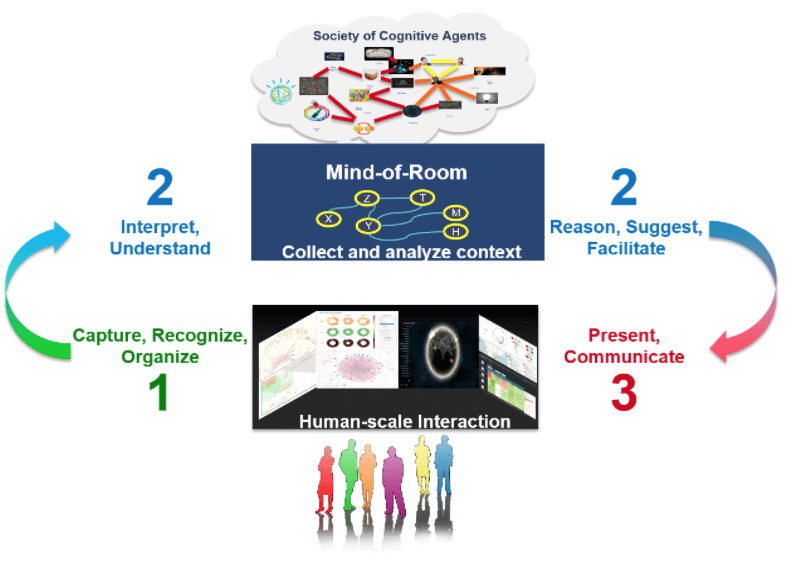
\includegraphics[width=0.5\columnwidth]{chapters/01_introduction/figures/cisl-cycle-graphic.png}
\caption{The flow of information through the elements of a cognitive and immersive system.}
\label{fig:cycle-cais}
\end{figure}
%%%%%%%%%%%%%%%%%%%%%%%%%%%%%%%%%%%%%%%%%%%%%%%%%%%%%%%%%%%%%%%%%%%%%%

We first introduce the notion of a \emph{cognitive and immersive
  system} (CAIS), which comprises three elements linked in a cyclical
flow as shown in Figure \ref{fig:cycle-cais}.  The first element is
responsible for perception and sensing within the environment that
contains the human agents (such as a room). Percepts come courtesy of
a range of sensors, such as microphones and kinects. From these
percepts, we receive information such as what was said, where users
are in the room, etc. The second element, upon receiving that
information, is responsible for interpreting, understanding, and
executing on the basis of that data. In this process, the CAIS may
employ reasoners, planners, databases, etc.\ to drive its
execution. The third element displays both percepts and the results of
processing these percepts in rich, multi-modal ways, such as showing
content on displays or speaking to the users of the system. As part of
the operation of the CAIS, we expect that it has access both to local
modules, as well as is able to make use of external machines and
services that are well-suited to specific tasks or domains. Perhaps
most important to note here is that these external services may be
requested for and opened by users of the system, but that one
reasonably expects that a CAIS should be able to handle these things
in a meaningful and useful fashion.
%% MATT2:  Previous sentence quite hard to understand.  Pls rework.
An important part of our system is that there are overseeing AIs
(agents) operating at the system level that can use the rest of the
system to assist and aid the humans and other AIs that are operating
within.  Thus, the overarching architecture is neither fully
centralized nor fully distributed, but aims to combine the strengths
of both.

Stemming from this overseeing AI, being that it captures all that goes
on within a CAIS, we can look to realize a number of useful
capabilities and principles. Most important here is that these stem
from a rigorous formalization, not from an \textit{ad hoc}
process. From these formal requirements and formalized operations, we
explore how this then also enables our CAIS to possess deeper levels
of understanding of human agents within the room, operating at a
proper theory-of-mind level~\cite{premack_does_1978}, and makes
capable automated means of reasoning, planning, and plan recognition.
An example of this is shown in the following section, and further
explored in Chapter~\ref{chap:planning}, utilizing reasoning to
determine the knowledge and belief of agents, and plan recognition of
what agents are attempting to accomplish to provide meaningful
assistance.

This dissertation is divided into three major parts. The first part
consists of this chapter and deals with the high level goals we lay
out for cognitive-and-immersive systems. We present a motivating
example, and discuss at a high-level abstract view what an idealized
CAIS may be able to accomplish. The second part of the dissertation
concerns mplementation of a real-world CAIS, focusing on two novel
compoments that allow us to to achieve mechanisms being multi-modal
and multi-user without having the system then be constrained to one
specific type of use case or domain. This part is encapsulated in
Chapters 2, 3, and 4. For the third part, which makes up Chapters 5
and 6, we now provide a formalization for these sorts of systems,
stemming from the implmentation in part 2, and then look to see how we
can utilize this for tasks in reasoning, planning, and plan
recognition. Finally, we conclude the work with a summary of our
contributions and recognize promising avenues of future work that
exist.


% 3. Motivating Example
\subsection{Motivating Example}

In this section, we provide an overarching motivating example to help
illuminate the challenges we hope to solve within this work. To help further
ground the work, we present an example that could be commonplace within a joint
meeting space, and does not include a contrived setup.

Imagine that within a CAIS, there are three humans, Alvin, Betty, and Charlie,
who are all jointly working on a shared problem. Alvin and Betty are standing
next to each other, while Charlie stands apart. There is content on the screen
that relates to the problem. Betty looks at Alvin, then points at a particular
region of the screen. Alvin, seeing that Betty is looking at him, looks at her,
then follows to where she is pointing at the screen. Charlie is not looking at
either Alvin or Betty, nor at the region of screen that Betty is pointing at,
but instead at some other region of the screen. Betty gestures at the region of
the screen that she is pointing at, and the content changes in some way. Alvin,
who is following along the pointing and gesture, perceives both the gesture, and
the content change on the screen, while Charlie does not. Alvin then points to
the screen and makes a gesture, changing the content on the screen for a second
time. Betty perceives the pointing and gesture that Alvin does, while Charlie is
still oblivious to it. The time for this meeting concludes, and Betty might
reasonably ask "is everyone on the same page?". Neither Alvin or Betty are aware
that Charlie is not, while Charlie is unaware of the changed content. The
CAIS steps in, saying that no, Charlie is not on the same page, and that here
is a summary of the actions of Alvin and Betty for Charlie to catch him up,
covering the content that Alvin and Betty had both pointed at, as well as
the content that had changed on the screen.

From this example, we see that the CAIS must possess a number of sophisticated
pieces of machinery. For the physical space, the CAIS must possess the capacity
of knowing who is using the system, the physical actions that they
undertake, and what these agents might say. The CAIS then must possess the
capacity to display information to the human participants and speak to the
human participants. Finally, the CAIS must be able to connect the physical
actions of the humans, to that of the content that is being shown within the
space, such that it connects Betty gesturing at the screen with content under
that gesture.


% 2. Requirements of a CAIS
\section{Requirements of CAIS}\label{ref:requirements_cais}

It should be noted that for a CAIS to be considered a truly
``intelligent'' room, it is not sufficient that the room be
intelligent about, for example, search queries over a domain $D$; the
room should also be intelligent about cognitive states of agents in
the room and their cognitive states towards $D$.

Despite there being a significant amount of work done in building
intelligent environments (of varying levels of intelligence;
\cite{coen_design_1998,brooks_intelligent_1997,chan_review_2008}),
there is no formalization of what constitutes an intelligent room and
what separates it from an intelligent agent.  Though
\cite{coen_design_1998} briefly differentiates an intelligent room
from ubiquitous computing based on the non-ubiquity of sensors in the
former, there is not any formal or rigorous discussion of what
separates an intelligent room from a mobile robot that roams around
the room with an array of sensors. As far as we are aware, this work
is novel in its act of providing a characterization of what separates
an intelligent room from an intelligent agent.

The requirements in question are cognitive in nature and exceed
intelligent rooms with sensors that can answer queries over simple
extensional data (e.g.\ a room that can answer financial queries such
as \textit{``Show me the number of companies with revenue over X?''}).
At a high-level, we require two conditions below hold:

\begin{itemize}
    \item $\mathcal{C}$ \emph{Cognitive}: A CAIS should be able to
      help agents with cognitive tasks and goals.  For instance, a
      system that simply aids in querying a domain $D$ is not
      cognitive in nature; a system that knowingly aids an agent in convincing
      another agent that some state-of-affairs holds in $D$ is
      considered cognitive. (Please see the appendix for more
      discussion of our usage of the term ``cognitive.'')
    \item $\mathcal{I}$ \emph{Immersive}: There should be some
      attribute or property of a CAIS that is non-localized and
      distinguished from agents in the room.  Moreover, this property
      should be \textbf{common knowledge}.\footnote{For our purposes,
        common knowledge as defined in Chapter~\ref{chap:formalizing}
        is that all agents know this property, and know that all other
        agents know it.}  (Note: this is not easily achievable with a
      physical robot, and this condition differentiates a CAIS from a
      cognitive agent.)
\end{itemize}

While we believe that $\mathcal{C}$ is fully realizable and is
achieved as part of this dissertation, $\mathcal{I}$ is certainly far
more ambitious, given the high level of sophistication necessary for
an implementation that satisfies this condition. As such, we posit
that for a true formalization to hold any water, it must stem from the
implementation and not vice versa. In this way, we can ground our
formalization in a working system that can properly showcase both the
formalization and our technology.

\begin{comment}
\footnote{This condition may not strictly be realizable,
        but the goal is to at a minimum build systems that approach
        this ideal condition.}
\end{comment}


% 1. Overarching Goals


% 4. Colocated vs Distributed

\section{On Co-location vs Distributed Usage}

Before continuing, we would like to take a moment to discuss the
beliefs of co-location vs distributed usage of these sorts of
technologies. Within this work, we present, and focus on, a vision of
how such systems can be applied and help with co-located
participants. While we do believe that elements of this work can be
applied to a digital domain, doing so fundamentally changes the
paradigm of collaboration. When working together, we use the humans
%% MATT2:  "use the humans"?  Not sure what is meant here.  Pls
%% clarify, refine.  Thx.
utilize different levels of coupling, increasing or decreasing based
on the extent of communication that is required by the task at
hand~\cite{salvador_denver_1996,olson_distance_2000}. However, it is
important that coupling is not a static concept through a task, rather
that it is dynamic, changing through the lifetime of a
task~\cite{jakobsen_up_2014}.  Within this coupling, we see rise to a
concept of ``we-awareness" amongst
participants~\cite{greenberg_implications_2016}, as they utilize some
level of implicit understanding of verbal and non-verbal
communications. These concepts do not easily transfer to distributed
digital systems wherein participants are no longer standing next to
each other, rather sharing a ``space'' through interfaces like video
chat. Take for example pointing to something on a screen. With two
people standing next to each other, and one pointing at a shared
screen, we can make reasonable assumptions regarding the cognitive
states of agents, what they're perceiving, and also regarding what
they might believe about each other and what each other perceives.

Moving to the digital realm, these concepts cannot be immediately
recast as is, as one must first design the necessary mechanisms to
capture that information, transmit it to the other participants, and
to do so in such a way that the many rich and subtle parts of that
face-to-face interaction are not lost. Given the complexity of that
task, and the research area unto itself it would require, we do not
attempt to give the parallels here; we instead focus just on the topic
of handling the work in the co-located version only.


% 5. Contributions of the Dissertation


% 2. Technology of a Cognitive and Immersive System
\chapter{Technology for Cognitive and Immersive System}

% 1. Introduction
\section{Introduction}

In the previous chapter, we introduced the concept of cognitive and immersive
systems, and we laid out high-level ideals. As stated there, before we may turn
to the act of formalization, we first turn our attention to the creation of
the CAIS architecture, along with a real-world implementation. As stated before,
this implementation will help inform and establish the possibilities of our
formalization process. This process stems that building a CAIS brings to bear
many fields of research, such as computer vision, natural language processing,
reasoning, planning, operating in harmony. Recent advances in each allow us
to create something that can be used for a range of use cases and possibilities.
Su~\cite{su_cognitive_2017} articulated a vision of some of the complex use
cases in which these systems can be brought to tackle including language
learning, assisting in decision making, and data exploration. While we target
decision making here, the usages of this technology are as such more far reaching.

In this vein, we view that the CAIS must be targeted and utilize technologies
that can be applied across domains easily and quickly. Additionally, we readily
demand that the system be multi-user and multi-modal to achieve the level of
immersion required by our earlier principles. We find it important to note here
that we look to achieve our multi-modality such that each modality is available
to all users at all times. Finally, we aim that our CAIS should be easy to deploy
and utilize across domains. In this fashion, we aim to support a number of
environments that can contain differing capabilities and configurations. For
example, within the work for this dissertation, we deploy the CAIS to two
configurations, one a lab wall and the other a 360$^{\circ}$ screen, shown in
Figure~\ref{fig:cais_environments}. 

\begin{figure}
\centering
    \begin{subfigure}[b]{.47\linewidth}
        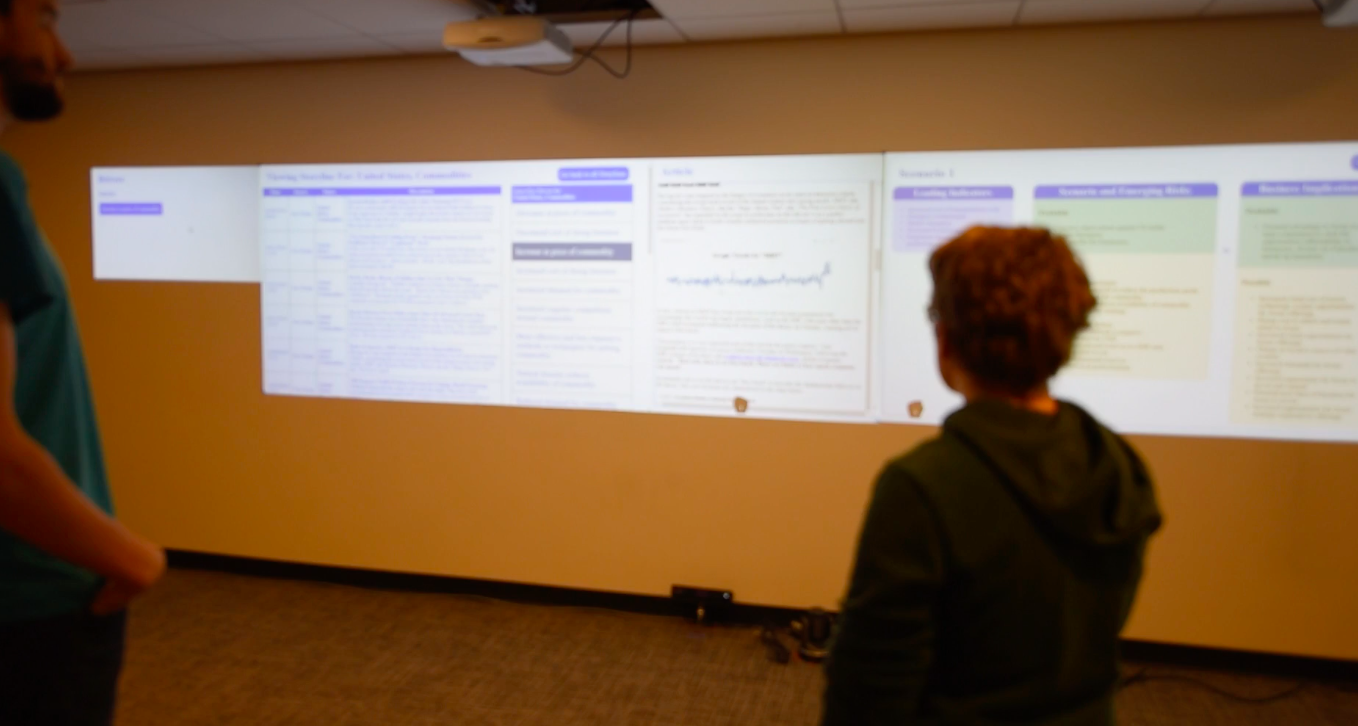
\includegraphics[width=\linewidth]{chapters/02_technology/figures/env_wall.png}
    \end{subfigure}
    \begin{subfigure}[b]{.48\linewidth}
        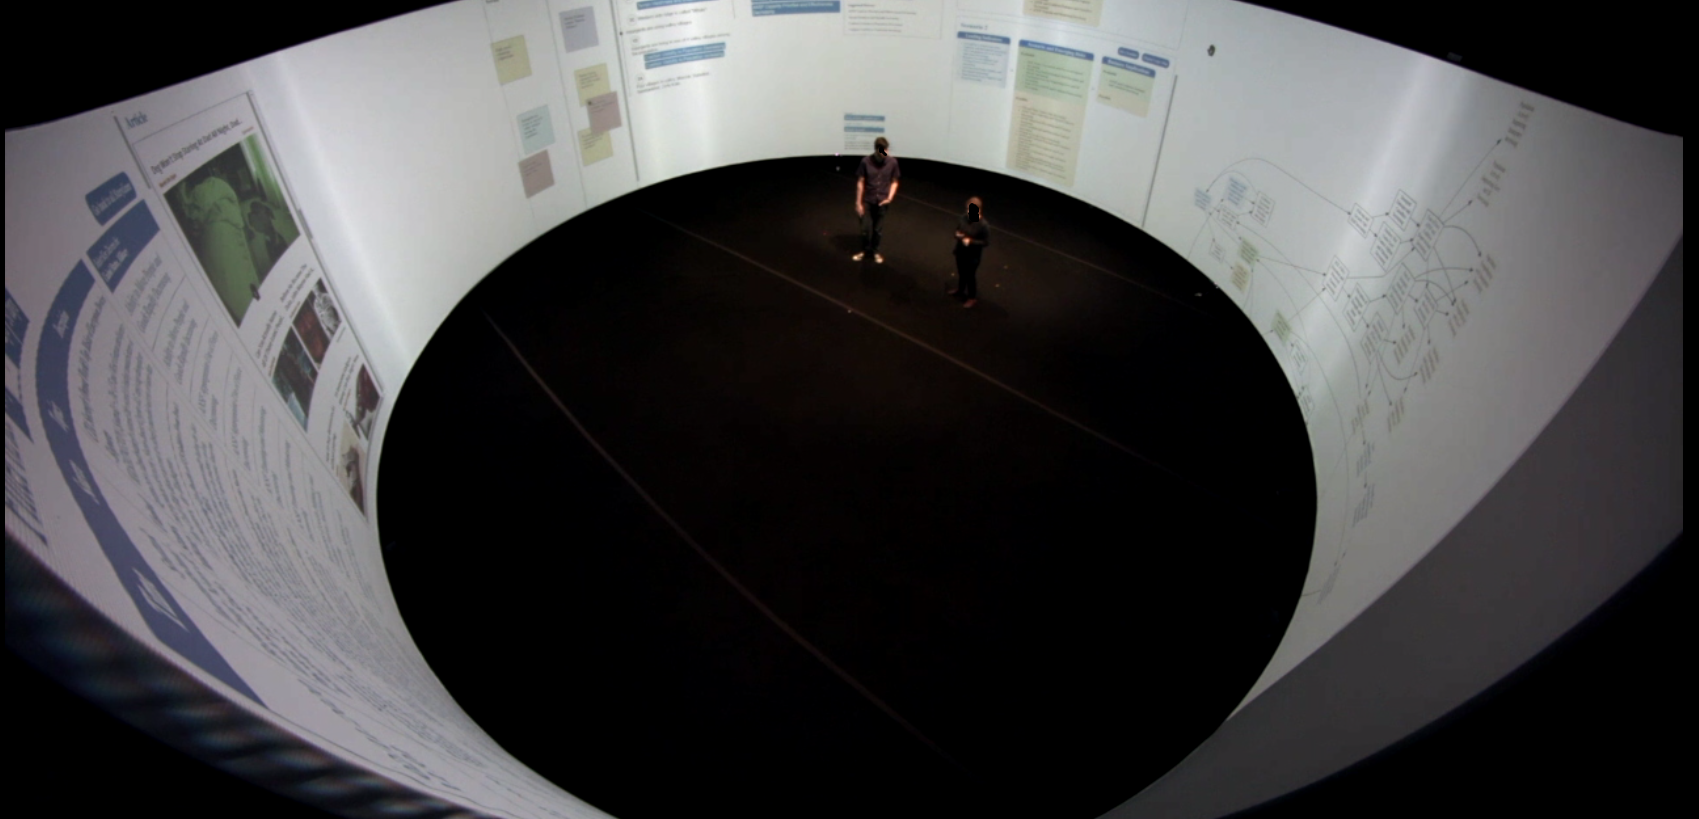
\includegraphics[width=\linewidth]{chapters/02_technology/figures/env_360.png}
    \end{subfigure}
    \caption{Two environments in which we deploy the CAIS, one a long flat wall and the other 360$^{\circ}$ screen.}
    \label{fig:cais_environments}
\end{figure}

% 2. Related Work
\section{Related Work}

There is a rich background of work for the design of multimodal systems, and more broadly the intelligent rooms
in which these systems are situated.

Historically, these systems have fallen into the category of ``smart rooms''
where multimodal input is much more of a necessity for more ``natural''
interaction than traditional desktop environments. In these multimodal
``smart rooms'', various efforts have been shown for picking up
where a user is pointing and using it in combination with
their voice to generate a command
\cite{bolt_put-that-there:_1980,carbini_wizard_2006,langner_multiple_2019,farrell_symbiotic_2016,kephart_embodied_2019}.
However, these systems hand-build their display layer and
content to embed the necessary instrumentation for combining speech
and gesture. Alternatively, \cite{coen_design_1998,brooks_intelligent_1997} demonstrate a system that
hooks into the X display server and could act on the content that was passed through
it from various applications, such as Netscape. While a very powerful approach, it
does not easily work across platforms, and that the security model of modern
applications such as Chrome renders the approach
increasingly impossible. Perhaps the most radical, \cite{roman_middleware_2002} propose an entire middleware infrastructure, similar to an OS,
to underpin these multimodal applications, but this approach
even more readily runs into the aforementioned bottleneck
in that all applications must be built from the ground up to
utilize this middleware, rendering it hard to reuse existing
content and displays.


% 3. Design Goals

% 4. Architecture
\section{Architecture of CAIS}\label{sec:cais_architecture}

In this section, we provide an overview of the general architecture that a
CAIS should follow for its implementation. From our experience, we believe
that the ideal architecture is one that is principally event-driven and
modular. By modular, we mean that each component of the system
should be implemented as a separate piece, following the UNIX philosophy for composable programs of 
``doing one thing and doing it well''~\cite{mcilroy_unix_1978}. The advantage of
this approach is that it allows one to easily substitute out pieces that with
something else, or not include them at all where it makes sense.
Figure~\ref{fig:cais_high_level} shows this concept for the input and output
layers of the CAIS. As shown, we show each piece of input hardware flowing
into its own worker module. The worker module is then tasked with turning the
raw input into something meaningful before it is passed along to be fused
with the other input mechanisms. In this way, the CAIS is responsible for
dealing with the fusion of sensors and that it is flexible in that not
all paths may be utilized.

\begin{figure}
    \centering
    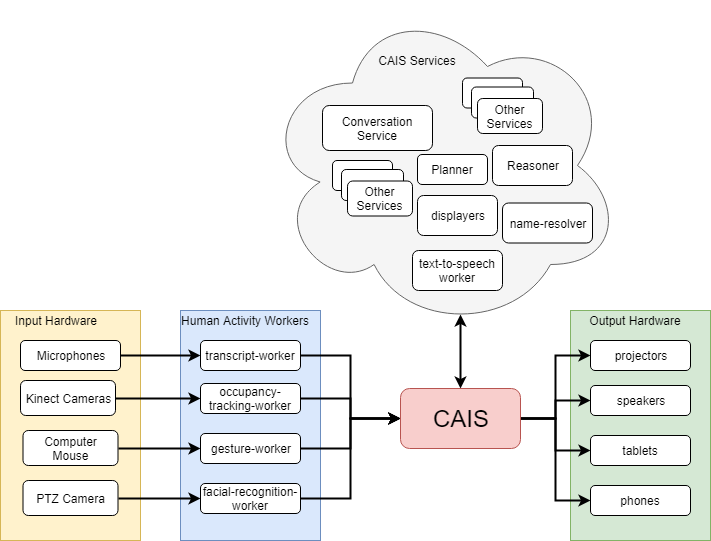
\includegraphics[width=0.5\columnwidth]{chapters/02_technology/figures/cais_high_level.png}
    \caption{High level diagram of CAIS architecture.}
    \label{fig:cais_high_level}
\end{figure}

As stated above, the architecture here is event-driven, such that workers can
be activated at any time, and then feeds through the CAIS, triggering further
modules as the event is fed forward. For example, the transcript-worker is
activated with the event of someone talking into the system. Important to
this model is the communication methods which we utilize within our system.
Principally, we utilize a distributed message queue wherein modules can
register as producers and consumers, allowing messages to be passed, which
act as the events of the system. One of the requirements here is that we
expect that multiple modules may consume from the same producer, allowing
a singular event to trigger multiple pieces downstream. Generally, each
``core'' module of the CAIS acts as both a producer and consumer, with
the exception of the edge modules, such that input modules (e.g. 
transcript-worker) are producers and the output modules (e.g. speaker-worker)
are consumers. For our purposes here, we utilize 
RabbitMQ~\cite{pivotal_software_rabbitmq_2020}, a commercially available
message broker that fits our needs. To accomplish the above message queue
requirement With RabbitMQ, we utilize a broadcast model where modules
subscribe to event topics, where each topic is made up of a number of pieces. 
Each topic is
unique to a given event, and that the topic pieces are specified in a manner of
least specific (e.g. the module name) to most specific (e.g. the event action).
Any number of consumers can subscribe to a given topic, each receiving the same
event. For example, the transcript-worker produces output on the topic
``transcript.result.interim'' (for in-progress speech transcription) and
``transcript.result.final'' (for finished speech transcription). Any number of
consumers could then listen to either of those channels, and be activated by
a transcription event. In rare cases, certain modules utilize RPC communication,
principally for modules that are hooked to a specific hardware device (e.g.
speaker-worker which is connected to a system's speakers). However, it's
expected that while communication to the module itself is done via a single RPC
queue, the module then broadcasts out events relating to what it is doing. For
the speaker-worker, this means that it will receive a sentence to output
via the speakers, and it will issue an event ``speaker.speak.begin'' before
it starts playing the sound, and ``speaker.speak.end'' when it finishes, which
any module can subscribe to.

Finally, for services that are not necessarily core to the CAIS itself, but
rather contain information or outside capabilities, we largely rely upon
utilizing standard TCP calls to these services. These services are, but not
limited to, things like databases, prover, external APIs.

A limitation of this approach is that each new link between modules introduces
additional latency to the system. However, within everything running on a high
speed connection, the added latency is roughly ~8ms per link. This throughout
is not largely felt by the user over the bottleneck of slower operations
involved with calling some of the external services and complex operations
of the CAIS, such as transcription service for parsing microphone input.

We are confident in our approach, and are in good company with  prior work that
followed a similar approach, such as the work done by
Brooks~\cite{brooks_intelligent_1997}. However, unlike this prior work, through
the use of RabbitMQ, the links between modules are that of topics, and not
necessarily hard coded agent links.


% 5. Modules
\section{Implemented CAIS Modules}

\input{chapters/02_technology/05_modules/01_intro.tex}

%  1. transcript-worker
\input{chapters/02_technology/05_modules/05_transcript-worker.tex}

%  2. conversation-worker
%  3. MUIFOLD
%  4. spatial-context-worker
%  5. Reagent
%  6. orchestrator
%  7. executor
%  8. display-worker
%  9. speaker-worker



\chapter{Reagent: Enabling Interaction with Arbitrary Web Content}\label{chap:reagent}
\blfootnote{Portions of
  this chapter previously appeared as:
  \begin{enumerate}
    \item M. Peveler, J. O. Kephart, and H. Su.  Reagent: Converting Ordinary Webpages into Interactive Software Agents.  In \textit{Proceedings of the Twenty-Eighth International Joint Conference on Artificial Intelligence}, pages 6560–6562, Macao, China, Aug. 2019
    \item M. Peveler, J. O. Kepahrt, X. Mou, G. Clement, and H. Su.  A Virtual Mouse Interface for Supporting Multi-User Interactions.  In \textit{Proceedings of the 22nd International Conference on Human-Computer Interaction}, Copenhagen, Denmark, July 2020. Springer
\end{enumerate}}
 
\section{Introduction}

With the growing ubiquity of voice-activated assistants like Siri and Alexa, society is
quickly acclimating to interacting with AI as we do with our fellow humans. Now under development is
a new generation of more sophisticated assistants centered around 
cognitive spaces that are designed to help scientists, business users, and students with
cognitive tasks such as data exploration and analysis~\cite{kephart2018cognitive}, decision making~\cite{farrell2016symbiotic}, and learning languages~\cite{allen_rensselaer_2019}.

Practically all of these cognitive applications entail some sort of interaction with data that
is based on multi-modal inputs that include speech, pointing and gesture. To date, the assistants have 
supported such interactions by reading data from a database and displaying it in the form of tables or 
plots through web pages that are specially instrumented to capture pointing events. A stream of utterances 
is converted into a text stream by a speech-to-text engine and combined with the stream of pointing events 
to derive user intent, i.e. a parameterized command that is then executed by orchestrating one or more services 
and rendering the output on a display and optionally as synthesized speech played through a speaker. A 
major bottleneck in the creation of such cognitive assistants is that creating specially-instrumented web 
pages is labor-intensive. Unless this bottleneck can be removed, it seems unlikely that multi-modal cognitive
assistants will become anywhere near as pervasive as the present generation of less-sophisticated bots.

In this paper, we describe \textit{Reagent}, a novel technology that reduces the above-mentioned bottleneck by
readily converting ordinary non-instrumented webpages containing structured data into
software agents with which one can interact naturally, via a combination of speech and
pointing. \textit{Reagent} combines streams of semantically-meaningful mouse events with
speech transcriptions to derive and execute parameterized commands that represent user
requests to visualize, extract, query, sort, filter, analyze, or otherwise manipulate data
displayed on webpages. Command execution entails displaying the requested information in the
original webpage or in a dynamically-constructed one, as well as playing synthesized speech.
\textit{Reagent} automatically infers mappings from event labels to human-friendly terminology,
or when necessary learns them actively from the user. 

\textit{Reagent} takes advantage of the fact that web pages are highly structured, plus
emerging website accessibility conventions and standards that embed
information that helps interpret elements that are displayed on a given web page. 
For example, there exists a large body of guides on accessibility for sites which include the W3C Standard
Web Content Accessibility  
Guidelines\footnote{https://www.w3.org/WAI/standards-guidelines/wcag/} or a
Voluntary Product Accessibility 
Template\footnote{https://www.section508.gov/sell/vpat}. This accessibility
is aimed at improving the experience of people with disabilities, and who might
not be able to fully see and visualize the content of page. These users rely
on things like screen readers which traverse the semantic elements of a page
and speak the contents to the user. To accomplish this, these elements utilize
hidden, non-visible attributes that help to establish semantic understanding of
content on the page (e.g. headers and links) as well as showing information on
hovering on certain elements (e.g. column headers and images). Taking column headers as an example, 
while they may often be abbreviated when displayed to the end user, the full text is often available
when the user hovers over the abbreviation, i.e. the information is embedded in the page as a hidden attribute.

The remainder of the paper is organized as follows. After discussing related prior research, we describe
Reagent and its relationship to a larger immersive systems architecture in which it is embedded. We then describe a use case illustrating
how Reagent can be used to collaboratively build an ontology from scratch, pulling information from pages as users navigate and interact with them. We then perform an experiment to assess how broadly
applicable Reagent is to web pages encountered in ordinary use, finding that it works for approximately 80\% of nearly 200 popular web pages that we surveyed.
We conclude with a summary and some thoughts about future directions for this research.

\section{Prior Work}

Work on Reagent principally concerns bringing together two discrete lines
of work. The first is prior work on building intelligent system that are
capable of combining multimodal input to generate an intent for the user,
which was covered in Section~\ref{sec:cais_prior_work}. On second
line of interest, we look at the rich research on automatic extraction of
information from webpages and the lessons learned there, especially in how
they might work with ontology building. Cimiano et
al.~\cite{cimiano_towards_2004} and Storey et 
al.~\cite{storey_ontology_2005} propose frameworks on parsing
important information from web pages, which would be then encoded into RDF
structures. Gangemi~\cite{gangemi_comparison_2013} provides a recent
overview of available technologies in this space.
However, these approaches generally focus on the use of just natural
language understanding over the entire page for key terms and relations,
and not necessarily leveraging the increasingly rich ways the data may
be shown in a page that require true DOM traversal and analysis. However,
in analysis and automatic parsing of the DOM structure, we are informed
by prior work on taking into account elements that are ``noise'' (e.g.
ads and popups) which might look well-structured, but that the user most
likely does not care about. Gupta et al.~\cite{gupta_dom-based_2003}
utilizes the full DOM-tree to determine relevance of elements.
Joshi and Liu~\cite{joshi_web_2009} utilize both DOM traversal and NLP
to determine salient details. Sun et al.~\cite{sun_dom_2011} utilize a
algorithm that considers content density within nodes. Our current work
focuses on automatic analysis of elements that rarely, if ever, appear
within this ``noisy'' data, but is important to consider as we expand
Reagent to further domains. Finally, in the realm of understanding purely
tabular data, Hackinger~\cite{hackinger_datagorri:_2018} proposes a
system similar in some regards to \textit{Reagent}, but that it requires
for any new site the human to first identify the table on the page and
to present a ``template'' on how it should be parsed, acting far less
autonomously than \textit{Reagent}. These works inform our approach
on building \textit{Reagent}, but it is important to note that our
end-goal, principally in automatic on-the-fly webpage parsing and
ontology building for use in multimodal applications, is different.

\begin{comment}
% this is a slimmed diagram of the one shown in chap 2, so ignored
\begin{figure}
    \centering
    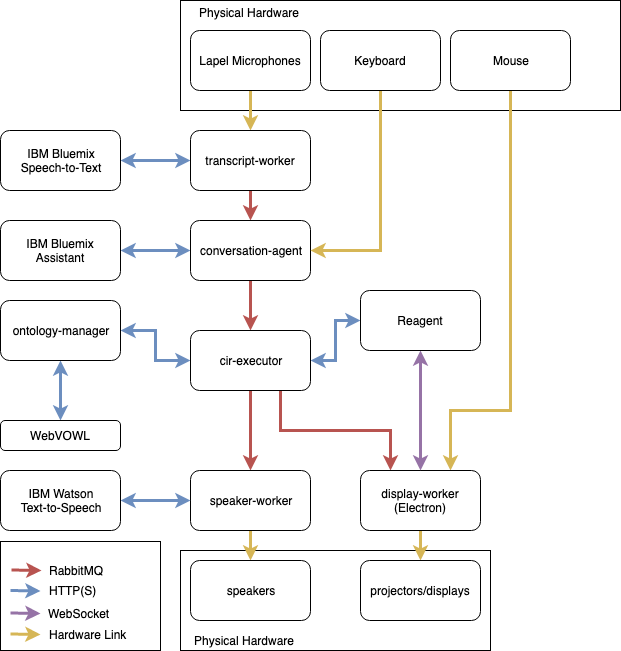
\includegraphics[width=0.45\textwidth]{chapters/03_reagent/figures/cir_diagram}
    \caption{Diagram of the Cognitive and Immersive System for Reagent}
    \label{fig:cais}
\end{figure}
\end{comment}

\section{Reagent}\label{sec:reagent}

The \textit{Reagent} system allows us a way to hook into the content that is
shown within the Electron framework discussed in Section~\ref{sec:display-worker}. The
system is broken up into two components, a central server and then the clients.
The central server is used to handle communication from the clients and the
larger CAIS architecture, as well as store information coming from the clients
for reference. This information includes the type of semantic elements exist on
the page, as well as an event stack for recorded user interactions within any
webview. Communication between the server and the clients is handled by using
websockets which facilitates real-time communication of data. To handle requests
from the CAIS, the server implements a RESTful API. The client are inserted as a
transparent layer on top of any opened webview within the system.  This
transparent layer then sets up a connection back to the central server, and then
semantically parses the page using standard DOM traversal via JavaScript
to identify key HTML structures with which a user
might interact with (e.g. a table or a plot), and uses this information to bind
appropriate event handlers to listen for user interactions, as well as for any
changes to the page's content. More specifically,

\begin{enumerate}
    \item Electron pre-loads the \textit{Reagent} system on top of the webview, and injects a websocket connection allowing it to communicate with the open webview and receive JSON-formatted events into an event buffer.
    \item Electron emits a ``DOM Ready'' event to signal that the page has finished loading, whereupon \textit{Reagent} scans the page to see if it can detect any major HTML elements it should parse and bind to (e.g. a table).
    \item \textit{Reagent} injects additional code specific to the detected HTML elements that binds event listeners to these elements as well as assigning each a UUID --- an approach that makes \textit{Reagent} readily extensible to new types of elements. (We have implemented domain-independent layers designed for general tables and for plot.ly plots, and allow for domain specific layers as well.)
    \item Next, \textit{Reagent} creates a MutationObserver\footnote{https://mzl.la/1exU78d} to watch for any changes to the page. If changes are detected, it performs any necessary re-injections and re-bindings to ensure that all relevant elements remain instrumented.
    \item Finally, \textit{Reagent} sets up a listener such that if the webview
    is closed, the client disconnects and the server is alerted.
\end{enumerate}

This sequence of events is illustrated within Figure~\ref{fig:reagent}. As an example, we discuss how the
Reagent system would bind to a HTML table and the sorts of queries it would allow for from the user. A perfect data table
is made up of some number of columns and rows where the first row, if marked with the ``th'' tag, should be viewed
as a header row with labels for the columns, and then all subsequent rows marked with the ``td``` tag as data. Reagent
scans the table, generating a list of the column names and some simple heuristics about the structure of the table. Next,
assuming that Reagent has never seen a table on this site before, it first takes all of the headers and attempts to
normalize them as appropriate for its datatype using NLTK and WordNet. Take for example, a column labelled ``won''
for a column with numeric information. Here, the system first casts the word to the present tense of the verb (``win''),
and then pluralizes on its noun form (``wins''), giving us a title more likely to be said by humans. From here, we then
use WordNet to find the variations of the word (on both its noun and verb forms) and add them as entities, if missing,
to Watson Assistant to be used for intent classification on future queries.
Finally, the system binds listeners for user interaction, which in the case of a simple table would be if a user clicks on
a cell in a table or leaves their mouse hovering over it for greater than a second. For any interaction, the client
communicates with the server, which saves a JSON object of the interaction which contains what webview it occurred in,
generated reagent UUID of the element, what row/column the cell was in, contents of the cell, and the type of interaction
it was (e.g. mouseover or click).

During the scan of HTML elements, the system is capable of taking advantage of
content added for accessibility reasons. For example, in
Fig.~\ref{fig:reagent_use_case_2}, the column for ``appearances'' was labelled ``APP''.
\textit{Reagent} identifies tags that may indicate more human-friendly terms,
such as tooltips that reveal explanatory text when a user hovers over an
element, and uses approximate text matching to infer likely associations where
possible.
In cases where the system is unable to disambiguate the semantic information, it
solicits a definition from the user. For example, with the ESPN table, the
system would ask the user (via synthesized voice) to mouse over ``the column
labeled  \textit{A}'' and state what is the attribute. Upon hearing ``Assign
attribute \textit{assists} to this column'', \textit{Reagent} stores the
mapping in a dictionary, whereupon it becomes available to any subsequently
accessed bound elements on the same webpage or host site.

\begin{figure}
\centering
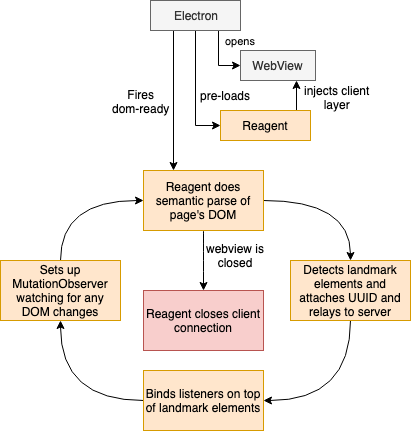
\includegraphics[width=0.45\textwidth]{chapters/03_reagent/figures/reagent.png}
\caption{Flowchart of the Reagent System.}
\label{fig:reagent}
\end{figure}

Through the transparent layer and central server described above, \textit{Reagent} enables
the executor to handle a wider range of queries that pertain to references
to the content within open webviews. At its most basic layer, the user can
query the system for the contents of the full table, what are the columns in a
table, as well as asking queries about statistics (e.g. max, min, or average)
of any given column. By capturing the interactions, it then allows the system
to handle queries that are for relative locations within the interacted with
element. For example, Figure~\ref{fig:reagent_use_case_2} illustrates the state of the
display after the user has opened an ESPN football team roster webpage and
asked the system ``Show in a new table rows where \textit{appearances} are
greater than 35.''. Equivalently, the user might have asked ``Show in a new
table rows with this column greater than this.'' while pointing to a cell
under the column `APP' with the value of 35.\footnote{For a fuller set of
capabilities that includes query, sorting, and simple analytics like averaging,
a link to a demo video is available at
\url{https://www.youtube.com/watch?v=qVmY3YmNzGE}}.


\section{Virtual Mouse Interface}

Given Reagent, we now describe how we utilize it on building
a \textit{Virtual Mouse Interface} into the opened pages.
Leveraging input from a pointing device (e.g. Kinect camera or
MUIFOLD) and Reagent systems, this interface allows users to
interact with content as well as to guide multi-modal interactions.
This interface gives each user the equivalent of their own
personal mouse. The virtual mouse, under the hood is not one
dedicated component, but rather conglomeration of functionality
across modules described above. To start, from our pointing device,
we expect that it provides us with an absolute [x,y] coordinate for
the screen at which a user is gesturing, with a unique ID per user.
This is sent into the display-worker, which then displays an icon to
the user on the screen that represents where they are pointing at that
time, as well as the mouse action they are doing. This icon updates at a
constant rate for the user, and scales to many concurrent users, where
there is (due to RabbitMQ) a delay of about 4-8ms, which is largely
imperceptible to users. In addition to the display-worker, our pointer
system sends the pointing and action data to the orchestrator. The
orchestrator communicates with the display-worker to translate the
absolute [x,y] coordinate into a relative [x,y] coordinate within a
specific webview. From here, it communicates with Reagent in a number of
ways. For each payload that it sends along, and the subsequent action
JavaScript event that Reagent generates against a given WebView, the
unique user ID is passed, which Reagent binds to the generated events
that are dispatched to the page. First, it is important to denote that
the orchestrator sets a a limiter on the number of actions that can
flow through the system, which is roughly 75ms per action type, which
allows adequate throughput for the system for a number of users such
that they do not notice lag while also not sending too much information
to the page and potentially causing a slow-down. Below, we describe 
the two types of actions with which we concern ourselves with, mouse
and scroll.

\subsection{Mouse Actions}
Mouse actions represent the principle way in which people interact with the
page. This includes the use of the left and right mouse buttons, though we
mainly focus on the usage of the left button here. The mouse button itself can
be thought of as being in three potential states, being held down for any period
of time (MouseDown), being released after being held down for any period of time
(MouseUp) and a rapid push down and release of the button (Click). Additionally,
there is the act of just moving the mouse itself (MouseMove). To start with
these actions, the orchestrator first sends a MouseMove event to Reagent, which
then gets dispatched against the webview. From this, Reagent returns the element
that the mouse is currently over. The orchestrator stores this element and if it
different from the last stored element, issues to Reagent a leave event
(MouseOut) on the old element and an enter (MouseEnter) on the new element. This
chain of events allows for triggering of hover type events on a site for the
given elements affected as you move your cursor across a page. Finally, it takes
the mouse action (MouseUp or MouseDown and possibly Click), and sends that to
Reagent to issue against the page. In all of three of these cases,
Reagent sends details about the element that was clicked on, such that the
orchestrator can drive subsequent interactions on it, such as if clicking on a
form input, can ask the user what value do they want to input, which is picked
up via voice input.

\subsection{Scroll Actions}
For scroll actions, a more involved sequence is followed to determine what type
of scroll is meant by the user. Webpages may implement scroll to mean just
moving around the content that has overflowed from the available displayed space
(such as scrolling down on a news article), which is referred to as a
ScrollEvent. Alternatively, they may use scroll to control zooming in and out of
the content, or panning (common in graphs or maps), where these are WheelEvents.
However, for both, we require the difference between the current mouse position
and the previous mouse position to perform the action, which is stored within
the orchestrator. To determine the appropriate action (especially on a page that
includes both overflowed content and a graph), the orchestrator first sends a
WheelEvent to Reagent. Reagent returns the event that was acted upon, as well as
if the MutationObserver it attached to the page detected any changes to that
page. If there are no changes, than the system determines that the user's
intention was not to zoom or pan, but to simply scroll the page for overflowed
content, at which point a ScrollEvent is issued to Reagent, and the page content
is shifted.


\section{Sample Use Case}

To demonstrate the power of the \textit{Reagent} system, we demonstrate it within a 
toy domain of analyzing football teams within the premier league team and building 
an ontology in OWL~\cite{staab_web_2004} around it. The system starts with no knowledge within the ontology
and the goal is at the end to have built up a minimal relationship graph of the couple of 
entities we encounter as well as their properties, as automatically as possible.
To accomplish this, we utilize content from the websites ESPN and SkySports. The
output of the UI that is displayed to the user is shown in the following figures.
Within the figures, the top left contains the current site/table being
inspected. Underneath that, there is a display to show the current state of the ontology as it 
is being built, shown using WebVOWL~\cite{lambrix_webvowl:_2015}. On the right is the
running transcript of the system with queries from the user being prefixed with a yellow 
``Person'' and the system's responses being prefixed with a blue ``Watson''. 

%\begin{figure}
%\centering
%\includegraphics[width=0.45\textwidth]{figures/skysports_premier.png}
%\caption{Premier League Table from SkySports.}
%\label{fig:skysports_premier}
%\end{figure}

\begin{figure*}[hbtp]
\centering
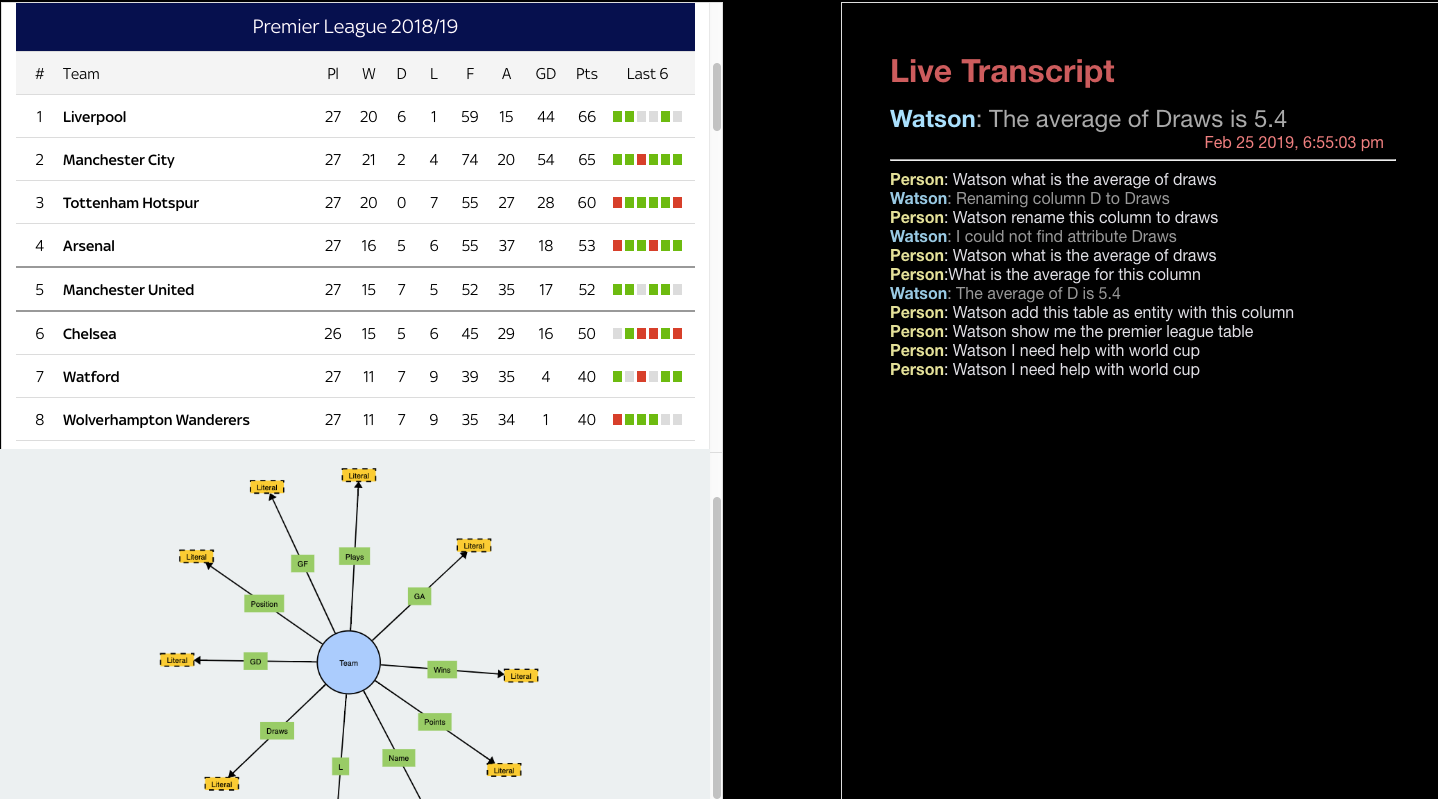
\includegraphics[width=0.8\textwidth]{chapters/03_reagent/figures/use_case_1.png}
\caption{Display of system after adding Team entity.}
\label{fig:reagent_use_case_1}
\end{figure*}

To start with, we open a page from SkySports that shows the current standings
of all teams in the football premier league~\cite{skysports_table}. To begin building
our ontology, the user can point at the displayed table and then state ``Add this table
as entity {\em team}'' or alternatively point at the column marked ``Team'' and say ``Add this
table as entity using this column''. The executor will contact \textit{Reagent} to get the columns
of the table under question. From there, the executor will send the list of columns, as well
as the entity name to our ontology as a simple JSON object, which in then converted by an
ontology pipeline into the appropriate OWL RDF structure to be stored, marking the entity as a 
Class and the columns as Object Properties linked to the class, and pointing at concrete 
Literals. After this step is completed, all entries in the table are then saved as instances
for that Class, ready to be queried. Additionally, anytime a user comes back to this page,
or a page that has a table of nearly identical structure, the system will automatically infer that the table
is of the Team class, along with automatically transforming any abbreviated columns to known
attributes if possible. Either before or after adding an entity to the ontology, a user can always go and
fill in the gaps as necessary in the system's understanding of the columns. For example, in the case of 
SkySports, while the first 4 columns have a title tag (displayed when hovering over the abbreviation), 
the rest do not and so the system saves them only as abbreviations (e.g. ``D'', ``L'', etc.). 
Additionally, while we can query the system for values of the fully named attributes, we cannot at this
time get anything for the abbreviations for what they stand for. For example, if the user
tries to ask ``What is the average of draws'', the system will respond with 
``I could not find the attribute draws''. To remedy this, the user can point at one of these
columns and then issue a new name for the column. For example, to update the
label marked ``D'', the user would point at the column and say ``Rename this column
name to Draws'', which gets automatically mirrored to our
ontology. Following this, the user can then repeat a request for the
average of draws and the system will now successfully respond with ``The average of Draws is 5.4''. The result of this sequence is shown in Figure~\ref{fig:reagent_use_case_1}, wherein we still have several more attributes that
have to be renamed due to lacking the title tag, using a similar command as
above.

After being satisfied with the constructed ``Team'' entity, the user may want
to then look at the players of one of these teams. To
do this, we open a page of a team (e.g. Manchester United) from ESPN~\cite{espn_squad_table}. When we open
the page, the system scans the table, sees if the table matches
any saved entity, which is just ``Team'' at this time and as the columns does not match the ``Team'' entity's attributes,
the system states ``I do not recognize this entity. Please add it''. Similar
to the previous entity, the user
can save the table as a new entity by first pointing at it and then saying ``Add this table as entity 'player''', which
adds a new entity ``Player'' to our ontology along with all of the columns in the
table in the same process as before. A new Player entity then appears
alongside the Team entity in the Ontology Viewer of the display, which
is shown in Figure~\ref{fig:reagent_use_case_2}.

In this case, all of the terms have title tags and so are all properly labeled when they were added, so the user does not have to do any further renaming. The user can
now query the system about these saved attributes, such as pointing at the first
row in the table and asking ``How many appearances does the player have'' which
the system responds with ``The player has 24 appearances''.

\begin{figure*}[hbtp]
\centering
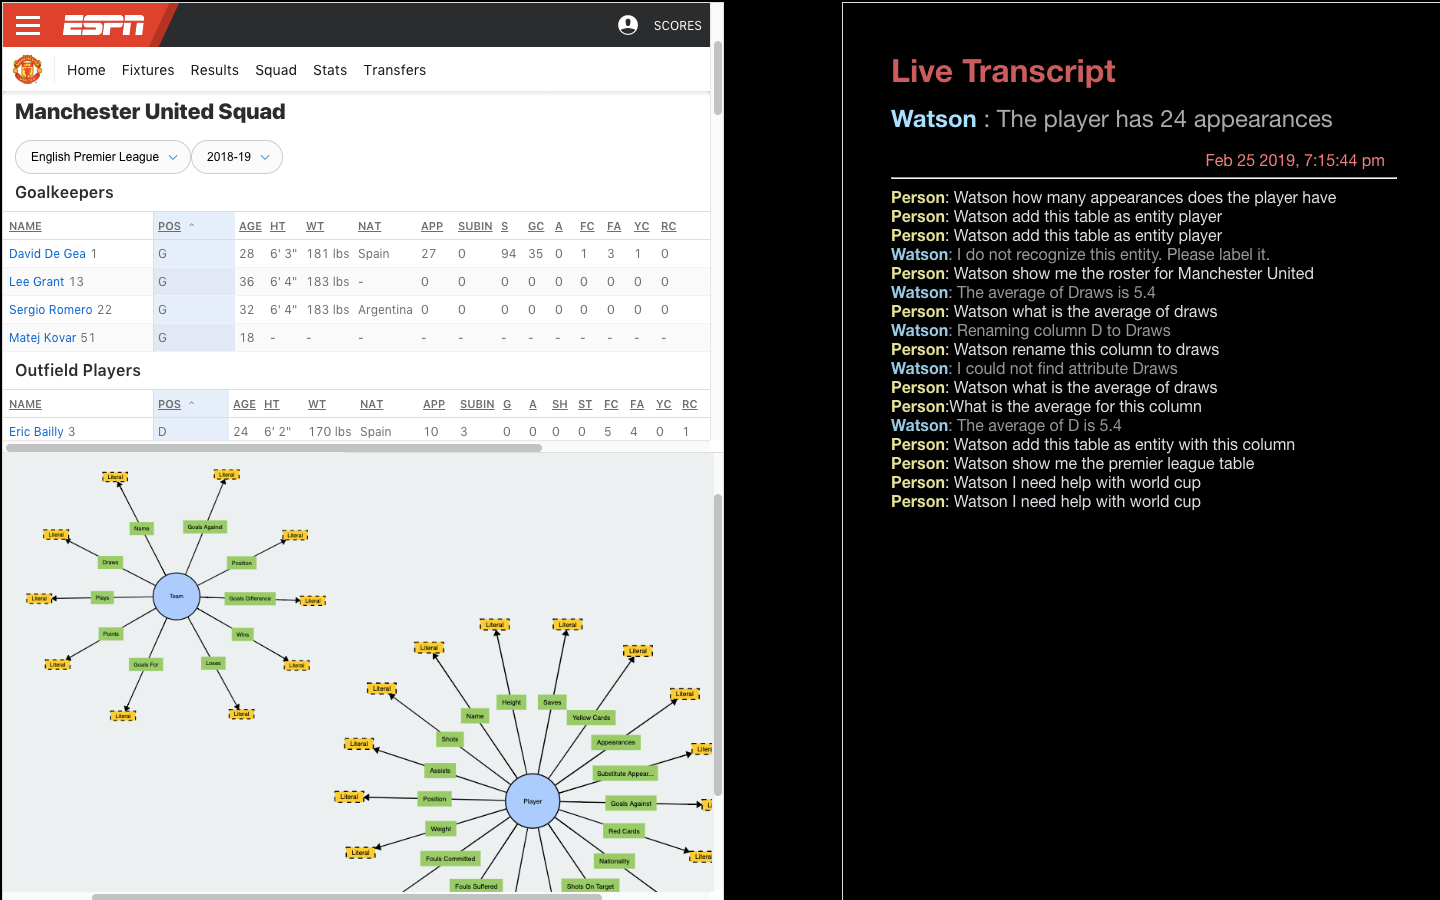
\includegraphics[width=0.8\textwidth]{chapters/03_reagent/figures/use_case_2.png}
\caption{Display of system after adding the Player entity}
\label{fig:reagent_use_case_2}
\end{figure*}

To complete our basic ontology, the user can now add a relationship
between the two saved entities. To do this, the user can simply issue
the query ``Add relationship part of between entity team and player''. The
system then adds a new Object Property link between the two marked as 
``partOf'', as shown in Figure~\ref{fig:reagent_use_case_3}. Through this connection,
the user can now start issuing queries that utilize information from both of the opened tables. For example,
the user can ask ``How many wins does the team of this player have?'' while pointing
at the player table. The system will look up who that player's team is, cross-reference it
back to the prior table, and extract the requested information, outputting it to the user.

\begin{figure*}[hbtp]
\centering
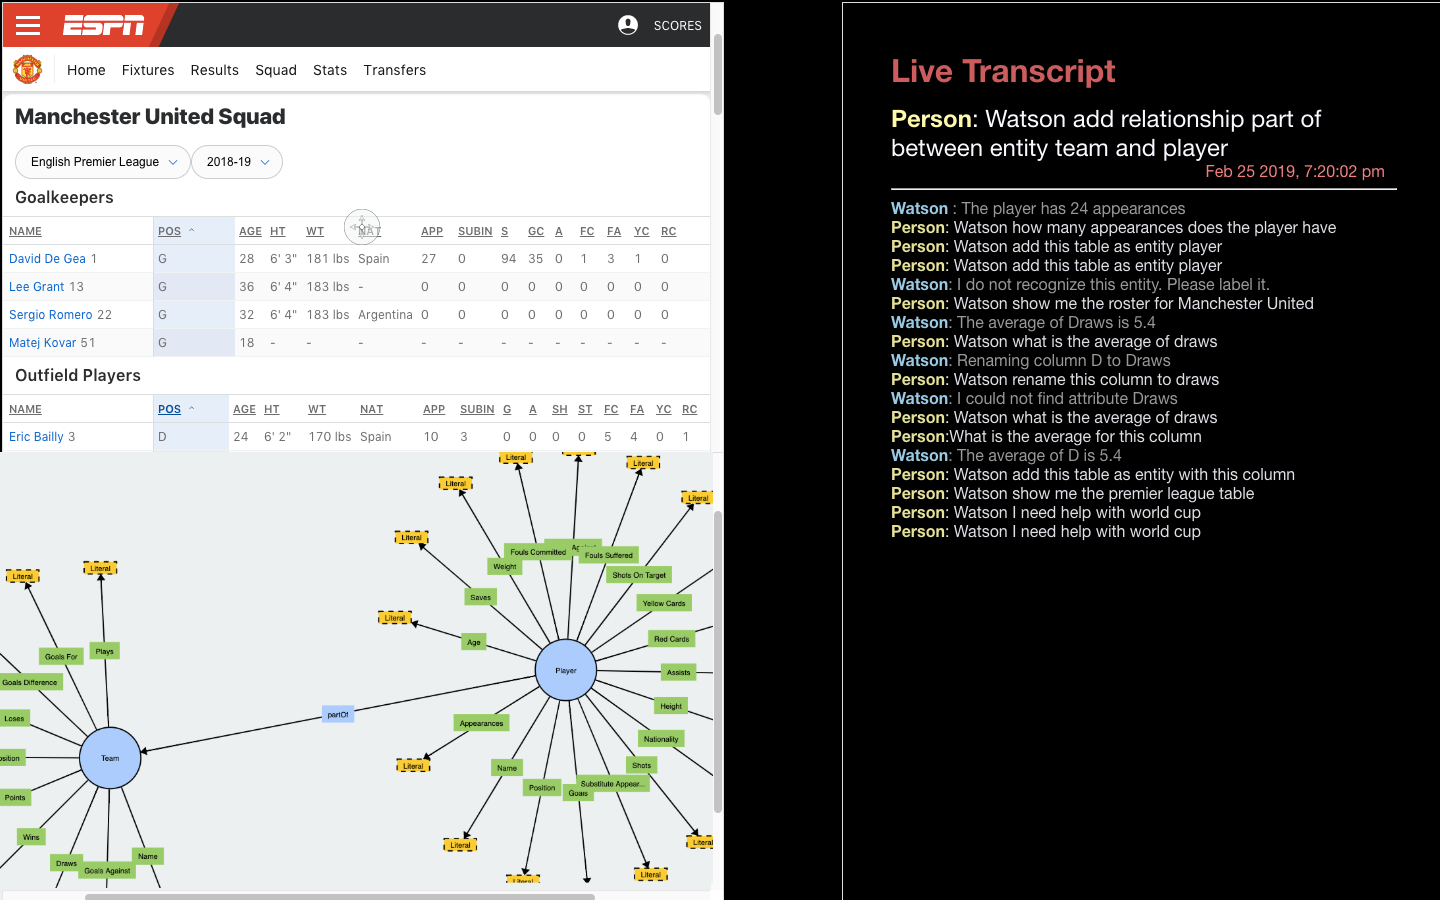
\includegraphics[width=0.8\textwidth]{chapters/03_reagent/figures/use_case_3.png}
\caption{Display of the system with the final ontology.}
\label{fig:reagent_use_case_3}
\end{figure*}

After building this ontology, whenever a user goes to a page that contains
similar content, the system will, as before, attempt to determine if the
content is of a known entity based on the table's columns, even if
the table has more or fewer attributes than have been seen. If a table is seen
with more attributes than saved in our ontology, it will ask the user if they
wish to add the attributes to the saved entity.


\section{Experiment}

To assess Reagent's ability to support natural interactions between users and third-party web pages that are typically encountered in the wild, we conducted an experiment involving nearly 200 web pages. We briefly describe the experimental setup and data collection, and then present the experimental results.

\subsection{Experimental Setup and Data Collection}
In order to obtain a collection of popular websites that contain data in tabular form, we used the Alexa service~\cite{noauthor_top_nodate}, which provides a list of the top sites viewed per month. From that service, we chose the top 10 sites in the ``Sports'' and ``Business'' categories, and filtered out those sites that contained only articles or pictures about the subject material. We crawled each of the remaining websites to generate a list of candidate pages that each contained at least one data table. In some cases, sites contained clusters of pages that were structurally identical but contained different content. For example, each team in the English Football League may have pages containing structurally identical tables, but of course the content is particular to each team. In this case, we randomly select a single representative from that cluster so as not to bias our statistics.

We then measure for each site the following quantities:
\begin{itemize}
    \item {\bf Pages.} Number of pages analyzed for the site.
    \item {\bf Tables.} Number of tables found among the pages analyzed for the site. Only the first table on each page is analyzed further.
    \item {\bf Failed.} Number of pages that Reagent was unable to parse within a timeout period of 15 seconds. For most pages, parsing takes 1-2 seconds, but for SPA type sites (where the body content dynamically loads after the rest of the page) it can take about another 2-4 seconds. Depending on how content (including ads) is loaded, a few pages take much longer because Reagent re-starts parsing whenever the page content changes.
    \item {\bf Columns.} Total number of columns among the tables analyzed for a site.
    \item {\bf Verbatim (V).} Among the columns analyzed for a site, the number for which the visible column headings are directly understandable.
    \item {\bf Interpretable (I).} Among the columns analyzed for a site, the number that, while not directly understandable, are interpretable through the use of tooltips or other metadata contained within the web page, possibly assisted by WordNet.
    \item {\bf Non-interpretable (NI).} Among the columns analyzed for a site, the number for which Reagent is unable to associate a human-understandable term, and which must therefore be defined by the user.
    \item {\bf Verbatim-Strict.} Among the tables analyzed for a site, the number for which {\em all} visible column headings are directly understandable.
    \item {\bf Interpretable-Strict.} Among the tables analyzed for a site, the number containing at least one {\bf interpretable} column.
    \item {\bf Non-interpretable-Strict.} Among the tables analyzed for a site, the number for which Reagent is unable to associate a human-understandable term for at least one column.
    \item {\bf Success Rate}. The percentage of column headers at a given site that can be interpreted correctly by Reagent, either verbatim or by using auxiliary information.
\end{itemize}

\begin{table*}[hbtp]
\centering
\begin{tabular}{ |c|c|c|c|c|c|c| }
 \hline
 Site & Pages & Failed & Cols & V & I & NI \\
 \hline
 ESPN & 93 & 19 & 1184 & 199 & 623 & 362 \\
% # of Pages: 93
% # of Pages Failed: 19
% # of Columns: 1184
% .  # abbreviated: 985
% .  # abbreviated, could expand: 623
% .  # not abbreviated: 199
% # of Tables: 196
% .  # of Tables with abbreviations: 132
% .  # of Tables with abbreviations with titles: 39
 \hline
 CricBuzz & 3 & 0 & 63 & 30 & 26 & 7\\
% # of Pages: 3
% # of Pages Failed: 0
% # of Columns: 63
% .  # abbreviated: 33
% .  # abbreviated, could expand: 26
% .  # not abbreviated: 30
% # of Tables: 5
% .  # of Tables with abbreviations: 4
% .  # of Tables with abbreviations with titles: 3
 \hline
 SkySports & 9 & 1 & 86 & 17 & 43 & 26 \\
% # of Pages: 9
% # of Pages Failed: 1
% # of Columns: 86
% .  # abbreviated: 69
% .  # abbreviated, could expand: 43
% .  # not abbreviated: 17
% # of Tables: 14
%    # of Tables with abbreviations: 13
% .  # of Tables with abbreviations with titles: 9
 \hline
 ESPN CricInfo & 6 & 0 & 73 & 9 & 56 & 8 \\
% # of Pages: 6
% # of Pages Failed: 0
% # of Columns: 73
% .  # abbreviated: 64
% .  # abbreviated, could expand: 56
% .  # not abbreviated: 9
% # of Tables: 8
% .  # of Tables with abbreviations: 7
% .  # of Tables with abbreviations with titles: 6
 \hline
 Yahoo Sports & 47 & 5 & 2171 & 719 & 1354 & 98 \\
% # of Pages: 47
% # of Pages Failed: 5
% # of Columns: 2171
% .  # abbreviated: 1452
% .  # abbreviated, could expand: 1354
% .  # not abbreviated: 719
% # of Tables: 149
% .  # of Tables with abbreviations: 121
% .  # of Tables with abbreviations with titles: 110

 \hline
 NBA.com & 7 & 0 & 263 & 40 & 0 & 223 \\
% # of Pages: 7
% # of Pages Failed: 0
% # of Columns: 263
% .  # abbreviated: 223
% .  # abbreviated, could expand: 0
% .  # not abbreviated: 40
% # of Tables: 21
% .  # of Tables with abbreviations: 11
% .  # of Tables with abbreviations with titles: 0
 \hline
 Yahoo Finance & 11 & 2 & 82 & 72 & 0 & 10 \\
% # of Pages: 11
% # of Pages Failed: 2
% # of Columns: 82
% .  # abbreviated: 10
% .  # abbreviated, could expand: 0
% .  # not abbreviated: 72
% # of Tables: 14
% .  # of Tables with abbreviations: 6
% .  # of Tables with abbreviations with titles: 0
 \hline
 BusinessInsider & 6 & 3 & 50 & 30 & 4 & 16 \\
% # of Pages: 6
% # of Pages Failed: 3
% # of Columns: 50
% .  # abbreviated: 20
% .  # abbreviated, could expand: 4
% .  # not abbreviated: 30
% # of Tables: 7
% .  # of Tables with abbreviations: 3
% .  # of Tables with abbreviations with titles: 2
 \hline
 MarketWatch & 2 & 0 & 39 & 22 & 0 & 17 \\
 % # of Pages: 2
% # of Pages Failed: 0
% # of Columns: 39
% .  # abbreviated: 17
% .  # abbreviated, could expand: 0
% .  # not abbreviated: 22
% # of Tables: 7
% .  # of Tables with abbreviations: 6
% .  # of Tables with abbreviations with titles: 0
 \hline
 {\bf Total} & {\bf 184} & {\bf 30} & {\bf 4011} & {\bf 1138} & {\bf 2106} & {\bf 767} \\
 \hline
\end{tabular}
\begin{tabular}{ |c|c|c|c|c|c| }
 \hline
 Site & Tables & V-Strict & I-Strict & NI-Strict & Success(\%)\\
 \hline
 ESPN & 196 & 64 & 39 & 93 & 69.4 \\
 \hline
 CricBuzz & 5 & 1 & 3 & 1 & 88.8\\
 \hline
 SkySports & 14 & 1 & 9 & 4 & 83.7 \\
 \hline
 ESPN CricInfo & 8 & 1 & 6 & 1 & 89.0 \\
 \hline
 Yahoo Sports & 149 & 28 & 110 & 11 & 95.5\\
 \hline
 NBA.com & 21 & 10 & 0 & 11 & 15.2 \\
 \hline
 Yahoo Finance & 14 & 8 & 0 & 6 & 87.8 \\
 \hline
 BusinessInsider & 7 & 4 & 2 & 1 & 68.0\\
 \hline
 MarketWatch & 7 & 1 & 0 & 6 & 56.4 \\
 \hline
 {\bf Total} & {\bf 421} & {\bf 118} & {\bf 169} & {\bf 134} & {\bf 80.9}\\
 \hline
\end{tabular}
\caption{Experimental Results for 9 sites with 184 pages containing tables. See above for definitions of column headings. V = Verbatim, I = Interpretable, NI = Non-interpretable.}
\label{table:sites}
\end{table*}

\subsection{Results}

The process described above yielded 184 web pages across 9 sites.
The results are summarized in  Table~\ref{table:sites}.

Across all sites, Reagent was able to successfully handle 80.9\% of all column headers. For several of the sites,
the success rates were well above 80\%, ranging up to over 95\% for Yahoo Sports.
However, for certain sites such as NBA.com, the success rate was much lower due to the absence of any
tooltip information. If we judge Reagent by the stricter criterion whereby {\em all} column headers must be
recognized automatically with no user assistance whatsoever, the overall success rate drops to
$(118 + 169) / 421 = 68.2\%$, which we feel is still quite good. These results demonstrate the general power of
Reagent and its ability to generalize across unrelated websites.

Further detailed analysis of failures and several individual cases allows us to make some additional useful observations:
\begin{enumerate}
    \item Parse failures are typically due to sites not employing an appropriate DOM structure for the table. For example, some tables do not use the conventional ``$<$th$>$'' tag for table headers, but instead use CSS classes to structure the table. Among tables that use this technique, some conventions appear to have emerged, such as using the ``colhead'' class to designate a header row -- a convention that we can exploit in future generations of Reagent.
    \item Some sites, like ESPN, constantly load content and alter its DOM over our 15 second timeout window. Currently, we rescan the entire page on a content page, but future iterations of Reagent can be made to analyze the mutation of the page, to better determine if a re-scan is actually necessary, which will prevent it from constantly re-scanning the page until the timeout, and never actually parsing the content that's shown.
    \item Many abbreviations are commonly used across different sites. For example, for all of the sports sites that we analyzed, the weight and height of a player are denoted by the abbreviations ``WT'' and ``HT''. In future generations of Reagent, we can take advantage of this fact to build a cross-site abbreviation vocabulary that can be used to infer the meaning of an abbreviation even when the web page itself provides no interpretable information.
\end{enumerate}

% \section{Summary}

In this chapter, we have explained and demonstrated the Reagent system. Reagent
is capable of taking advantage of commonly-occurring structural motifs and
human-friendly tagging such as tooltips. This in-turn makes it easier for
developers to create cognitive application that support natural voice-based
interactions with pre-existing webpages containing structured data such as tables
and plots. Backing from this, we also show how Reagent can be used to help
drive a virtual mouse interface that through how it functions can be fully multi-user
through pointing and gestures, improving upon limitations of prior work. This interface
is intended to allow hooking up to a wide range of technologies demonstrated in
the prior work, including Kinect cameras~\cite{allen_rensselaer_2019},
Oblong wands~\cite{kephart_embodied_2019}, and HTC Vive controllers~\cite{zhao_immersive_2018},
as well as for allowing us to explore additional types of input mechanisms, like the
MUIFOLD system covered in the following chapter.

To demonstrate Reagent, we used it to build an ontology in OWL through two unrelated websites,
as well as provide an experimental section to showcase how the system handles
parsing of several popular websites showcasing generalizability. As part of this demonstration,
we showed how Reagent can readily learn the vocabulary of a domain by asking questions when it
does not understand the user's or the webpage's terminology. From this, we note some limitations
of our system as it applies to pages that have poor accessibility or are constantly altering
their page's content in such a way as to cause Reagent to time-out in attempting to understand
the page. Utilizing technologies of ad-blocking may be useful here, as well as for
introducing the capacity of Reagent to completely ignore portions of the page that are constantly
changing, but deemed unimportant. Additionally, one fundamental limitation of our approach is
in handling sites with iframes. Capturing interactions within iframes is not possible due to
security measures put in place by the chromium engine on Electron. Overcoming them is not
particularly feasible, but in practice iframes are not utilized heavily and so we do not view
this as a major deterrent for deploying Reagent.

An future avenue of interest would be in utilization of this technology in ontology building.
For this work, we assumed that we were starting on a blank slate. In a real-world application,
one could assume that there may be a pre-existing ontology, or that it would be possible to
import a relevant one to the domain in question. To accomplish this, we might consider utilization
of platforms such as DBPedia~\cite{auer_dbpedia_2007} or ConceptRDF~\cite{najmi_conceptrdf_2016}, both
of which readily translate into OWL. Through these, we could pre-populate an ontology with
entities and some attributes and as a user browses pages, the system could automatically, or
ask the user first, append to the imported entities building a larger and more comprehensive super-set.

% 3. MUIFOLD
\chapter{MUIFOLD: MOBILE UI FRAMEWORK FOR OPERATING LARGE DISPLAYS}\label{chap:muifold}

\blfootnote{Portions of
  this chapter previously appeared as:
  \begin{itemize}[\indent { }]
    \item[] M. Peveler, J. O. Kephart, X. Mou, G. Clement, and H. Su, “A virtual mouse
interface for supporting multi-user interactions,” in \textit{Human-Comput.
Interact. Multimodal and Natural Interact.}, M. Kurosu, Ed. Copenhagen,
Denmark: Springer Int. Publishing, 2020, vol. 12182, pp. 497–508.
    
    \item[] M. Peveler, J. Tyler, J. Kephart, H. Su. “MUIFOLD - A mobile UI framework
for operating large displays,” under review for \textit{26th Int.
Conf. on Intelli. User Interfaces}. College Station, TX: ACM, Apr.
2021.
\end{itemize}}

\section{Introduction}\label{sec:03_introduction}

As discussed within earlier chapters, we aim for our CAIS to be as generalizable
as possible, allowing for both internally and externally developed content.
Additionally, while our system is able to run on a desktop, we largely expect
to see it run using large-scale displays. These large displays are increasingly
ubiquitous in today's world, particularly in classrooms, conference rooms, auditoriums and public spaces. Given their large size and high resolution, they can display vast amounts of information and serve multiple concurrent users, thereby facilitating collaboration among humans very effectively.

In situations where physical contact with the display is acceptable, touchscreens are a viable option for multi-user interaction and collaboration. However, touchscreens of appreciable size can be quite expensive, and they may not stand up to heavy use in high-traffic areas. Moreover, requiring physical proximity to a display may be inconvenient in classroom and conference scenarios where people are accustomed to being seated, it may interfere with the need for human collaborators to remain close to one another while interacting with different areas on the screen. Thus the ability to interact with a large display from a distance can be important in many scenarios. Additionally, using a touchscreen puts limitations on the size of the screen as ideally, all of its dimensions remain reachable by its users.

Consequently, considerable effort has been devoted to developing effective means for {\em remote} interaction with large displays. One approach has been to develop special-purpose hardware and an accompanying special-purpose software platform. For example, the Oblong Optical Wand~\cite{oblong_industries_inc_oblong_2019} uses IR sensors installed in the ceiling of a room to sense the wand's 3D motion, which in conjunction with the g-speak spatial operating environment infers pointing direction and other user actions. Another possibility is use of an OptiTrack system~\cite{nagymate_application_1970,langner_multiple_2019} which uses cameras to capture positional information from LED markers affixed to an object that can be used to act as a pointer. Other authors~\cite{kephart_embodied_2019} have found it possible to appropriate devices originally developed for gaming and/or Virtual Reality applications, such as the HTC Vive controller, which interacts with Base Stations via laser signal pulses from IR photodiodes. These techniques can be expensive, and require installing and calibrating devices in the ceiling or on the walls. Moreover, they may require the user to stand only in certain designated areas that can be reached by the IR signals or captured by the cameras. Finally, they do not provide effective built-in means for distinguishing among different users.

Another approach allows people to use their finger as a pointing device. This entails using a Microsoft KINECT device to obtain 3D locations of skeleton and hand joints and inputting them to an algorithm that has been trained to map the joint positions to an inferred cursor location~\cite{biswas_gesture_2011,ren_robust_2013,zhao_immersive_2018}. The promise of this approach is that it doesn't require the user to hold a special input device. However, like the above-mentioned techniques, it requires installing and calibrating hardware in the room that houses the display, and moreover the present state of the art does not yield a reliably accurate or stable cursor, especially for environments where multiple KINECT devices are necessary to track the user such as for ultra wide displays. Finally, these systems, like the HTC Vive, the users usually must stand within a set area to be picked up accurately by the device, and that moving outside that area leads to rapid degradation of accuracy.

In recent years, smartphones have emerged as an attractive large-display interaction alternative due to their ubiquity, their flexibility, and other advantages. Almost everyone has a smartphone in their pocket that they can take out and use at a moment's notice~\cite{di_geronimo_surveying_2016}. Smartphones can readily be associated with their owners, allowing a system to distinguish inputs from different users. Moreover, smartphones inherently support a variety of functions that augment their use as pointing devices: they can act as a microphone, they can accept text input, and they can support a large vocabulary of gestures and other user actions through their touchscreens --- giving them the potential to satisfy a growing desire for intuitive multi-modal interactions with intelligent systems~\cite{davies_pervasive_2014,kephart_embodied_2019}.

While there has been much research done on creating
general frameworks for designing interfaces for smartphones,
these focus principally around building out a single set application at a time. Additionally, each framework's building blocks tend to require the
application developer to tie all content into it, making it difficult to support interaction with  
third-party content. Finally, much work in this space violates some of the basic principles of effective collaboration, as will be explored more fully in the next section.

To overcome the above challenges, we present the \textit{Mobile UI 
Framework for Operating Large Displays} (MUIFOLD). MUIFOLD is an
open-source web-based framework for developing applications that allow multiple users to interact with a large displays concurrently via their smartphones~\footnote{MUIFOLD is available at 
\url{https://github.com/redacted/redacted}}. Unlike prior work,
MUIFOLD aims to be compatible with third-party content right out
the box, utilizing a pointing based interaction scheme similar to
the traditional mouse. Moreover, it provides mechanisms whereby
application developers can create custom mobile UIs that are 
activated on the fly for specific custom-built webpages to support richer interactions.

\section{Prior Work}

MUIFOLD builds upon a rich body of research done both in
various smartphone-based interaction paradigms, as well as frameworks
for building such applications.

One method that has been used to support remote interactions between a smartphone and a large display is to use the
phone's camera to ``point'' at the screen and interact with
content~\cite{boring_touch_2010,jeon_interaction_2010}. In these
systems, a live video is captured of the display and mirrored onto
the smartphone, which provides the user with a
so-called ``Smart Lens'' onto the screen. Liu et al.~\cite{liu_effects_2014} demonstrated the effectiveness of using a
mobile device as a trackpad for large
displays. Babic et al.~\cite{babic_simo_2020} developed a system, Simo, that tracks a user's gaze onto a screen through the
front and back cameras of a phone. In our own experience, such approaches suffer from a serious drawback. Requiring users to stare through their phone's camera to view content on the large display draws their attention away from their human partners, thereby actually harming the collaboration that the technology is intended to enhance.

Another popular method of interaction is to enable users control a cursor on the
screen~\cite{boring_scroll_2009} or scroll a
page~\cite{oakley_tilt_2005} by tilting their smartphone. Seifert et al. demonstrate using ray-casting to project a cursor onto a display. Unfortunately,
their setup is non-trivial to replicate due to the need for
additional hardware attached to the phone and sensors on the
screen~\cite{seifert_pointerphone_2013}. Alternatively,
Pietroszek et al. utilize the built-in sensors of the phone in a
native application to develop the Smartcasting system, which
allows for similar pointing gestures without the need for
additional setup or hardware~\cite{pietroszek_smartcasting:_2014}.
Dingler et al. demonstrate  similar capacity via
a web-based application in their uCanvas system; a limitation is that users cannot move once the system is
calibrated~\cite{abascal_ucanvas_2015}. MUIFOLD is similar to uCanvas in that it uses a web-based application to enable pointing. However, MUIFOLD has a few relative advantages for users and developers. First, it permits users to move freely about most of the space (although there is a slight reduction in functionality when
users stand at a sharp angle to the screen off to the side or
interact with content at either extreme of the screen). As will be detailed below, MUIFOLD
achieves this through filtering techniques and by allowing users to customize the pixel change per degree of rotation. Second, MUIFOLD
content developers don't need to write any special code to support common functions such as clicking or scrolling.

Among the prior work on building web frameworks for remote interaction between smartphones and large displays is that of
Weißker et al., who proposed a
framework for building out real-time game applications ~\cite{weisker_massive_2016}. Baldauf et al. created the ATREUS
platform, which could be used to build remote control based
devices around varying interaction types and degrees of integration
into the platform by developers~\cite{baldauf_your_2016}. Barsotti
et al. developed the CDI framework, in which developers wrap event listeners around content displayed on a webpage
that is triggered by the smartphone~\cite{barsotti_web_2017}.
In each of these frameworks, users open webpages on their phone that communicate with the display and application via WebSockets.
Both Weißker et al. and Baldauf et al. demonstrated their
work in the context of a game, thereby showing that
WebSockets meet sufficiently stringent low-latency requirements, prompting us to use the same approach for MUIFOLD. In all
three of these prior efforts, application
developers must fully develop the content they wish to show with bindings to the client application running on the smartphone. This prevents the use of arbitrary third-party content on the fly.
All of these authors acknowledged a desire for a technology that would obviate the need for users to download and install a native application tailored to a particular system, such that they could just walk up to it and use it immediately. Through its unique design, MUIFOLD satisfies this desire, and makes it possible for arbitrary sites to ``just work'', while still supporting richer interactions for custom applications if needed.


\section{MUIFOLD}

MUIFOLD is a framework for building applications with interactions
between a large display and multiple concurrent mobile clients.
Before discussing the specifics of the architecture and
implementation, we first layout some overall design goals that
we had for our system.

\begin{enumerate}
    \item \textbf{Utilize web-based technologies.} As shown by
    the prior work, by exclusively using web-based technologies
    for the display and mobile clients, this greatly lowers the
    barrier of entry for users and as opposed to requiring custom
    native applications they must install. This also makes it easier
    to build new content given the overall ubiquity of the web.
    \item \textbf{Multi-User Support.} Our application should
    be able to support multiple mobile clients simultaneously.
    \item \textbf{Have low latency between interactions of client and display.} When a user performs some action on their client, the
    display server should reflect that change relatively quickly,
    aiming for under 70ms to prevent potential loss of precision
    in various tasks~\cite{ivkovic_quantifying_2015}.
    \item \textbf{Provide ability to handle generic web pages in
    addition to custom built pages.} In an ideal world, all
    content would be custom built for our framework, users may
    have existing web technology that they would like to use. We
    should provide a way to seamlessly, and without any changes from
    the third-party site developer, integrate that the site in a
    seamless fashion, even if with relatively basic interaction.
\end{enumerate}

\subsection{Architecture}

For explaining the MUIFOLD system, we focus on the interplay between
Reagent, the display-worker, MUIFOLD, and the application web-pages, as
shown in Figure~\ref{fig:cais_implementation}.
Communication between the these components are largely built on top of  WebSockets,
which provide a full-duplex
communication channel over a single TCP connection. We utilize the
JavaScript Object Notation (JSON) format to transmit runtime
information. While this causes a slight increase on amount of bytes
sent over the wire compared to custom formats prior worked used,
this did not cause a noticeable degradation on performance and
latency as number of users scaled. Additionally, it is expected
that for custom client UIs that get opened, a WebSocket will
get opened that connects the client to a remote server hosting
the page they are interacting with, allowing for more
in-depth interaction.

\begin{comment}
%%% ignored, subsumed by diagram shown in chapter 2
\begin{figure}
\centering
  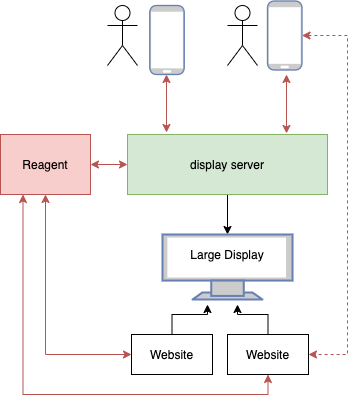
\includegraphics[width=0.8\columnwidth]{chapters/04_muifold/figures/muifold_architecture}
  \caption{Architecture of MUIFOLD. The red lines are WebSockets and the dotted line indicates an optional Web Socket depending on application needs.}
  \label{fig:architecture_muifold}
\end{figure}
\end{comment}

\subsection{Mobile Client}

The web-based mobile client, like other frameworks, is presented to the end-user through a simple webpage that the user opens on their
mobile device. This
can be either through scanning a QR code displayed on the large
display, or by manually typing in the URL. The client is
written using the React JS
framework~\footnote{https://reactjs.org/}, which provides a
high-level interface for building interactive UIs in JavaScript.
React provides a declarative language for the UI to be built in,
and helps to redraw the DOM as necessary as parts of the underlying
application state changes. Additionally, React allows us to define
the pieces of our UI as components, which makes it easy for us to
re-use pieces of the generic UI a user is greeted with when opening
the client in custom webview specific UIs as they need (e.g. like
for enabling pointing).
Out of the box, the mobile client presents the user with a generic
UI capable of interacting with any content displayed by the
large scale display, shown in Figure ~\ref{fig:mobile_start_ui}. The principle interaction methods in this
interface are pointing, left clicking, and scrolling content, similar
to the common mouse most users are familiar with from traditional
desktop and laptop computers.

\begin{figure}
\centering
  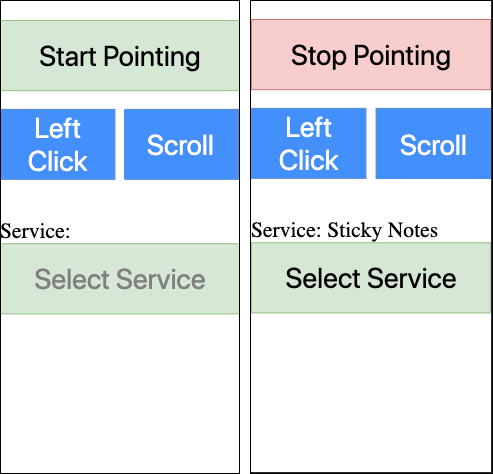
\includegraphics[width=0.65\columnwidth]{figures/generic_mobile_client}
  \caption{Generic interface for mobile client. Left view shows
  screen while not currently pointing. Right view shows client
  while actively pointing and cursor is over a display that has a custom application UI.}
  \label{fig:mobile_start_ui}
\end{figure}

Pointing is done through relative raycasting, relying solely
on the phone's builtin gyroscope and accelerometer and no additional
hardware through the DeviceOrientation API. When a user initially
connects, a
cursor is shown for the user at the center of the screen. Then,
while pointing is activated, for each tick the sensors report
their current degree, this is compared against the last measured
degree, taking the difference. This is then run through a smoothing
function~\cite{casiez_1_2012} to eliminate effects of natural
jitter, both in the sensors themselves and from slight hand
tremors. The client then reports this degree change to the display
server which translates this into a x,y pixel translation,
moving the cursor appropriately. The client then receives
information from the display server on if the cursor now is atop
a service that implements its own application specific UI. A
limitation of this approach is that over time, the cursor
eventually suffers from drift between where the user is pointing
to and where the cursor actually is. Self correction for this
though is easy enough by turning off pointing, re-adjusting
pointing position, and then turning back on pointing that it
this is not a great enough hindrance to ruin the approach. One thing
we did worry about was that as a user moved around the room and
interacted with the screen at different distances and angles, the
ratio of
degrees to pixels would need to change as well. In practice however,
we found that keeping this constant did not have any negative
effect on usage, so long as users stayed within 5-10 meters from
the ``sweet spot''.

Left clicking on the mobile interface is similar to how might
expect left-clicking with a standard mouse on a webview. Clicks that
happen within input fields, however will create a modal to appear
on the mobile interface that can be used to update that input
field, allowing the user to update the form in a mobile friendly
way. For example, clicking on a dropdown would show all of
the available options, clicking on an input would open the
keyborad, etc. Finally, when a user points at a webview that
is marked as having its own mobile UI, the button at the bottom
of the generic UI will activate with the name of the webview
appearing above it, such as in the right image in Figure
\ref{fig:mobile_start_ui}.

When opening a webview specific UI, the client gets the
URL for the webview's JavaScript to power its mobile UI. This
is then loaded dynamically, and injected into the running
application and run. It's expected that the JavaScript file will
either hook into the existing React root webview specific UIs or
can use vanilla JavaScript to build the DOM and manage it that way.
However, as stated above, with React, developers can utilize
components of the generic UI into their design as makes sense,
such as making available a button to toggle on / off pointing. The
only requirements for these UIs is that they must implement a button
that returns the user to the generic UI, and that they do not
overwrite the React root for the generic UI. Figure
\ref{fig:application_specific_ui} gives an example of how such
a UI might work for a specific application, in this case one
to create sticky notes. This UI re-uses the pointer component,
though shifted to the bottom of the screen, with custom content
for creating sticky notes. Hitting the ``Cancel'' button would
bring the user back to the generic UI.

\begin{figure}
\centering
  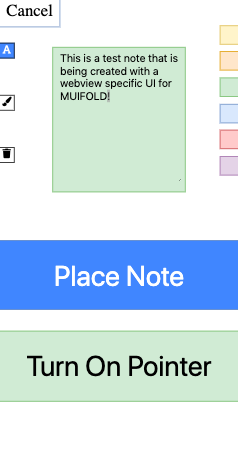
\includegraphics[width=0.40\columnwidth]{figures/application_specific_ui}
  \caption{Webview specific UI for a sticky notes application.}
  \label{fig:application_specific_ui}
\end{figure}


\section{User Study}

To determine the general effectiveness of our approach and that cellphones
would act as reliable pointing devices, we conducted a preliminary experiment.
Due to the nature of the experiment, we principally focused on qualitative
feedback from the participants over fully instrumenting out the experiment for
a range of measurements. \footnote{While a longer experiment with additional 
participants was planned, it was scrapped due to the COVID-19 lockdowns.}
For the experiment, we invited in members of IBM Brasil lab to use their phones 
to complete a test which utilized a variation of the Fitts' reciprocal tapping 
test~\cite{fitts_information_1954} and Liu et al.'s grid 
test~\cite{liu_effects_2014}.The hypothesis to be tested was that with minimal 
instruction, users would easily figure out the interface, and to complete the 
task quickly and efficiently.

\input{chapters/04_muifold/12_user_study/02_participants}

\input{chapters/04_muifold/12_user_study/03_hardware}

\input{chapters/04_muifold/12_user_study/05_tasks}

\input{chapters/04_muifold/12_user_study/07_surveys}

\input{chapters/04_muifold/12_user_study/09_results}

\input{chapters/04_muifold/12_user_study/12_discussion}

\section{Sample Use-Case}

\begin{figure}
\centering
  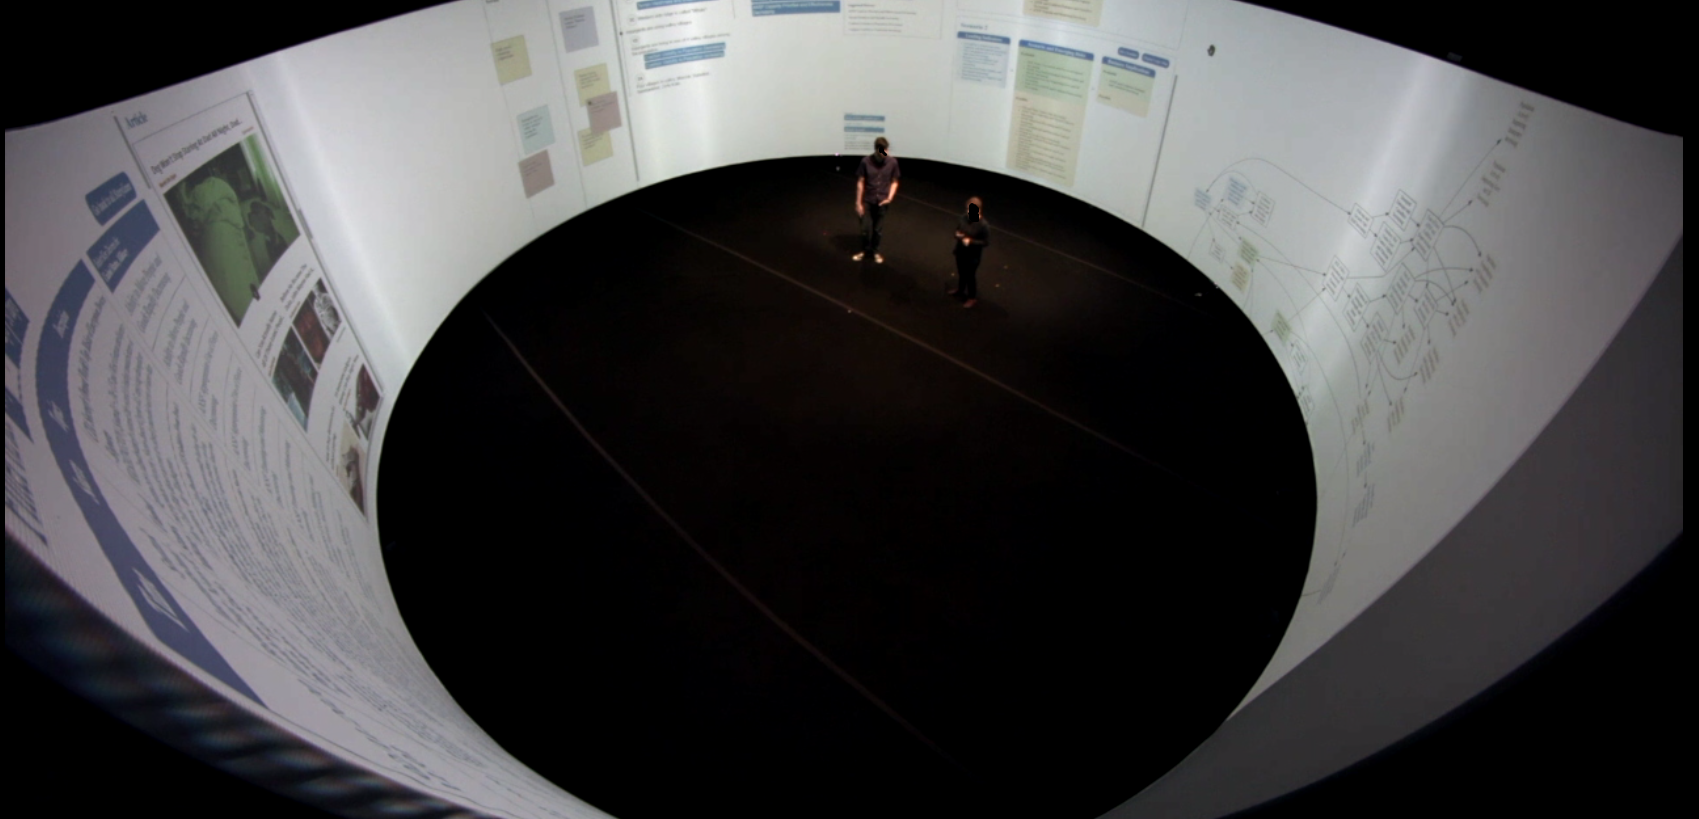
\includegraphics[width=0.8\columnwidth]{chapters/04_muifold/figures/demo_360.png}
  \caption{Overhead view of our use-case in the panoramic environment.}
  \label{fig:application_usecase}
\end{figure}

To demonstrate the effectiveness of our design, we created a sample
use-case centered around intelligence analysis, which brought together
multiple different applications into a single work-flow displayed
on a large 360° panaromic display, as shown in Figure~\ref{fig:application_usecase}~\footnote{A video of this demo 
use-case can be viewed at \url{https://www.dropbox.com/s/iokjvh0j6845688/iui_anonymous.mp4?dl=0}.}.
In this use-case, intelligent analysts are given a host of tools
to help them look at important news, create notes and hypothesises,
and generate ``what-if'' scenarios based on specific drivers they 
think could happen. For example, if the news talks about on-going
terrorist attacks within the Middle East, a driver they may select
would be ``Weakening of US and Allied Forces''.
Each piece of the application was implemented within its own webview 
open on the display server, and
where some utilized their own specific mobile UI, some did not. Each webview is always available to each user, and that they sit side-by-side to each other. We
briefly describe the different open webviews below. 

\subsection{Storyline Viewer}

This webview is composed of two parts. The first part gives a list
of ``storylines'', which is a grouping of articles pertaining to some
topic, like ``US, Military'' or ``Iraq, Trump''. This list can be
scrolled through, and clicking on a storyline will open up the list
of articles that are contained within that storyline. Clicking on an
article will then cause this view to issue a REST call to the display
server asking it to display the article's URL on the screen. There is
then a button to go back to the list of storylines, and clicking on
any column will cause the list to sort based on that column, first
ascending and then clicking again will cause it to be descending.
Currently, only one column will be sorted at a time. There is no
custom UI for the mobile application for this webview, however does
support left clicking and scrolling through the generic interface.

\subsection{Article Viewer}

As mentioned above, the Article Viewer is triggered by clicking on a
set article within the storyline viewer. This then triggers the
article to be loaded into its own set webview. These articles
come from various news organizations, such as the BBC, Reuters, etc.,
which we have no control over, but are still totally usable via our
generic interface, principally with scrolling through the article as well
being able to clicking on hyperlinks on the page to follow them.

\begin{figure}
\centering
    \hfill
    \subfigure[Storyline Viewer]{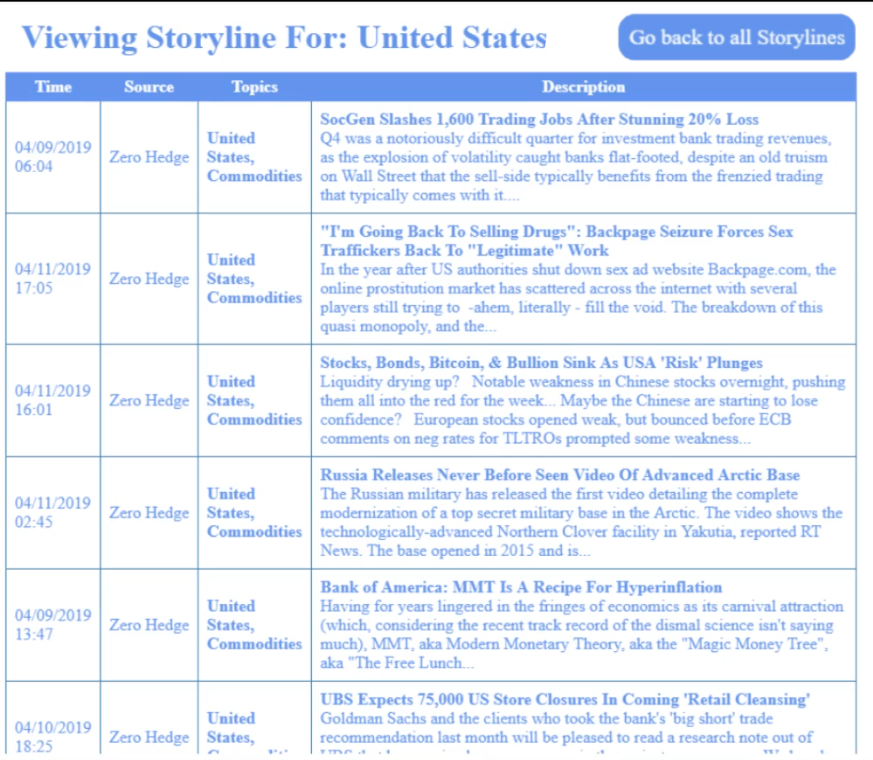
\includegraphics[width=0.3\columnwidth]{chapters/04_muifold/figures/storyline_viewer.png}}
    \hfill
    \subfigure[Article Viewer]{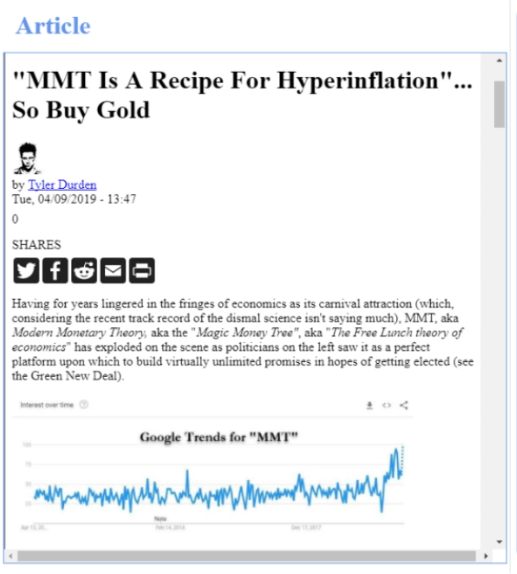
\includegraphics[width=0.25\columnwidth]{chapters/04_muifold/figures/article_viewer.png}}
    \hfill
    \\
    \hfill
    \subfigure[Scenario Generation Tool]{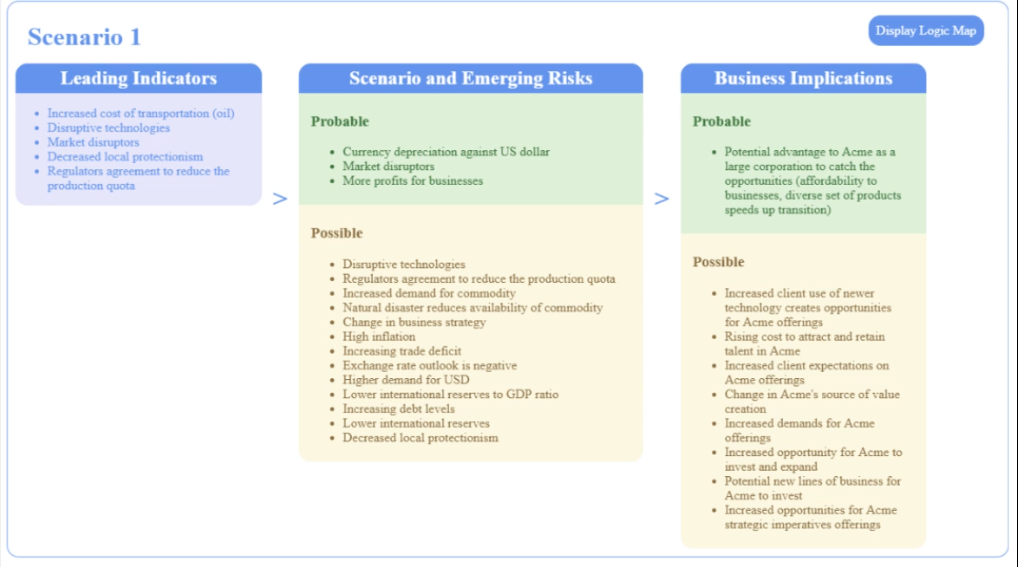
\includegraphics[width=0.4\columnwidth]{chapters/04_muifold/figures/scenario_planner.png}}
    \hfill
    \subfigure[Generated Scenario  Logic Map]{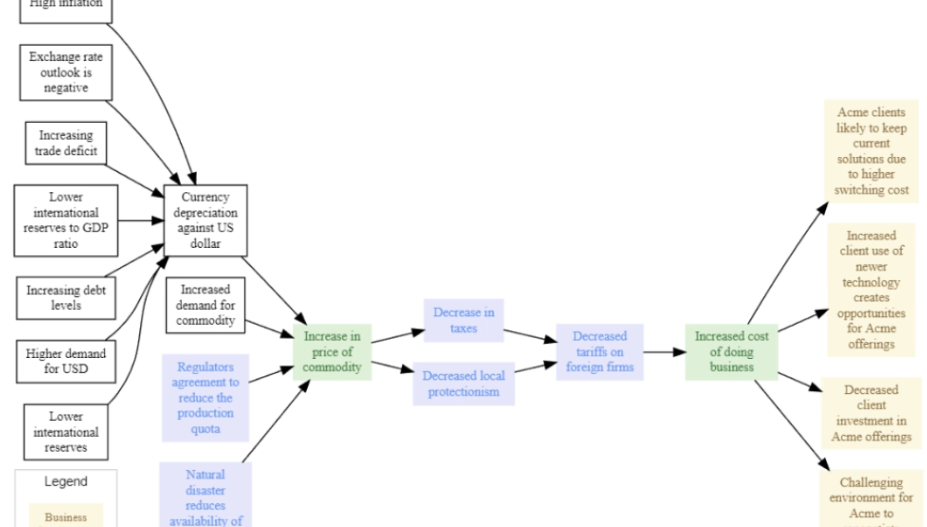
\includegraphics[width=0.4\columnwidth]{chapters/04_muifold/figures/scenario_planner_map.png}}
    \hfill
  \caption{Screenshots of different applications within the analyst use-case as shown on the large display.}
  \label{fig:muifold_use_case_grid}
\end{figure}

\subsection{Sticky Notes}

The webview containing the sticky note application is usable only
through a custom UI, triggered once a user moves their cursor
over the webveiw and clicks the button at the bottom of the generic
UI. They are then greeted with a screen allowing them to turn on / off
the cursor, when they move the their cursor over a note, they can
grab a note, create a note, and place notes currently loaded on the
phone. Figure \ref{fig:muifold_use_case_grid} gives a view of the
UI when a note is current being edited before being placed onto the
display. To handle interactions of notes between the phone and
webview, a WebSocket is opened specific to this application when
it is loaded on the client device. Once the client is finished with
this view, the WebSocket is closed.

\subsection{Prediction Creation Tool}

This webview contains predictions that are created by the analysts. Within our
environment, we provide space to create two hypothesises and to compare them
side-by-side. To utilize the tool, the analyst uses MUIFOLD to click on the
service on the large display. This opens an interface onto their phone where
they may write down the central prediction and then add as many minor supporting
predictions as they want. Under each supporting prediction, the user can then select
as many pieces of supporting evidence as they want, where each piece of evidence is
pulled from the sticky note application. The tool is shown in Figure~\ref{fig:prediction_ui}.

\subsection{Key Driver Selection Tool}

Key drivers are concepts of a scenario under analysis.
This tool provides usability in both the generic UI and also an
application specific UI for the client. Within the generic UI, a user
can left click on any previously selected driver to remove it
from the set under examination. Additionally, there is a dropdown
they can click to look at a list of all available drivers in the
system. This is shown in Figure ~\ref{fig:key_driver_tool}.
Alternatively, you can open an application specific UI on the client
which surfaces additional information, such as recently previously
selected drivers, drivers selected for previous scenarios, etc. that
would be not possible to display on the large display due to space
concerns.

\begin{figure}
\centering
    \hfill
    \subfigure[]{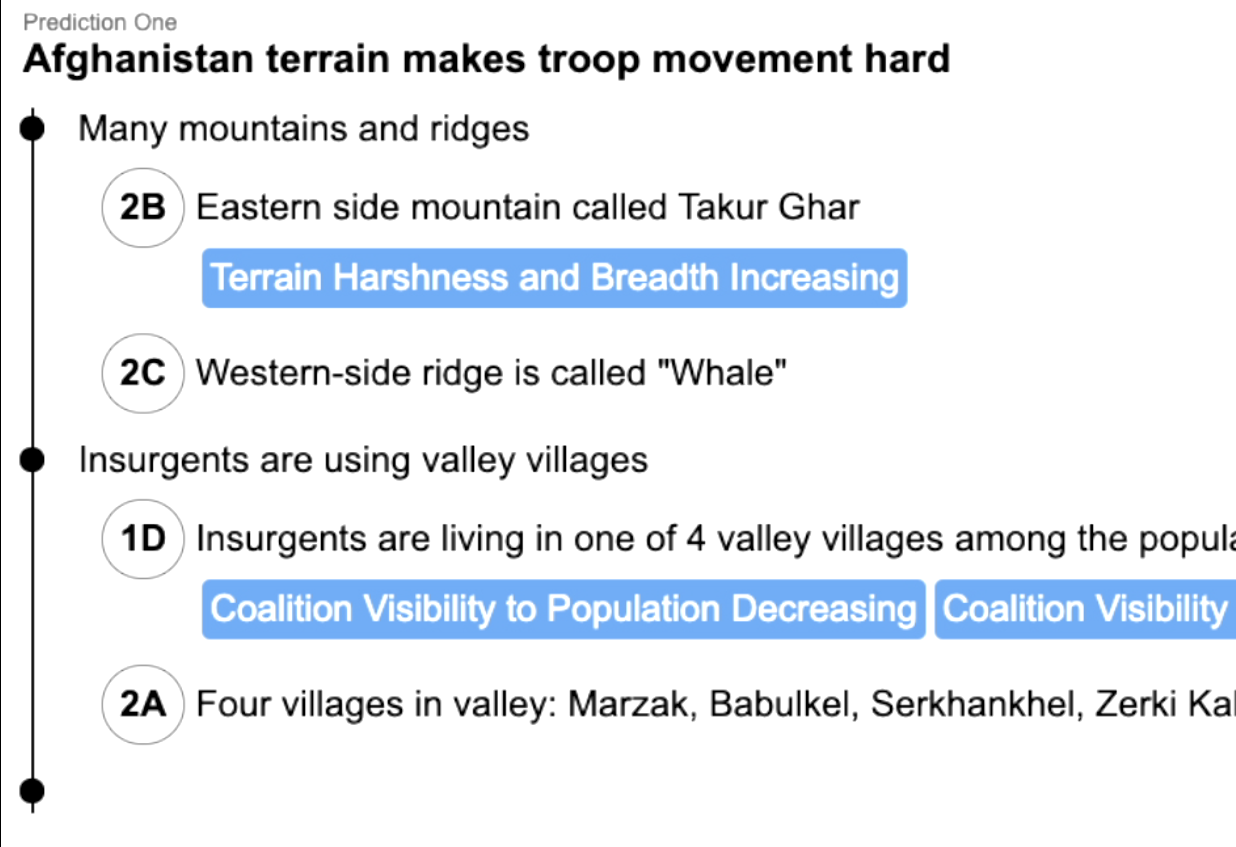
\includegraphics[width=0.5\columnwidth]{chapters/04_muifold/figures/hypthosis_generator.png}}
    \hfill
    \subfigure[]{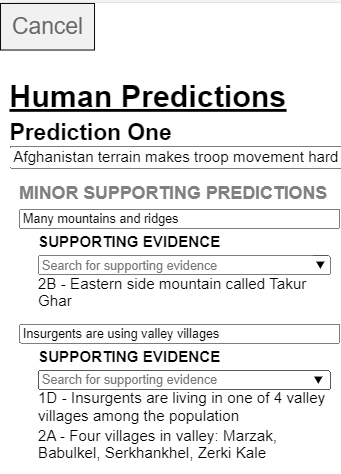
\includegraphics[width=0.25\columnwidth]{chapters/04_muifold/figures/hypthosis_muifold.png}}
    \hfill
  \caption{Screenshots of a) the hypothesis generation tool on the large display and b) its MUIFOLD interface.}
  \label{fig:prediction_ui}
\end{figure}

%\begin{figure}
%\centering
%  \includegraphics[width=0.4\columnwidth]{figures/mobile_ui_dropdown}
%  \caption{Generic UI with open dropdown.}
%  \label{fig:mobile_ui_dropdown}
%\end{figure}

\subsection{Scenario Generation}

After selecting drivers, a scenario is generated with a logic
map displayed using D3 and Graphviz, where showing the connections
between potential drivers that might have triggered or be triggered
by the selected drivers. Here, attempting to use the scroll detects
that the page itself cannot be scrolled, rather it can pan the D3
canvas, and so does that. Left clicking on a node in the graph
will trigger an event that either selects or deselects a driver. The
mobile specific UI here just mirrors down the graph to the personal
device, so a user can interact with it on their own. However, they can
lock the view of their personal device to that of the large display,
such that panning or zooming on the personal device will commit a
similar action on the large display. Communication here is done
through a websocket between the client and webview D3 instance,
where the zoom and pan coordinates are passed between the two, using
a fluid design for showing the content that fits the screen
real estate.

\begin{figure}
\centering
    \hfill
    \subfigure[]{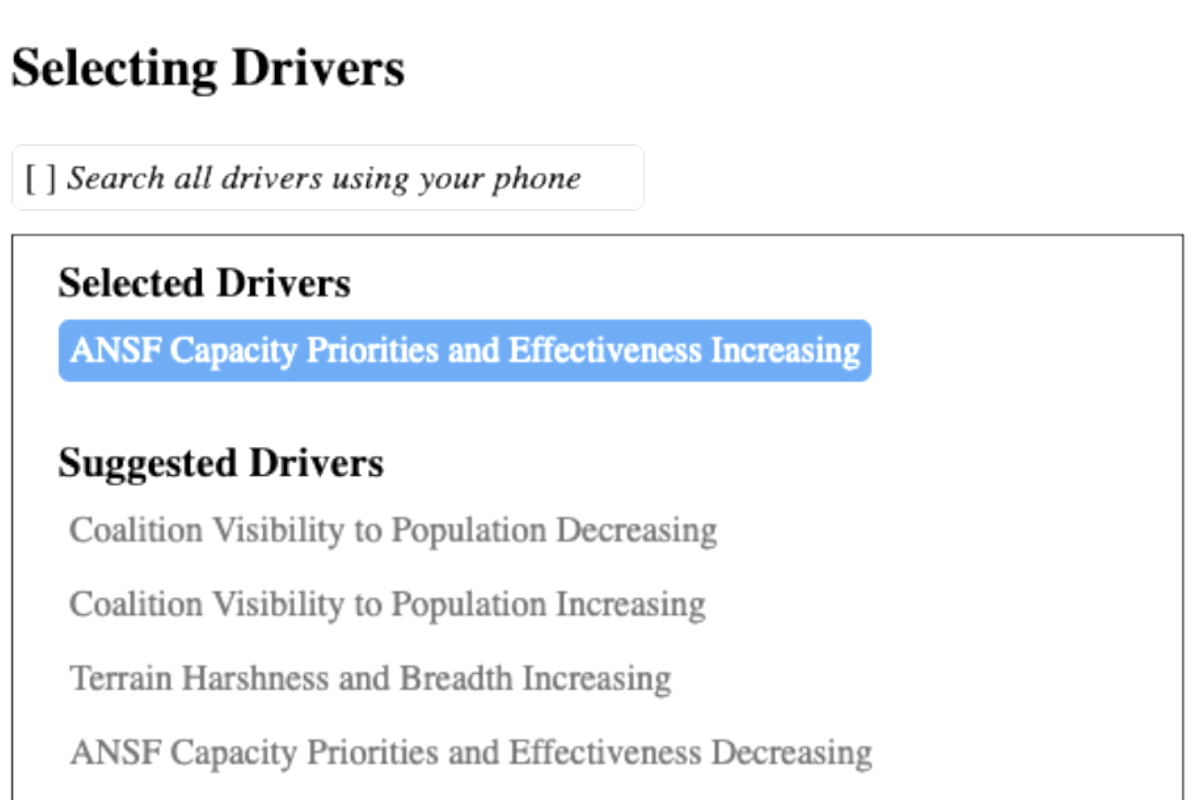
\includegraphics[width=0.5\columnwidth]{chapters/04_muifold/figures/driver_select_screen.png}}
    \hfill
    \subfigure[]{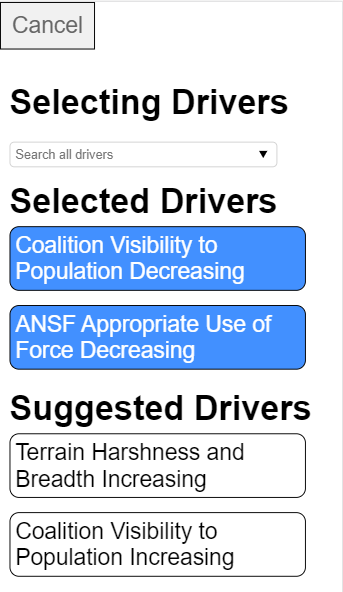
\includegraphics[width=0.25\columnwidth]{chapters/04_muifold/figures/driver_select_muifold.png}}
    \hfill
  \caption{Screenshots of a) the driver selection tool on the large display and b) its MUIFOLD interface.}
  \label{fig:key_driver_tool}
\end{figure}

\section{Discussion of Limitations}\label{chap04:limitations}

In this section, we provide some lessons learned about certain
aspects of the technology from our preliminary user study and
sample use-case.

\textbf{Location and Size of UI Buttons} One of the biggest design challenges
was dealing with placement of
buttons for the generic UI, as well as general guidelines for the
developers of webview specific UIs. The principle goal was that
users of the system, after some practice, would be able to use
their phones and the buttons on it without having to look down
at it. This was accomplished in three ways. First, buttons we expect a
user to use without looking down are centered around the middle
$\frac{1}{3}$ of the screen. This corresponds to the average rotation
of our user's thumb when naturally holding their devices. Second,
each button was given a large dimensions to make it harder to ``fat
finger'' a wrong button without looking. Thirdly, we provide haptic
feedback through quick phone vibrations whenever a user clicks a
button, allowing them to know that they hit it. Unfortunately, we
found during implementation that haptic feedback was only available
to android users.

\textbf{Permissions} To utilize many of the underlying sensors or
capabilities of the phone in a web context, permissions are frequently
asked, such as if attempting to use location, use the camera, etc. However,
due to historical reasons, this is not true for the DeviceOrientation
API on most devices which we rely on for determining where the phone
is pointing at. Many users found this somewhat disconcerting. We
found that users would feel more comfortable if we showed a fake
permissions prompt asking users if we could utilize the gyroscope
and accelerometer. Interestingly, while developing the framework,
iOS 13 was released which actually does require users to give
permission to use the sensors, but this is done through system
settings, which some users found a bit confusing if not provided
step-by-step instructions. However, in using React, we can utilize
the ReactNative library to generate native apps that do not have
these issues, at the cost of requiring the user to download and install
the app.

\textbf{Providing ``Fluid'' UIs} Among our 10 subjects, very few shared
the same phone model, and each had a different amount of
available screen real estate. To handle such differences,
there's a paradigm of ``fluid'' layout according to which the content
dimensions are based on percentages of available screen real estate. This
allowed us to deal with the size differences. Unfortunately, when
opening the keyboard on both iOS and android, the screen size as
reported to the page changes, causing the content to become messed up
in location and size. To overcome this, when loading our client
application, we implement a two-stage loading process. In the
first phase, we load the content relative to the size of the screen.
In the second phase, we sweep over all elements and provide them
fixed sizes and positions. Luckily, it is easy to detect screen
rotation to re-draw all elements as necessary, but we do not need to
worry about the screen size otherwise changing.

\textbf{Browser and Device Incompatibilities} The biggest challenge
we faced was in slight browser incompatibilities across a range of
devices. The first is that each browser provides a different frame
of reference for the coordinate system used by the DeviceOrientation
API. For example, Firefox and Chrome browsers on the same device would
consistently report angles that were 20$\deg$ apart. Additionally,
refreshing the open page might cause the sensors to ``reset'' and report
a completely new angle. Finally, on certain devices, the browsers
would report the orientation in an opposite direction from the way
the phone was rotating, causing the cursor to go in the opposite
direction. There did not happen on specific browsers regardless of
device, so the solution was to provide a user with a setting to
flip orientation tracking to correct it.


\section{Summary}

In this chapter, we laid out and demonstrated MUIFOLD, a novel
framework for building out mobile interfaces for interaction
with our CAIS, namely in the context of large displays. The principal
contribution of this framework, compared to prior work, is its
ability to work across a wide range of websites, both first party
and third party, out of the box, while providing easy extension points
for building out custom UIs for a given site. This was demonstrated
in a sample use-case for intelligence analysts that utilized a mix
of third-party and first-party content, and which some screens
utilizing a custom UI and others not. However, of equal importance is
that our approach by utilizing the builtin sensors of a cellphone
and relying on a method of relative ray-casting allowed our technology
to be used immediately in new environments without the costly or
difficult steps of calibration as seen in other approaches that utilized
more precise external sensors or devices. We also provided an initial
user study to evaluate the basics of the technology, namely on the
reliability of the pointing, and ability of the users to be able to select
and manipulate content on the screen. While our results were below
that of prior work, we identified several ways in which we may boost
our results in follow-up work. However, perhaps more importantly is that
what we lose in pointing accuracy, is more than made up on in the increased
amount of interactions that are possible by utilizing the phone's screen
for displaying content to the user from the large screen.


% 4. Formalizing the CAIS
\chapter{Formalizing the CAIS}\label{chap:formalizing}

\section{Introduction}

Now that we have established both a framework for building out a CAIS and
a practical implementation, in this chapter we now establish the formal
schematics for our framework that we informally defined above. To accomplish
this, we require a highly expressive language capable of modeling agents'
cognitive states, including beliefs, knowledge, etc. These cognitive states
can range over physical details of the world at large, or even about the
cognitive states of other agents.

To accomplish this task, we introduce the \textit{Cognitive Event
Calculus} (\CEC), which is a highly expressive intentional logic that fits
our needs. We briefly provide a definition of the logic, and an description
of its syntax and sorts. Additionally, we briefly cover how we can handle
the logic in an automated fashion using ShadowProver. From this, we then
provide a formalization of the principles of a CAIS, and for how fundamenta
actions (such as pointing) are captured from the CAIS into the \CEC. We
close out the chapter tying together these efforts in demonstration of
solving a psychological test by the CAIS to demonstrate its capacity
for dealing with theory-of-mind reasoning.

%    1. Deontic Cognitive Event Calculus
%        1. ShadowProver
%        2. Spectra
\section{The Cognitive Event Calculus}

%TODO:
%   1. go through and expand CEC
%   2. remove duplicate tables of syntax/sorts
%   3. Add subsection on shadowprover

To capture the CAIS in a formal way, we employ the
\textbf{cognitive event calculus} (\CEC), a cognitive calculus and
intensional logic, which provides a subset of the \DCEC~\cite{nsg_sb_dde_ijcai}
\footnote{For a richer primer on the \DCEC, we invite users to view the
appendix of that work}. The \CEC\ is a multi-sorted quantified modal logic with a 
well-defined syntax and proof calculus. The use of sorts here can be thought of
as being analogous to a typed single-inheritance programming language. The
proof calculus of \CEC\ is based on natural deduction 
\cite{gentzen_investigations_1964} and includes all the introduction and
elimination rules for first-order logic, as well as inference schemata for
the modal operators and related structures discussed below. At its core, the
\CEC\ subsumes the event calculus~\cite{mueller_commonsense_2014} (EC), a
first-order calculus used for
modeling events and actions and their effects upon the world. The modal
operators that the \CEC\ adds on top of the EC are that
$\believes$elief, $\knows$nowledge, $\common$ommon Knowledge, $\perceives$erceiving,
$\says$aying, $\desires$esiring, and $\intends$ntending. At a surface level,
the \CEC\ may appear similar to readers to BDI logics~\cite{rao_modeling_1991},
but  differ in a number of key ways. The most significant is that BDI logics
utilizes \textit{possisble-worlds semantics} with uninstantiated inference
schema, but rather utilizes \textit{proof-theoretic sematics} as it is based
on natural deduction~\cite{gentzen_untersuchungen_1935}\footnote{Bringsjord and
Govindarajulu~\cite{bringsjord_given_2012} provide a deeper explanation for
the interested reader.}. Additionally, through the inclusion of operators
like perception, communication, and intensional operators, the \CEC\ aims
to facilitate ease of use within fields of computer vision and natural language.

\begin{table}
\begin{footnotesize}
\begin{center}
\begin{tabular}{lp{8cm}}
\toprule
\textbf{Sort}    & \textbf{Description} \\
\midrule
\type{Agent} & Human and non-human actors.  \\

\type{Moment} &  Time points. E.g., $t_i$, $birthday(son(jack))$ etc. \\

  \type{Event} & Used for events in the domain. \\
  \type{ActionType} & Abstract actions
                      instantiated by agents.\\
  \type{Action} & Events that occur
                  as actions by agents \\
  \type{Fluent} & Representing states of the world.\\
  \type{Formula} & Represents any arbitrary formula\\
  \bottomrule
\end{tabular}
\caption{Basic sorts in the language}
\label{table:sorts}
\end{center}
\end{footnotesize}
\end{table}

\begin{figure}[ht]
% frametitle=Signature (snippet), 
\begin{mdframed}[roundcorner=8pt, nobreak=true, frametitlealignment=\centering]
\begin{equation*}
 \begin{aligned}
    \mathit{S} &::= 
    \left\{\begin{aligned}
      & \Object \sep \Agent  \sep \ActionType \sep \Action \sqsubseteq
      \Event \sep \\ &\Moment  \sep \Fluent \sep \Numeric\\
    \end{aligned} \right.
    \\ 
    \hspace{-29pt}\mathit{f} &::= \left\{
    \begin{aligned}
      & \action: \Agent \times \ActionType \rightarrow \Action \\
      &  \initially: \Fluent \rightarrow \Boolean\\
      &  \holds: \Fluent \times \Moment \rightarrow \Boolean \\
      & \happens: \Event \times \Moment \rightarrow \Boolean \\
      & \clipped: \Moment \times \Fluent \times \Moment \rightarrow \Boolean \\
      & \initiates: \Event \times \Fluent \times \Moment \rightarrow \Boolean\\
%      & \terminates: \Event \times \Fluent \times \Moment \rightarrow \Boolean \\
      & \prior: \Moment \times \Moment \rightarrow \Boolean\\
    \end{aligned}\right.\\
        \mathit{t} &::=
    \begin{aligned}
      \mathit{x : S} \sep \mathit{c : S} \sep f(t_1,\ldots,t_n)
    \end{aligned}
    \\ 
    \mathit{\phi}&::= \left\{ 
    \begin{aligned}
     & 
        A(\ldots):\Boolean \sep 
        \neg \phi \sep
        \phi \land \psi \sep
        \phi \lor \psi \sep \\
    &
        \phi \lif \psi \sep
        \phi \liff \psi \sep
        \exists x \phi(x) \sep
        \forall x \phi(x)\\
     &
        \perceives (a,t,\phi)  \sep
        \knows(a,t,\phi) \sep
        \common(t,\phi) \sep
        \believes(a,t,\phi) \\
    &
        \says(a,t,\phi) \sep
        \says(a,b,t,\phi)  \sep
        \desires(a,t,\phi) \sep
        \intends(a,t,\phi) \\
      \end{aligned}\right.
  \end{aligned}
\end{equation*}
\end{mdframed}
\caption{\CEC\ Syntax}
\label{fig:cec_syntax}
\end{figure}

We know provide a brief primer on the event calculus and \CEC\ to make
accessible the following chapter. The sorts of our logic are shown in 
Table~\ref{table:sorts}. Most of the sorts shown come from the underlying EC,
but we add here three additional sorts: \Agent, \Action, and \ActionType.
The syntax of the \CEC\ is shown in Figure~\ref{fig:cec_syntax}. In our
syntax, the symbols of the event calculus are contained under $\mathit{f}$.
An important axiom that drives much of the event calculus is:
\vspace{-0.4cm}
\begin{equation*}
    \begin{aligned}
        \happens(e, t_{1}) \land \initiates(e, f, t_{1}) \land (t_{1} < t) \land \lnot\clipped(t_{1}, f, t) \rightarrow \holds(f, t)
    \end{aligned}
\end{equation*}

\noindent
which can be read as "some event $e$ \happens at time $t_{1}$ and that this $e$
\initiates our fluent $f$ at $t_1$ such that at some later time $t$, and assuming
that there has not been something causing $f$ to be \clipped (made false) between
$t_{1}$ and $t$, then $f$ holds at time $t$". From this axiom, we see that the
event calculus is non-monotonic, such that fluents can hold at some time, but
not hold at other times, and that this is determined by the events of the
system at large.

On top of this, as part of the allowed functions and relations to the system,
shown as $\mathit{\phi}$, we add the intensional operators which can be read as:
\perceives\ is an agent $a$ at time $t$ perceives $\mathit{\phi}$, \knows\
is an agent at time $t$ knows $\mathit{\phi}$, \common\ is at time $t$ that
$\mathit{\phi}$ is common knowledge to all agents, \believes\ is
an agent $a$ at time $t$ believes $\mathit{\phi}$ at time $t$, \says\ is
agent $a$ at time $t$ says $\mathit{\phi}$ or that agent $a$ at time $t$
says $\mathit{\phi}$ to agent $b$, \desires\ is agent $a$ at time $t$ desires
$\mathit{\phi}$, and \intends\ is agent $a$ at time $t$ intends $\mathit{\phi}$.
With our syntax established, we now move to the inference schemata, shown in
Figure~\ref{fig:cec_schemata}.

\begin{figure}[h]
% frametitle=Inference Schemata (snippet),
\begin{mdframed}[nobreak=true, roundcorner=8pt, frametitlealignment=\centering]
\begin{equation*}
\begin{aligned}
% &\mbox{Sample rules below. For more rules, see
%   \cite{akratic_robots_ieee_n}.}\\
  &\infer[{[R_{\knows}]}]{\knows(a,t_2,\phi)}{\knows(a,t_1,\Gamma), \ 
    \ \Gamma\vdash\phi, \ \ t_1 \leq t_2} \\ 
& \infer[{[R_{\believes}]}]{\believes(a,t_2,\phi)}{\believes(a,t_1,\Gamma), \ 
    \ \Gamma\vdash\phi, \ \ t_1 \leq t_2} \\
& \infer[{[R_1]}]{\common(t,\perceives(a,t,\phi) \lif\knows(a,t,\phi))}{}\\
&  \infer[{[R_2]}]{\common(t,\knows(a,t,\phi)
    \lif\believes(a,t,\phi))}{}\\
  &\infer[{[R_3]}]{\knows(a_1, t_1, \ldots
    \knows(a_n,t_n,\phi)\ldots)}{\common(t,\phi) \ t\leq t_1 \ldots t\leq
    t_n}\hspace{10pt}
  \infer[{[R_4]}]{\phi}{\knows(a,t,\phi)}\\
  & \infer[{[R_5]}]{\common(t,\knows(a,t_1,\phi_1\lif\phi_2))
    \lif \knows(a,t_2,\phi_1) \lif \knows(a,t_3,\phi_2)}{}\\
& \infer[{[R_6]}]{\common(t,\believes(a,t_1,\phi_1\lif\phi_2))
    \lif \believes(a,t_2,\phi_1) \lif \believes(a,t_3,\phi_2)}{}\\
& \infer[{[R_7]}]{\common(t,\common(t_1,\phi_1\lif\phi_2))
    \lif \common(t_2,\phi_1) \lif \common(t_3,\phi_2)}{} \\
& \infer[{[R_8]}]{\common(t, \forall x. \  \phi \lif \phi[x\mapsto
  t])}{} \\
& \infer[{[R_9]}]{\common(t,\phi_1 \liff \phi_2 \lif \neg
    \phi_2 \lif \neg \phi_1)}{}\\
& \infer[{[R_{10}]}] {\common(t,[\phi_1\land\ldots\land\phi_n\lif\phi]
  \lif [\phi_1\lif\ldots\lif\phi_n\lif\psi])}{}\\
% & \infer[{[R_{11a}]}]{\believes(a,t,\psi)}{\believes(a,t,\phi)\ \ \phi
%   \lif \psi}\
%\hspace{6pt} \infer[{[R_{11b}]}]{\believes(a,t,\psi \land \phi)}{\believes(a,t,\phi)\ \ \believes(a,t,\psi)}\\ 
& \infer[{[R_{12}]}]{\believes(h,t,\believes(s,t,\phi))}{\says(s,h,t,\phi)} \\
& \infer[{[R_{13}]}]{\perceives(a,t,\happens(\action(a^\ast,\alpha),t))}{\intends(a,t,\happens(\action(a^\ast,\alpha),t'))}
\end{aligned}
\end{equation*}
\end{mdframed}
%\end{scriptsize}
\caption{\CEC\ Inference Schemata}
\label{fig:cec_schemata}
\end{figure}

$R_\mathbf{K}$ and $R_\mathbf{B}$ state that for knowledge and belief, if an
agent knows or believes some formula $\Gamma$ at time $t_{1}$, and that $\Gamma$
entails some formula $\phi$, then at some equal or later time $t_{2}$, the
agent will know or belief the formula $\phi$. Under these two rules, it
establishes that knowledge and belief are closed under the inference system of
\CEC. $R_{1}$ and $R_{2}$ state that it is common knowledge that perception
leads to knowledge and that knowledge to belief respectively. $R_{3}$ states that
any formula that is common knowledge, all agents know that formula, and also know
that all other agents know that formula, iteratively. $R_{4}$ states that
knowledge  of a formula implies that that formula holds. Through the use of
$R_{3}$ and $R_{4}$, we can unwind any formula that is common knowledge, such
as for $R_1$, we could derive
$\perceives(a, t, \phi) \rightarrow \knows(a, t, \phi)$. $R_5$ to $R_{10}$
provide for a more restricted form of reasoning for propositions that are common
knowledge, unlike propositions that are known or believed.  $R_{12}$
states that if an agent $s$ communicates a proposition $\phi$ to $h$,
then $h$ believes that $s$ believes $\phi$. $R_{13}$ states that for for some
action that agent $a$ intends action $\alpha$, then they will perceive that they
perceive that action at a different time. For our work here, $R_{1}$ to $R_{4}$
and $R_{12}$ are most important for our formalization and reasoning efforts.
To utilize our logic as part of the CAIS, past the formalization, we utilize
an automated theory prover, \textsf{ShadowProver}, which is described in greater
detail in section~\ref{sec:automated_reasoner_planner}.


%    2. Formalization of Requirements
\section{Formalizing the Requirements for a CAIS}\label{sec:formalization_cais}

It should be noted that a CAIS to be considered a truly ``intelligent''
room, it is not sufficient that the room be intelligent about, for
example, search queries over a domain $D$; the room should also be
intelligent about cognitive states of agents in the room and their
cognitive states towards $D$.

Despite there being a significant amount of work done in building
intelligent environments (of varying levels of intelligence;
\cite{coen_design_1998, brooks_intelligent_1997,chan_review_2008}), there
is no formalization of what constitutes an intelligent room and what
separates it from an intelligent agent.  Though \cite{coen_design_1998}
briefly differentiates an intelligent room from ubiquitous computing
based on the non-ubiquity of sensors in the former, there is not any
formal or rigorous discussion of what separates an intelligent room
from a mobile robot that roams around the room with an array of
sensors.  We offer below a sketch of informal requirements that an
immersive room should aim for.  Then we instantiate these requirements
using \CEC.

Assuming that these two conditions hold, we can use them to make determinations
about the properties of such systems, as well as to help distinguish the various
classes of intelligent rooms and their capabilities that have been historically created.
%\subsection{Formal Requirements for a CAIS}
%\label{sect:freqs}
From the information requirements, we look to translate them into a formalized 
version for a CAIS. The formal requirements are explained below:

    \begin{mdframed}[frametitle= Formal Requirements for $\mathcal{C}$ ,
      frametitlebackgroundcolor=gray!25, nobreak,
      linecolor=white,backgroundcolor=gray!10]
      Assume $\Gamma \vdash t < t + \Delta$
      \begin{enumerate}
      \item[$\mathbf{C}^f_1:$] It is common knowledge that, if an
        agent $x$ has a false belief, $\gamma$ informs the agent of
        the belief:\footnote{Please note that inference in \CEC\ is
          non-monotonic as it includes the event calculus, which is
          non-monotonic.  If an agent $a$ believes $\phi$ based on
          prior information, adding new information can cause the
          agent to not believe $\phi$.}
         \begin{equation*}
          \common\color{gray!80}\left(\color{black}t, \left[\begin{aligned}
                &  \believes(\gamma, t, \phi) \land \believes(\gamma, t,
                \believes\big(x, t, \lnot \phi)\big)
                \\ & \hspace{50pt} \rightarrow \\
                & \hspace{30pt}\says(\gamma, x, t + \Delta, \phi)
              \end{aligned}\right]\color{gray!80}\right)\color{black}
        \end{equation*}

      \item[$\mathbf{C}^f_2:$] It is common knowledge that, if an
        agent $x$ has a missing belief, $\gamma$ informs the agent of
        the belief:
        \begin{equation*}
          \common\color{gray!80}\left(\color{black}t,\left[ \begin{aligned}
                &  \believes(\gamma, t, \phi) \land \believes(\gamma, t,
                \lnot \believes\big(x, t, \phi)\big)
                \\ &  \hspace{50pt}  \rightarrow \\
                & \hspace{30pt}\says(\gamma, x, t + \Delta, \phi)
              \end{aligned}\right]\color{gray!80}\right)\color{black}
        \end{equation*} \end{enumerate}
    \end{mdframed}
    
\begin{mdframed}[frametitle= Formal Requirements for $\mathcal{I}$ ,
  frametitlebackgroundcolor=gray!25, nobreak,
  linecolor=white,backgroundcolor=gray!10]
  \begin{enumerate}
  \item[$\mathbf{I}^f_1:$] It is common knowledge that at any
    point in time $t$ an agent $x$, different from the CAIS system
    $\gamma$, can observe events or conditions (fluents) only in
    its vicinity.
    \begin{equation*}
      \begin{aligned}
        \common\Bigg(\forall x, t, f:& (x \not = \gamma) \rightarrow \Big[\perceives\big(x, t, \holds(f, t)\big) \rightarrow
        \holds(\vicinity(x, f), t)\Big]\Bigg)\\
        \common\Bigg(\forall x, t, e:& (x \not = \gamma) \rightarrow \Big[\perceives\big(x, t, \happens(e, t)\big) \rightarrow
        \holds(\vicinity(x, e), t)\Big]\Bigg)\\
      \end{aligned}
    \end{equation*}

  \item[$\mathbf{I}^f_2:$] It is common knowledge that actions
    performed by the agent are in its vicinity.
    \begin{equation*}
      \common\Big(\forall x, \alpha:  \holds\big(\vicinity(x, \action(a, \alpha)), t\big)\Big)
    \end{equation*}
  \item[$\mathbf{I}^f_3:$] It is common knowledge that all events
    and fluents are perceived by $\gamma$.  This is represented by
    the four conditions below:
    \begin{equation*}
      \begin{aligned}
   &  (i) \hspace{10pt}  \common\Bigg(\forall  t, f:  \Big[\holds(f, t) \leftrightarrow \perceives\big(\gamma, t, \holds(f, t)\big) \Big]\Bigg)\\
   & (ii)  \hspace{10pt}   \common\Bigg(\forall  t, e: \Big[\happens(e, t)
        \leftrightarrow \perceives\big(\gamma, t, \happens(e,
        t)\big) \Big]\Bigg)\\
    &   (iii)  \hspace{10pt}   \common\Bigg(\forall  t, f:  \Big[\lnot \holds(f, t)
        \leftrightarrow \perceives\big(\gamma, t, \lnot \holds(f, t)\big) \Big]\Bigg)\\
    &   (iv) \hspace{10pt}    \common\Bigg(\forall  t, e:\Big[\lnot \happens(e, t)
        \leftrightarrow \perceives\big(\gamma, t, \lnot \happens(e, t)\big) \Big]\Bigg)
      \end{aligned}
    \end{equation*}
  \end{enumerate}
\end{mdframed}

Time is assumed to be discrete, as in the
discrete event calculus presented in \cite{mueller_commonsense_2014}.  There is a
background set of axioms and propositions $\Gamma(t)$ that is
operational at time $t$.  We have a fluent $\vicinity$ that tells us
whether an agent is in the vicinity of a fluent, event, or another
agent:

$$\vicinity: \Agent \times \Fluent \cup \Event \cup \Agent \rightarrow
\Fluent $$

\noindent
Only events and fluents in the vicinity of an agent can be
observed by the agent.


One of the benefits of having a properly formalized CAIS is that we
can now state and prove various properties about these systems. If such
a system satisfies the above requirements, we can derive a foundationally
important (object-level in \CEC) property that we call:

\begin{small}
\begin{mdframed}[linecolor=white, frametitle=Expectation of Usefulness , frametitlebackgroundcolor=gray!25,
  backgroundcolor=gray!10, nobreak=true ,roundcorner=8pt]
  If the above properties hold, then an agent $a$ that perceives that
  another agent $b$ is not aware of an event happening, believes that
  CAIS $\gamma$ will inform $b$ (Assume: $\Gamma \vdash t < t + \Delta$):
\begin{equation*}
\begin{aligned}
&\perceives\big(a, t, \happens\big(e, t\big)\big) \land \perceives\Big(a, t, \lnot \holds\big(\vicinity(b, e),t\big)\Big) \\
& \hspace{90pt} \rightarrow \\
& \hspace{30pt} \believes\Big(a, t, \says\big(\gamma, b, t +\Delta,
\happens(e, t)\big)\Big)\\
\end{aligned}
\end{equation*}
\end{mdframed}
\end{small}

Through this property, humans within a CAIS can rely upon it to help other
agents with relevant missing or false information $\phi$, as opposed to the
case with a mobile robot. If we had a localized mobile robot instead of the
CAIS which failed to meet the above formal requirements, and therefore lacked
the above property, the human would need to decide whether or not the robot has
the required information $\phi$ and needs to believe that the robot believes that
another agent is missing the relevant information $\phi$. To help illustrate this
point, we provide a proof sketch using the inference schema of the \CEC\ and
the above formal requirements to derive the property:\footnote{We add color here
to ease reading of the proof, and for tracing terms through.}

%\noindent{\textbf{Proof Sketch}}: 


\begin{footnotesize} 
    \begin{prooftree}
      \AxiomC{$\perceives(a, t, \happens(e, t))$}
      \LeftLabel{$D_{[\perceives \leadsto \knows]}$}   \UnaryInfC{$\knows(a, t, \happens(e, t))$}        
     \LeftLabel{$D_{[\knows \leadsto \believes]}$}     \UnaryInfC{$\believes(a, t, \happens(e, t)) \equiv \boxed{\phi_1}$}   
  \end{prooftree}

    \begin{prooftree}
      \AxiomC{$\perceives(a, t, \lnot \holds\big(\vicinity(b, e),t\big))$}
   \LeftLabel{$D_{[\perceives \leadsto \knows]}$}   \UnaryInfC{$\knows\Big(a, t, \lnot \holds\big(\vicinity(b, e),t\big)\Big)$}        
     \LeftLabel{$D_{[\knows \leadsto \believes]}$}    \UnaryInfC{$\believes\Big(a, t, \lnot \holds\big(\vicinity(b, e),t\big)\Big) \equiv \boxed{\phi_2}$}   
  \end{prooftree}
\end{footnotesize}

Using $\mathbf{I}^f_3(ii)$ the CAIS observes all events that happen in
its enclosure:
\begin{footnotesize} 
\begin{prooftree}
        \AxiomC{$\mathbf{I}^f_3 (ii) \equiv\common\Bigg(\forall t, e: \Big[\happens(e, t) \leftrightarrow \perceives\big(\gamma, t, \happens(e, t)\big) \Big]\Bigg)$}
    \LeftLabel{$D_{[\common \leadsto \believes]}$  }
    \UnaryInfC{$\believes\left(a, t, \forall t, e: \Big[\happens(e, t)
            \leftrightarrow \perceives\big(\gamma, t, \happens(f, t)\big)
            \Big]\right)$}    \AxiomC{$\boxed{\phi_1}$}    
     \LeftLabel{$R_{\mathbf{B}}$}   \BinaryInfC{$\believes\Big(a, t, \perceives\big(\gamma, t,
          \happens(e, t)\big)\Big)$}   
      \LeftLabel{$R_{\mathbf{B}}$}  \UnaryInfC{$\believes \color{black}\big(\color{black} a, t, \color{violet}\believes\big(\gamma, t, \happens(e,t)\big) \color{black}\big)\color{black} \equiv
   \boxed{\psi_1}$}   
\end{prooftree}
\end{footnotesize} 
Similarly, using $\mathbf{I}^f_3 (iii)$:
\begin{footnotesize} 
\begin{prooftree}
        \AxiomC{$\mathbf{I}^f_3 (iii) \equiv \common\Bigg(\forall t,e : \Big[\lnot
          \holds(e, t)\leftrightarrow 
          \perceives\big(\gamma, t,  \lnot
          \holds(e, t)\big) \Big]\Bigg)$}
    \LeftLabel{$D_{[\common \leadsto \believes]}$  }  
\UnaryInfC{$\believes\left(a, t,\forall t, e\Big[\lnot
          \holds(e,t)\leftrightarrow 
          \perceives\big(\gamma, t,  \lnot
          \holds(e, t)\big)\Big]\right)$}        
\AxiomC{$\boxed{\phi_2}$} 
     \LeftLabel{$R_{\mathbf{B}}$}   \BinaryInfC{$\believes(a, t,
       \perceives(\gamma, t, \lnot 
          \holds\big(\vicinity(b, e), t)))$}   
    \LeftLabel{$R_{\mathbf{B}}$}     \UnaryInfC{$\believes(a, t,
      \believes\big(\gamma, t,  \lnot \holds\big(\vicinity(b, e), t\big))
      \equiv \boxed{\phi_3}$}   
\end{prooftree}
\end{footnotesize} 
From $\mathbf{I}^f_1$ (and from $\believes\big(a, t, \believes(\gamma, t, b \not = \gamma))$):
\begin{footnotesize} 
\begin{prooftree}
        \AxiomC{$\common\Big(\forall x, t,e: (x\not = \gamma)\rightarrow\big[
       \perceives\big(x, t,  \happens(e, t)\big) \rightarrow    \holds\big(\vicinity(x, e), t\big)
         \big]\Big)$}
    \LeftLabel{    $D_{[\common \leadsto \believes]}$  }
 \UnaryInfC{$\believes\big(a, t, \believes\big(\gamma, t, \forall x, t,e:  (x\not = \gamma)\rightarrow \big[
       \perceives\big(x, t,  \happens(e, t)\big) \rightarrow    \holds\big(\vicinity(x, e), t\big)
         \big]\big)\big)$}
\LeftLabel{    $R_{\believes}$  }
\UnaryInfC{$\believes\left(a, t, \believes\left(\gamma, t\Big[\lnot
          \holds\big(\vicinity(b, e), t\big)\rightarrow \lnot
          \perceives\big(b, t,  \happens(e, t)\big)\Big]\right)\right)$}        
\AxiomC{$\boxed{\phi_3}$} 
     \LeftLabel{$R_{\mathbf{B}}$}   \BinaryInfC{$\believes\Big(a, t,
       \believes\Big(\gamma, t, \lnot \perceives(b, t,
           \happens(e, t)\big)\Big)\Big)$}   
    \LeftLabel{$R_{\mathbf{B}}$}    
 \UnaryInfC{$\believes \color{black}\big(\color{black} a, t, \color{NavyBlue} \believes(\gamma, t, \lnot \believes(b,
  t, \happens(e,t))) \color{black}\big)\color{black}  \equiv
   \boxed{\psi_2}$}   
\end{prooftree}
\end{footnotesize} 
From $\mathbf{C}^f_2$, we have:
\begin{scriptsize} 
  \begin{prooftree}
    \AxiomC{   
      $ \common\left(t,\left[  
          \color{violet} \believes(\gamma, t, \happens(e,t)) \color{black} \land \color{NavyBlue}\believes(\gamma, t,
                \lnot \believes\big(b, t, \happens(e,t))) \color{black} \rightarrow 
                 \color{OliveGreen} \says(\gamma, b, t + \Delta, \happens(e,t))\color{black}
              \right]\right)$}
\LeftLabel{$D_{[\common \leadsto \believes]}$}\UnaryInfC{   
      $ \believes \color{black}\big(\color{black} a, t,\left[  
         \color{violet} \believes(\gamma, t, \happens(e,t)) \color{black} \land \color{NavyBlue}\believes(\gamma, t,
                \lnot \believes\big(b, t, \happens(e,t))) \color{black} \rightarrow 
               \color{OliveGreen} \says(\gamma, b, t + \Delta, \happens(e,t))\color{black}
              \right]\color{black}\big) \color{black} \equiv \boxed{\psi}$}
\end{prooftree}
\end{scriptsize} 
Using the above derived, $\boxed{\psi}$ and using $R_{\mathbf{B}}$:

\begin{footnotesize} 
  \begin{prooftree}

\AxiomC{$\boxed{\psi}$}
 \AxiomC{ $\believes \color{black}\big(\color{black} a, t, \color{violet}\believes\big(\gamma, t, \happens(e,t)\big) \color{black}\big)\color{black} \equiv
   \boxed{\psi_1}$}
\AxiomC{$\believes \color{black}\big(\color{black} a, t, \color{NavyBlue} \believes(\gamma, t, \lnot \believes(b,
  t, \happens(e,t))) \color{black}\big)\color{black}  \equiv
   \boxed{\psi_2}$}
 \LeftLabel{$R_{\mathbf{B}}$} \TrinaryInfC{$\believes(a, t,
   \color{OliveGreen} \says(\gamma, b, t + \Delta,
   \happens(e,t))\color{black})$}  

\end{prooftree} $\blacksquare$

\end{footnotesize} 

\noindent The proof sketch given above demonstrates that common
knowledge that the CAIS will rectify false or missing information is
essential when multiple agents are present. If the CAIS rectifies
false or missing information but if this fact is not commonly known,
an agent might not expect the system to actively help another agent,
rendering the CAIS less useful.

%    3. Formalization of Modules into DCEC

\section{Formalizing the Modules of our CAIS}

In this section, we now provide formalizations for the modules that exist within our
CAIS that exist across all use-cases. Going back to the discussion in 
Chapter~\ref{chap:technology}, we assume that a given CAIS implementation will minimally
feature some ability to point at content and an ability to input intents into the system,
such as through voice, typing natural language sentences, or clicking on content. We now
quickly go through these mechanisms here for usage within the \CEC. Additionally, for
several of the components, we provide a spectrum of how these formalizations come to bear
taking into account the potential feature-set of a given CAIS implementation.

\subsection{Users in CAIS}

One thing that is almost universally required in some capacity is understanding who is
utilizing the system. This is especially important within multi-agent scenarios, so
as to allow subscribing to each user the appropriate cognitive states from the rest
of the system. For each of the different environments a CAIS may run in, for each,
we assume that a mechanism of user registration exists. This mechanism, be it for
example a camera that utilizes facial recognition as users enter a room or users
simply announcing their presence triggers a registration action. The result of the
registration action is that the user is the user is now considered within the CAIS.
On the opposite side of things, as a lower leaves the CAIS, they will de-register
with the system, and now be considered outside of the CAIS. For a CAIS that has a
full compliment of sensors, some of these sensors would also provide positional
data about where exactly agents are within the system. For simplification of our
logic system so as to not incorporate axiomatization of mathematics a distance
fluent which is defined as the straight line distance between two agents as calculated
through the standard distance formula. From this, we add two
additional actions and three fluents:

\begin{equation*}
\begin{aligned}
  & \register: \Agent \times \Object \rightarrow \ActionType \\
  & \deregister: \Agent \rightarrow \ActionType \\
  & \inCAIS: \Agent \rightarrow \Fluent \\
  & \position: \Agent \times \Numeric \times \Numeric \rightarrow \Fluent \\
  & \distance: \Agent \times \Agent \times \Numeric \rightarrow \Fluent \\
\end{aligned}
\end{equation*}

\subsection{Perception and Vicinity}

From above, our $\textnormal{I}_{1}^{f}$, it is common knowledge that agents perceive
things that happen within their vicinity. However, we purposely left it vague as to
what constitutes being in an agent's vicinity. This was done purposefully so as to
handle the diverse range of environments, where information about an agent within
the space may be sparse or fine-grained. Take for example an environment with minimal
sensors, and only such that the CAIS is only able to track users who have registered
themselves. Here, vicinity is in its weakest form, where any agent who is within the CAIS
is then in the vicinity of any event or fluent within the CAIS. If the CAIS can track
positional data, then we may say that the vicinity of an agent is defined as within an
explicit distance of that agent. In its most strict form, for an environment that is
able to capture directional head pose information about users (or even more crucially
eye gaze), we can fully capture a user's perception, and can in some ways not utilize
vicinity. For our foundational work here, while we mention this case, we do not utilize it
due to a lack of technology that adequately supports this outside of highly staged
laboratory environments or the information is so coarse as to be largely equivalent to just
that the user is in the CAIS for our needs.

\subsection{Pointing}

We first focus on formalizing pointing in our system. While agents may point at anything 
within the room, we focus principally on agents pointing at content on a screen. To 
accomplish this,as was discussed earlier we utilize the Reagent system to allow us to
capture content  shown on arbitrary webpages. For each piece of meaningful content shown on 
the screen, we  assume that it can be expressed by some fluent. An agent then points at the 
fluent, and that information is captured by our CAIS. From this, we provide our
formalization of the point action:

\begin{equation*}
\begin{aligned}
  \point: \Agent \times \Object \rightarrow \ActionType
\end{aligned}
\end{equation*}

For this to operate without flooding our system within point actions, we only consider
``meaningful pointing'' events. These events are ones in which a user points at a piece
of content for a minimum of a second. This is to avoid registering ``interim pointing''
events, which occur as an agent moves their pointing across the screen to its final
destination.

\subsection{Spoken / Typed Natural Language Sentences and MUIFOLD Input}

Opposite to pointing is the other input mechanisms provided for interacting with our system.
Here, we focus on input from users that can be spoken or typed as natural language and
interactions from MUIFOLD to content on the screen. In all of these cases, the underlying
system translates the input into a formalized action relevant to the domain under study
and attributes it to the user committing the action. For the natural language sentences,
our conversation-worker handles converting the sentence into a $<I, E>$ tuple which
can then be directly matched onto a defined $\ActionType$ in our system. MUIFOLD in turn is
similarly augmented within our orchestrator to handle inputs from it into appropriate action
types.

%    4. Properties of a CAIS (e.g. inRoom)

\section{Formalizing Sample Use-Cases of our CAIS}\label{chap:use_cases}

In this section, we introduce two use-cases for our CAIS to help demonstrate
its capabilities in the realm of planning and plan recognition. For each
use case, we first present it in plain, informal discussion, and follow it
with a formalization within the \CEC. For both use-cases, for information that
is displayed on the global screen, we utilize a custom Reagent plugin for
being able to understand what is being shown to users.

%    1. Cognitive Blockworld
\input{chapters/05_formalizing/08_use_cases/01_blockworld_overview}

%    2. Sticky Notes
\input{chapters/05_formalizing/08_use_cases/03_notes_overview}


%    5. Solving the False-Belief Task

\section{Solving False-Belief Task in CAIS}

As a demonstration of our formalization process, we utilize our CAIS to solve the
false-belief task~\cite{frith_theory_2005}. To accomplish this, we instantiate a very
elementary cognitive-polysolid world that involves only three blocks (though 

To illustrate the usage of the framework, we use a very elementary cognitive-polysolid world (though this
could scale upward to larger numbers of blocks).  
We have three blocks,
named $\ablock$, $\bblock$, and $\cblock$, which all start on the
table, shown to the participants on the center display. This is represented in the $\CEC$ as:


\begin{center}
\begin{tabular}{ c c }
    \holds(\on(\ablock, \ctable), 0) & 
    \holds(\clear(\ablock), 0)\\
    \holds(\on(\bblock, \ctable), 0) &     
    \holds(\clear(\bblock), 0)\\
    \holds(\on(\cblock, \ctable), 0) & 
    \holds(\clear(\cblock), 0)
\end{tabular}
\end{center}

There are only two human agents, $\humana$ and $\humanb$, who have
knowledge about how the cognitive-polysolid world works.  Using this
instantiation, we give the room two tasks to demonstrate its theory of
mind as required by the constraints specified above.  For both tasks,
we will use the same sequence of events to configure the world:

\begin{enumerate}
  \item{\humana\ and \humanb\ enter the room}
  \item{\humana\ moves block \ablock\ onto block \bblock}
  \item{\humanb\ adds the goal of block \cblock\ on block \bblock}
  \item{\humanb\ leaves the room}
  \item{\humana\ moves block \ablock\ to the table}
  \item{\humana\ removes the goal for block \cblock\ and adds the goal of block \ablock\ on block \cblock}
  \item{\humana\ moves block \ablock\ onto block \cblock}
  \item{\humanb\ returns to the room}
  \item{\humanb\ tries to move \ablock\ to the table.}
\end{enumerate}

For this simulation, all events and fluents inside the room are
considered to be in the vicinity of agents within the room, and none
of the events and fluents within the room are considered to be in the
vicinity of agents outside the room when they happen or hold.

\begin{figure}
  \begin{center}
    \begin{minipage}[b]{0.25\textwidth}
      \begin{flushleft}   
        \begin{footnotesize} \underline{\humana's goals and beliefs}\\
          \vspace{4pt}
          \textbf{goals}: $On(A,C)$\\
          \vspace{-4pt}
          \textbf{belief}:
        \end{footnotesize}
      \end{flushleft}    
      \begin{center} \begin{tikzpicture}[auto centering, background rectangle/.style={fill=white}, show background rectangle]
          \node[style=block] (C) {$C$};
          \node[style=empty] (E) [above=of C] {};
          \node[style=block] (B) [left=of C, left=.5cm of C] {$B$};
          \node[style=block] (A) [left=of B, left =.5 cm of B] {$A$};
        \end{tikzpicture}
      \end{center}
    \end{minipage}
   \hspace{50pt}
    \begin{minipage}[b]{0.25\textwidth}
      \begin{flushleft} 
        \begin{footnotesize} \underline{\humanb's  goals and beliefs}\\                          
          \vspace{4pt}
          \textbf{goals:} $On(C,B)$\\
          \vspace{-4pt}
          \textbf{belief}:
        \end{footnotesize}
      \end{flushleft}   \begin{tikzpicture}[auto centering, background rectangle/.style={fill=gray!25}, show background rectangle]
        \node[style=block] (B) {$B$};
        \node[style=emptyA] (E) [above=of C] {};
        \node[style=block] (A) [above=of B] {$A$};
        \node[style=block] (C) [right=of B, right=.5cm of B] {$C$};
        \node[style=empty] (F) [right=of C] {};
      \end{tikzpicture}
    \end{minipage}
  \end{center}
  \caption{Depiction of agents' mental states with the shaded portion indicating that \humanb\ is not in the room.}
  \label{fig:mom-example}
\end{figure}
 
For the first portion of this task, we consider the world between
steps 5 and 6.  At this point, we wish to see where the room believes
the blocks are, as well as where it believes that \humana\ and
\humanb\ think the blocks are, focusing primarily on block A.  We ask
the machine three questions, translating them into the \CEC:
\emph{``Where does the CAIS/$\humana$/$\humanb$ believe block
  $\ablock$ is?''}.  We translate this question into three sentences
in the \CEC\ which we can then pass down to \textsf{ShadowProver} to
answer.
% For each question, we convert it to an
% "exists" check and then parses the returned proof to find what
% statement unified with it to give us the location of where the agent
% believes block A is in the world. The exists statements for the
% questions are of the form
% $\exists{x}\believes(a, t, \holds(\on(\ablock, x), t))$ (where $a$
% represents the agent under question)
For the first two questions, both the AI and the agent $\humana$ are
in the room and can perceive where the block is, and thus have
knowledge of its location.  $\humanb$ left the room at step 4 and
missed the block being moved at step 5.  Therefore, his knowledge of
where the block is remains at what it was when he was in the room. Through
\textsf{ShadowProver}, we obtain an answer to the above question
of where each agent believes the block is (we show a visual representation
of these answers in Figure~\ref{fig:mom-example}): 

\vspace{-0.1in}
\begin{footnotesize}
\begin{equation*}
\begin{aligned}\
{\believes(\cir, t, \holds(\on(\ablock, \ctable), t)), \believes(\humana, t, \holds(\on(\ablock, \ctable), t)),
\believes(\humanb, t, \holds(\on(\ablock, \bblock), t))}
\end{aligned}
\end{equation*}
\end{footnotesize}
\vspace{-0.15in}

% 6. Planning and Plan Recognition
\chapter{REASONING, PLANNING, AND PLAN RECOGNITION IN CAIS}\label{chap:planning}

%    1. Introduction
\section{Introduction}

Within these cognitive and immersive systems, it remains paramount that
our overseeing AI is capable of providing assistance to the participating
agents. As agents operate in the room, they are usually operating in pursuit
of a goal, committing actions to get them closer to accomplishing it. For
the over-seeing agent to increase in power, the system must be able to help
the user along their plans. To accomplish this, the system utilizes ``plan
recognition'', wherein given partial observations of actions, and knowledge
of possible goals, it infers the plans of its agents.


%    2. Prior Work
\section{Prior Work}

Planning, and more specifically plan recognition, is a rich field of
research that has a broad range of prior work that we draw from. For planning,
one branch of work is ``deductive planning'', wherein given a goal and a series 
of axioms,
the resulting proof gives a plan structure~\cite{green_application_1969}. This
approach is attractive as it allows the usage of first-order logic to define
our world, and the state transitions. Further work was done to handle concepts
of conditional branching, plan composition, and 
recursion~\cite{metzing_plan_1989,biundo_deductive_1992,rosenschein_plan_1981}.
However, through the regular use of FOL, we see a larger potential of ending
up with side-effects of actions, which can be undesirable for planning. An
alternative concept is through the usage of STRIPS-style 
planners~\cite{fikes_strips_1971}. Within these planners, each action is
defined via a complete structure with pre-conditions and post-conditions for
each action. This approach is attractive as it provides a useful mechanism for
dealing with the framing problem~\cite{mccarthy_philosophical_1969}. However,
these planners generally utilize a predicate calculus that lacks the full
expressiveness of first-order logic, not to mention higher order logics like
the \CEC. While STRIPS-styles planners work well across many domains, they
rely on deterministic planning. Extending the concept, conditional nonlinear
planners~\cite{peot_conditional_1992} and partial 
planners~\cite{pryor_planning_1996}
provide a mechanism for dealing with non-deterministic plans through if-else
like structures. However, this comes at a cost of increased complexity and
combinatorial explosion of states without ensuring some limitation on the
expressivity~\cite{rintanen_constructing_1999}. Given that we aim for increased 
expressivity, we do not consider these approaches herein. As such, we also do
not concern ourselves with other extensions to classical planners such as 
probabilistic 
planners~\cite{boutilier_decision-theoretic_1999,kaelbling_planning_1998}.

Independent of the specific formalisms and technology
that we bring to bear, we need to
model the mental states of humans in order to engineer AI
systems that understand and interact well with them.
For example, work in human-robot teaming has focused on
the use of planning techniques that take human goals and
mental states into account~\cite{briggs_multi-modal_2012}.
In addition, work on human-aware task planning for mobile robots
\cite{cirillo_human-aware_2009} has used \emph{predicted} plans of humans to
guide the system's own planning.
\cite{talamadupula_coordination_2014,chakraborti_planning_2015} showed this
approach more explicitly, representing and reasoning over a subset
of the humans' mental states relevant to the autonomous system's planning
problems.
Recent work has adapted these ideas to proactive decision making
\cite{sengupta_radar_2017,kim_towards_2017} and smart-room environments
\cite{chakraborti_mr._2017}.  \cite{pearce_etal_social_planning_aaai2014}
note the importance of what they call ``social planning,'' which
includes an agent achieving a goal via the modification of the mental
states of others.\footnote{Our example here is briefly returned
to later in ``Prior/Related Work and Novelty.''}

While these papers confirm the importance of formalizing and reasoning
about mental states within the planning process, they seem to us to lack the formal and
computational machinery needed to mechanize a full human-level theory
of mind --- let alone such a theory of mind \emph{and} the
requirements of a CAIS that we set out below.\footnote{Note that in
  the present paper there is a limit to the theory-of-mind-modeling
  ``power'' we insist an overseeing AI have.  E.g., we don't require
  that an AI overseeing an environment populated with humans have
  so-called \textit{phenomenal consciousness}, a form of ``what's it's
  like to'' consciousness characterized by \cite{bbs.block}, and
  claimed by \cite{sb_billion_conscious_robot}, to be impossible for a
  mere machine to possess.  In sharp contrast with phenomenal
  consciousness, \textit{cognitive consciousness} consists only in the
  logico-mathematical \emph{structure} of human-level (and, indeed,
  above) cognition, instantiated through time.  While cognitive
  consciousness can be characterized axiomatically with help from the
  formal languages we introduce below for cognitive calculi
  \cite{axiomatizing_consciousness1}, in the present paper we do not
  require the AI overseeing a CAIS have even cognitive consciousness,
  and we specifically do not require, at this early point in our work
  on cognitive-and-immersive systems, cognitive
  \emph{self}-consciousness, despite the fact that the latter is
  something that has been significantly mechanized and implemented
  \cite{roman2015_robot_self-con,sb_on_knowledge_game}.}  We now turn
to the presentation of the requisite formal and computational
machinery.

%    3. Defining Planning
\section{Defining Planning and Plan Recognition}

Before continuing, we explicitly define here the components of planning. We base our
work off of the definitions by Ramírez and Geffner~\cite{ramirez_plan_2009}.
Within this work, we utilize the STRIPS planning problem formalism, where each problem is the
tuple $P = \langle F, I, A, G \rangle$. For this tuple, $F$ stands for the set of
fluents that can define the state of world, $I \subseteq F$ is the initial state of
fluents, $G \subseteq F$ is the goal state of fluents, and $A$ is the set of actions
available to an agent. For each action $a \subseteq A$, it has a list
of preconditions, and then a list of post conditions to change the current
state of the world. An example definition of an action from the blocksworld domain is shown
in Listing~\ref{lst:strips}. Completion of a planning problem is then the computation of
an action sequence, $\pi = a_{1}, a_{2}, ..., a_{m}$, where each
$a_{i} \subseteq A$, and that following the action sequence starting at $I$
will arrive at $G$.

\begin{lstlisting}[caption=Stack action defined in STRIPS style,label={lst:strips}]
    (define-action stack [?x ?y]
        {
            :preconditions [
                (On ?x Table)
                (Clear ?x)
                (Clear ?y)
            ]
            :additions     [(On ?x ?y)]
            :deletions     [
                (Clear ?y)
                (On ?x Table)
            ]
        }
    )
\end{lstlisting}

As stated above, plan recognition on the other hand is planning in reverse,
wherein we now have only observations of agents to compare against a given plan.
Any computed $\pi$, be it from a plan library or constructed on the fly, then
must satisfy a given observation sequence.

From this, we can more regularly define the plan recognition problem. A plan recognition
problem can be defined as the tuple $R = \langle P, \mathcal{G}, O \rangle$, where
$P = \langle F, I, A \rangle$ as the planning domain (using the above terms),
$\mathcal{G}$ is the set of possible goals $G \subseteq F$ and
$O = o_{1}, o_{2}, ...., o_{n}$ is the observation sequence by agents where each
$o_{i}$ being an action in $A$. The observation sequence is then a subset
of a given action sequence wherein each observation matches into the action
sequence, where they follow the same ordering, but that there may be some missing
actions. For example, for the given action sequence $\pi = {a,b,c,d,e}$, then
the sequences ${a,c,e}$ and ${b,d,e}$ are valid, while ${c,a,e}$ is not.


\section{Automated Reasoner and Planner}\label{sec:automated_reasoner_planner}

\subsection{ShadowProver}

To allow our CAIS utilize the reasoning as defined in 
chapter~\ref{chap:formalizing}, we employ an automated theorem prover,
\textsf{ShadowProver}~\cite{govindarajulu_shadowprover_2018}\footnote{The
  prover is available in both Java and Common Lisp and can be obtained
  at: \url{https://github.com/naveensundarg/prover}. The underlying
  first-order prover is SNARK, available at:
  \url{http://www.ai.sri.com/~stickel/snark.html}.}. Traditionally,
first-order modal logic theorem provers
that can work with arbitrary inference schemata are built upon first-order
theorem provers. They achieve the reduction to first-order logic via two
methods. In the first method, modal operators are simply represented by
first-order predicates as in the example shown above. This approach is the
fastest but can quickly lead to well-known inconsistencies as demonstrated.
In the second method, the entire proof theory is implemented intricately in 
first-order logic, and the reasoning is carried out within first-order
logic. Here, the first-order theorem prover simply functions as a
general-purpose declarative programming system. This approach, while
accurate, can be excruciatingly slow.

\textsf{ShadowProver} utilizes a different approach to the above to achieve
speed without sacrificing consistency in the system. At the core of this
approach is a technique named ``shadowing'', wherein ShadowProver applies a
syntactic operation to convert any modal formula (or a set of formulae) $\phi$
to a non-modal formula $\mathsf{shadow}[\phi]$ by replacing the atomic modal
sub-formulae with propositional atoms. Through tis, ShadowProver is then able
to alternate between applying the high-level modal inference schemata and calling
out to a dedicated first order prover, until a proof has been found or not for the
given axioms and goal statement.

\subsection{Spectra}

Planning for our CAIS is handled by \textsf{Spectra}~\cite{govindarajulu_spectra_2018},
and planner based on an \emph{extension} of the STRIPS-style planning language discussed
above. At the core of \textsf{Spectra} is a backing of \textsf{ShadowProver} for resolving
actions. Through this, we can extend our planning formalism in several important
ways, namely that we allow arbitrary formulae of the \CEC\ in the definition
of states, actions, and goals. For instance, valid states and goals can
include: \emph{``No three blocks on the table should be of the same
color.''}  and \emph{``Jack believes that Jill believes there is one block on
the table.''}.

\section{Solving False-Belief Task in CAIS}\label{sect:false_belief}

\begin{figure}
\centering
  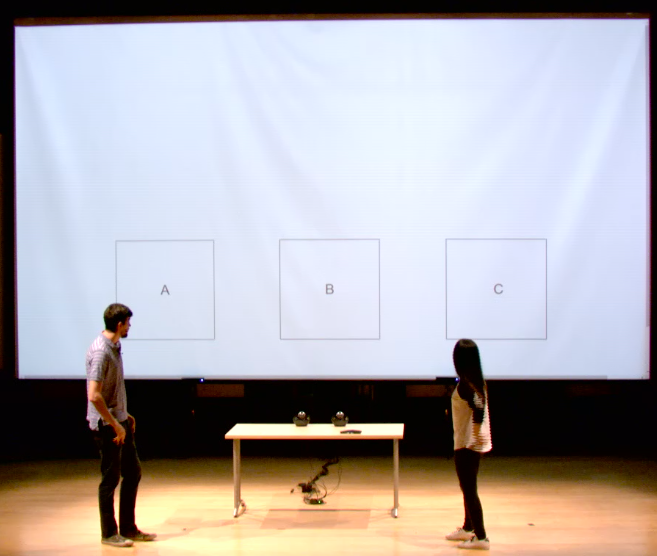
\includegraphics[width=0.7\columnwidth]{chapters/06_planning/figures/blockworld_demo_start.png}
  \caption{Starting state of our system.}
  \label{fig:blockworld_start}
\end{figure}

As a demonstration of our formalization process, we utilize our CAIS to solve the
false-belief task from before, modified to fit our CAIS. To accomplish this,
we instantiate a very elementary blocks world that involves only three blocks
named $\ablock$, $\bblock$, and $\cblock$, which all start on the
table. This is represented in the $\CEC$ as:

\begin{center}
\begin{tabular}{ c c }
    \holds(\on(\ablock, \ctable), 0) & 
    \holds(\clear(\ablock), 0)\\
    \holds(\on(\bblock, \ctable), 0) &     
    \holds(\clear(\bblock), 0)\\
    \holds(\on(\cblock, \ctable), 0) & 
    \holds(\clear(\cblock), 0)
\end{tabular}
\end{center}

In this instantiation, there are then two participants, \humana\ and \humanb\,
and then the block world is shown on the center screen in front of them. This
is shown in Figure~\ref{fig:blockworld_start}. We now provide below a sequence
of events that our agents act upon, providing the formalization of each action
into the \CEC\ as well as the fluent changes at each step of the time. If the
fluent is not removed by a step, then we assume that it carries over from the
previous step as is.

\begin{center}
\begin{tabular}{l | l | l}
    $t$ & Event in Natural Language & Event in \CEC\ \\
    \hline
    1 & \humana\ enters and registers with the CAIS & \happens(\register(\humana), 1) \\
    2 & \humanb\ enters and registers with the CAIS & \happens(\register(\humanb), 2) \\
    3 & \humana\ stacks block \ablock\ onto block \bblock\ & \happens(\stack(\ablock, \bblock), 3) \\
    4 & \humanb\ deregisters and leaves the CAIS & \happens(\deregister(\humanb), 4) \\
    5 & \humana\ unstacks block \ablock\ from block \bblock\ & \happens(\unstack(\ablock, \bblock), 5)
\end{tabular}\label{table:false_belief_actions}
\end{center}

\begin{center}
\begin{tabular}{l | l | l}
    $t$ & Added Fluent & Removed Fluents \\
    \hline
    1 & \holds(\inCAIS(\humana), 1) & \\
    2 & \holds(\inCAIS(\humanb), 2) & \\
    3 & \holds(\on(\ablock, \bblock)), 3) & \makecell[l]{
        \holds(\on(\ablock, \ctable), 2) \\
        \holds(\clear(\bblock), 2) \\
    }\\
    4 & & \holds(\inCAIS(\humanb), 3) \\
    5 & \makecell[l]{
        \holds(\on(\ablock, \ctable), 5) \\
        \holds(\clear(\bblock), 5) \\
    } & \makecell[l]{
        \holds(\on(\ablock, \bblock), 4) \\
    }
\end{tabular}\label{table:false_belief_fluents}
\end{center}

For this test, we utilize our weakest form of vicinity for agents, wherein
all events and fluents that happen within the room are in the vicinity of
any agent in the CAIS, and as such the agent can perceive them. If an agent
is outside the CAIS, then they are considered outside the vicinity of those
events and fluents, and will thus not perceive them. Additionally, for
any agents in the CAIS, they know, per our definition of $\textbf{I}_{1}^{f}$
that then all agents, being in the CAIS not only perceive the fluents for
themselves, but also that they perceive the other agents perceiving those
fluents as well. Additionally, we know from $\textbf{I}_{3}^{f}$ that our
CAIS also perceives all fluent changes, and perceives the agent perceiving
these fluents as well. From instantiations of $R_{1}$ - $R_{4}$ of the \CEC\
inference schemata, we can derive from these perceptions the state of beliefs
of our agents at any given time step to match the fluents that they perceive
at that time step.

\begin{figure}
  \begin{center}
    \begin{minipage}[b]{0.25\textwidth}
      \begin{flushleft}   
        \begin{footnotesize} \underline{\humana's beliefs}\\
          \vspace{4pt}
          \vspace{-4pt}
          \textbf{belief}:
        \end{footnotesize}
      \end{flushleft}    
      \begin{center} \begin{tikzpicture}[auto centering, background rectangle/.style={fill=white}, show background rectangle]
          \node[style=block] (C) {$C$};
          \node[style=empty] (E) [above=of C] {};
          \node[style=block] (B) [left=of C, left=.5cm of C] {$B$};
          \node[style=block] (A) [left=of B, left =.5 cm of B] {$A$};
        \end{tikzpicture}
      \end{center}
    \end{minipage}
   \hspace{50pt}
    \begin{minipage}[b]{0.25\textwidth}
      \begin{flushleft} 
        \begin{footnotesize} \underline{\humanb's  beliefs}\\                          
          \vspace{4pt}
          \vspace{-4pt}
          \textbf{belief}:
        \end{footnotesize}
      \end{flushleft}   \begin{tikzpicture}[auto centering, background rectangle/.style={fill=gray!25}, show background rectangle]
        \node[style=block] (B) {$B$};
        \node[style=emptyA] (E) [above=of C] {};
        \node[style=block] (A) [above=of B] {$A$};
        \node[style=block] (C) [right=of B, right=.5cm of B] {$C$};
        \node[style=empty] (F) [right=of C] {};
      \end{tikzpicture}
    \end{minipage}
  \end{center}
  \caption{Depiction of agents' mental states with the shaded portion indicating that \humanb\ is not in the room.}
  \label{fig:mom-example}
\end{figure}
 
We now move onto solving the false-belief task for our CAIS, and we consider
the world now after the completion of step 5. At this point, we wish to see
where the CAIS believes
the blocks are, as well as where it believes that \humana\ and
\humanb\ think the blocks are, focusing primarily on block A.  We ask
our overseeing AI three questions, translating them into the \CEC:

\begin{center}
\begin{tabular}{l|l}
    Where does the CAIS believe block \ablock\ is? & $\exists x (\believes(CAIS, 5, \holds(\on(\ablock, x), 5)))$ \\
    \makecell[l]{Where does the CAIS believe \\ \hspace{1cm}\humana believe block \ablock\ is?} & $\exists x (\believes(CAIS, 5, \believes(\humana, 5, \holds(\on(\ablock, x), 5))))$ \\
    \makecell[l]{Where does the CAIS believe \\ \hspace{1cm}\humanb believe block \ablock\ is?} & $\exists x (\believes(CAIS, 5, \believes(\humanb, 5, \holds(\on(\ablock, x), 5))))$
\end{tabular}
\end{center}

\noindent
For the first two questions, the CAIS and the \humana\ perceived all fluent
changes within the room, and so the answer should be the same, that block \ablock\ 
is on the table. For the third question, as \humanb\ has left our room, and thus
did not perceive the \unstack\ action, should still believe that the \ablock\
is on \bblock\. This state of affairs is captured in Figure~\ref{fig:mom-example}.
Through \textsf{ShadowProver}, we obtain an answer to the above question
of where each agent believes the block is: 

\begin{center}
\begin{tabular}{l}
     $\believes(CAIS, 5, \holds(\on(\ablock, \ctable), 5))$\\
     $\believes(CAIS, 5, \believes(\humana, 5, \holds(\on(\ablock, \ctable), 5)))$ \\
     $\believes(CAIS, 5, \believes(\humanb, 5, \holds(\on(\ablock, \bblock), 5)))$
\end{tabular}
\end{center}

From this, we have now shown that our CAIS possesses  ``theory of mind'', able to
track beliefs of both itself and contained agents, and moreover answer questions
about it. This provides a valuable baseline of ability to our system as we move
onto planning and plan recognition.

%    3. Single-Step Planning for Intent Resolution

\section{Intent Resolution}

We now move onto utilizing elements of planning, from which we deal with
the problem of intent resolution within our CAIS.
Ideally, any action carried out by our humans within the room would be as explicit
as possible. Indeed, when using something like MUIFOLD, this explicitness is handled for
the user under the hood by the app, tying together what note or block they're interacting
with, and what action they're attempting to accomplish with it. However, through voice,
providing the full explicit action may be difficult or 
impossible~\cite{kephart_embodied_2019}. To demonstrate this
behavior in more exact terms, we provide a motivating example. Imagine that within a CAIS, there
are two agents working with the sticky notes domain. Similar to work shown by
Bolt~\cite{bolt_put-that-there:_1980} a user may point to a note and say "Delete that
note". Alternatively, for reference a note by color on the screen, a user may say "Delete the blue
note". In both cases, while our system provides us with a ``\delete'' intent, we are not
provided an exact note we wish to operate on, and the system has to determine it from
context. We now talk through our algorithm for resolving the intent into something that
is actionable by our system.

\begin{figure}
\centering
  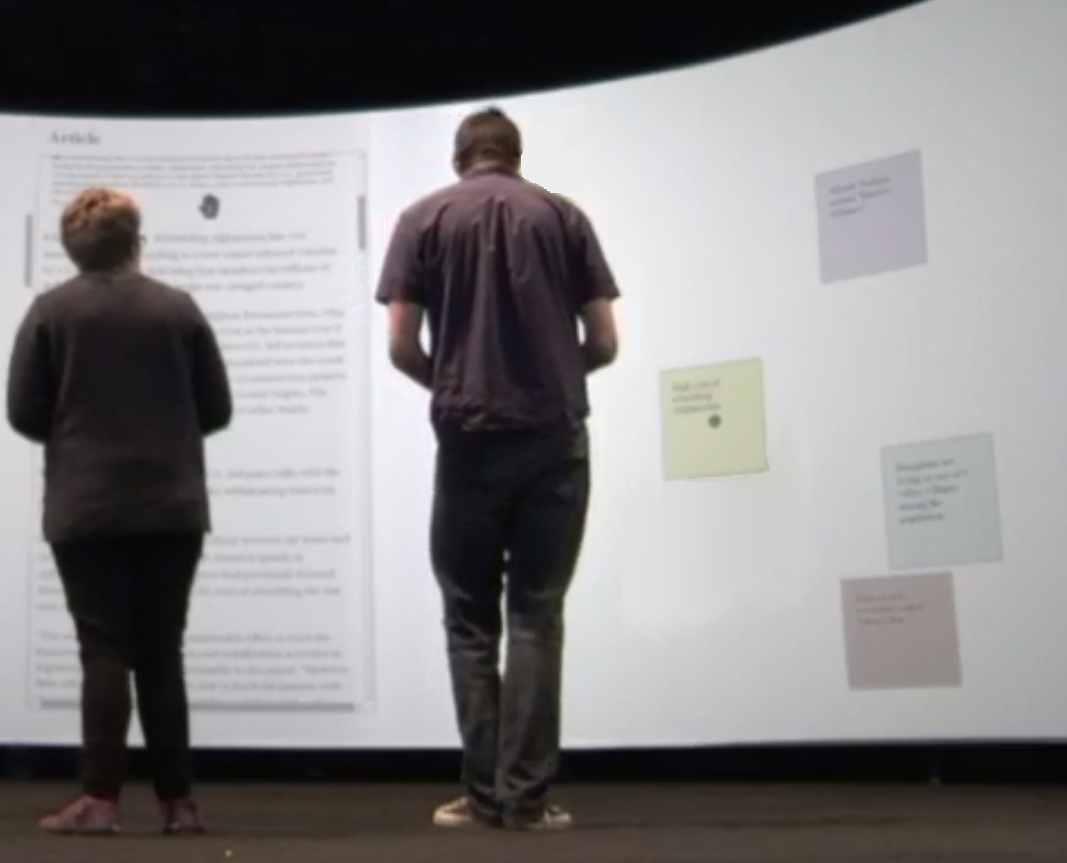
\includegraphics[width=0.7\columnwidth]{chapters/06_planning/figures/intent_sticky_notes.png}
  \caption{Analyst using sticky notes application.}
  \label{fig:intent_sticky_notes}
\end{figure}

We start with grounding our example into a real-world scenario, shown in
Figure~\ref{fig:intent_sticky_notes}. In this scenario, we have two agents once again, \humana\ and
\humanb. There are four notes on the screen, $n1$, $n2$, $n3$, and $n4$ that each have their own color
and location on the screen. Agent \humanb\ is currently pointing at note $n1$ on the screen. We can
axiomatize this set-up as follows:

\begin{center}
\begin{tabular}{ l l l }
    $\holds(\onScreen(n1), 0)$ & 
    $\holds(\position(n1, 50, 50), 0)$ &
    $\holds(\isColor(n1, yellow), 0)$ \\
    $\holds(\onScreen(n2), 0)$ &
    $\holds(\position(n2, 75, 30), 0)$ &
    $\holds(\isColor(n2, purple), 0)$ \\
    $\holds(\onScreen(n3), 0)$ &
    $\holds(\position(n3, 80, 65), 0)$ &
    $\holds(\isColor(n3, blue), 0)$ \\
    $\holds(\onScreen(n4), 0)$ &
    $\holds(\position(n4, 75, 85), 0)$ &
    $\holds(\isColor(n4, red), 0)$ \\
    $\happens(\point(\humanb, n1), 0)$
\end{tabular}
\end{center}

We start first with our example of "Delete that note" as uttered by \humanb. From the conversation-worker,
we receive the \delete\ intent with no further entities. Our orchestrator upon receving the intent then
reaches out to the executor to determine if there are any matching actions to the intent, and receives
the following action, as defined in our STRIPS-style langauge:


\begin{lstlisting}[caption=delete,mathescape=true]
    (define-action delete [(Note ?x)]
        {
            :preconditions [(onScreen ?x)]
            :additions     []
            :deletions     [
                (onScreen ?x)
                $\forall$(y, z) (position ?x y z)
            ]
        }
    )
\end{lstlisting}

From this action, the orchestrator determines that we need a \Note entity to complete the
action, and that we did not receive any such entity from the parsed statement. As such,
the orchestrator then looks to see if it can determine a \Note entity from our context. Here,
it looks through perceived actions of the two agents, scanning in time descending order through
our knowledge base until it finds an action that happened against a note. For our example, it
quickly matches against $\happens(\point(\humanb, n1), 0)$, and given that this action happened
on the same moment as our utterance, then \Note\ $n1$ is deleted. What about had our other agent,
\humana, uttered the statement instead? From our definition of \vicinity\ and its relation to $\perceives$erceiving
as defined in Chapter~\ref{chap:formalizing}, we know that \humana\ has perceived the pointing action
by \humanb. Our orchestrator utilizes that to resolve our intent to the same note in this case.
If both agents were pointing at a note, then the system resolves first to actions committed by that
agent over the ones committed by other agents at the same moment. Finally, the orchestrator
only considers actions that have happened in the recent past (e.g. in the last minute), attempting
to capture the length of attention upon which an agent may give to a particular action or event in
the system. If there is no note that fits our criteria, then the orchestrator issues a request
to the user to clarify which note that they mean.

We now move to our other example of "Delete the yellow note". Similar to above, the orchestrator
gets the same action from the executor and cannot resolve it against any entity in the utterance.
Unlike above however, our utterance contains the \Color\ entity, which is a property of notes and so the
orchestrator then knows that it is additionally looking for a yellow note, or as defined in the
\CEC: $\holds(\isColor(?x, yellow), 0)$. Given this property and the precondition from our action,
our orchestrator generates the query "does there exist a note that is on the screen and is
yellow?" which is formalized as following:

\begin{equation*}
    \exists (\Note\ x) (\holds(\onScreen(x), 0) \land \holds(\isColor(x, yellow), 0))
\end{equation*}

This query is run through \textsf{ShadowProver} as many time as necessary to determine
the candidate set of notes that fit our needs. To accomplish this, for each candidate
returned, we then re-run our query appending a $(x \neq n)$ where $n$ is our discovered
note candidate in the previous step. We keep on appending discovered candidates until the orchestrator
hit a point where \textsf{ShadowProver} can no longer return any matching note. In the case
that the system receives only one note that fits the above query, that note is then removed.
If there are two or more notes, we then utilize a similar algorithm as above, where the
orchestrator scans for actions that relate to any of our candidate notes. If the system
finds any such action within a similar time frame (such as we have in our example), that note
is then used over any other candidate. Similar to above, if there is no way to determine
which note that the user referred to, the system then asks the user to clarify which
note they were referring to.

\begin{figure}
\centering
  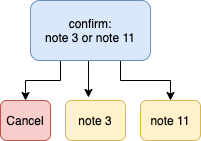
\includegraphics[width=0.3\columnwidth]{chapters/06_planning/figures/intent_resolution_fragment.png}
  \caption{Conditional plan fragment to ask clarification from user.}
  \label{fig:intent_resolution_fragment}
\end{figure}

For cases in which the orchestrator goes back to the user, our system utilizes a similar concept
as employed by Botea et al.~\cite{botea_generating_2019}, where the question to the user
is generated by the orchestrator based on possible candidates and timing, and sets itself up
to expect specific answer types here. For example, let's assume we had two notes that matched
our deletion query. The orchestrator then asks the user for clarification between the two notes
as shown in Figure~\ref{fig:intent_resolution_fragment}, expecting that the response (ignoring
any detected intent) contains one of the notes, or is totally unrelated, thus cancelling the
information request, and continuing as normal. 


%    4. Longer Term Plan Recognition

\section{Plan Recognition for Course Correction}

We finish this chapter with an examination of using plan recognition within our CAIS.
For this, we re-use our scenario from Section~\ref{sect:false_belief}. To re-iterate
the situation, we have two human agents, \humana\ and \humanb, and they are working
in the blocks world domain. Same as before, there are three blocks that are shown
on the screen and they all initially are on the table. This information is
shown below:

\begin{center}
\begin{tabular}{ c c }
    \holds(\on(\ablock, \ctable), 0) & 
    \holds(\clear(\ablock), 0)\\
    \holds(\on(\bblock, \ctable), 0) &     
    \holds(\clear(\bblock), 0)\\
    \holds(\on(\cblock, \ctable), 0) & 
    \holds(\clear(\cblock), 0)
\end{tabular}
\end{center}

This time through, we consider a modified sequence from above, incorporating goals
into the system. On adding a goal to our system, the orchestrator is now set to also
validate all actions taken by agents are in line with the current goals of the system.
Any action that is not valid is then blocked by the orchestrator for proceeding. The
new action sequence is as follows:

\begin{center}
\begin{tabular}{l | l | l}
    $t$ & Event in Natural Language & Event in \CEC\ \\
    \hline
    1 & \humana\ enters and registers with the CAIS & \happens(\register(\humana), 1) \\
    2 & \humanb\ enters and registers with the CAIS & \happens(\register(\humanb), 2) \\
    3 & \humana\ stacks block \ablock\ onto block \bblock\ & \happens(\stack(\ablock, \bblock), 3) \\
    4 & \humanb\ adds goal of block \cblock\ on block \bblock] & \happens(\setGoal(\on(\cblock, \bblock)), 4) \\
    5 & \humanb\ deregisters and leaves the CAIS & \happens(\deregister(\humanb), 5) \\
    6 & \humana\ unstacks block \ablock\ from block \bblock\ & \happens(\unstack(\ablock, \bblock), 6) \\
    7 & \humana\ removes the goal of block \cblock\ on block \bblock\ & \happens(\removeGoal(\on(\cblock, \bblock)), 7) \\
    8 & \humana\ adds the goal of block \ablock\ on block \cblock & \happens(\setGoal(\on(\ablock, \cblock)), 8) \\
    9 & \humana\ stacks block \ablock\ onto block \cblock & \happens(\stack(\ablock, \cblock), 9) \\
    10 & \humanb\ re-enters and registers with CAIS & \happens(\register(\humanb), 10) \\
\end{tabular}\label{table:plan_recognition_actions}
\end{center}

\begin{center}
\begin{tabular}{l | l | l}
    $t$ & Added Fluent & Removed Fluents \\
    \hline
    1 & \holds(\inCAIS(\humana), 1) & \\
    2 & \holds(\inCAIS(\humanb), 2) & \\
    3 & \holds(\on(\ablock, \bblock)), 3) & \makecell[l]{
        \holds(\on(\ablock, \ctable), 2) \\
        \holds(\clear(\bblock), 2) \\
    }\\
    4 & \holds(\goal(\on(\cblock, \bblock)), 4) & \\
    5 & & \holds(\inCAIS(\humanb), 4) \\
    6 & \makecell[l]{
        \holds(\on(\ablock, \ctable), 6) \\
        \holds(\clear(\bblock), 6) \\
    } & \makecell[l]{
        \holds(\on(\ablock, \bblock), 5) \\
    } \\
    7 & & \holds(\goal(\on(\cblock, \bblock)), 6) \\
    8 & \holds(\goal(\on(\ablock, \cblock)), 8) & \\
    9 & \holds(\on(\ablock, \cblock), 9) & \makecell[l]{
        \holds(\on(\ablock, \ctable), 8) \\
        \holds(\clear(\cblock), 8) \\
    } \\
    10 & \holds(\inCAIS(\humanb), 10) & \\
\end{tabular}\label{table:plan_recognition_fluents}
\end{center}

Our diligent \humanb, having returned to the CAIS, sees the state of the world
has moved away from the goal that he set in step 4. He, seeking to achieve that
old goal he still believes is active in the system, attempts to issue the command
"Unstack block A from block C", as he seeks to stack block C onto block B. Our
orchestrator in this case refuses to complete that action as to do so would
move the world away from our goal state of $\on(\ablock, \cblock)$. On refusal
of executing the move, the orchestrator launches into a fallback of plan recognition
over \humanb. The first thing done by the system is to collect the potential goals
that an agent may be following. In this, the system scans through its knowledge base
to find goal addition events that happened within the vicinity of \humanb, giving
us the goals of $\on(\cblock, \bblock)$ and $\on(\ablock, \cblock)$. Next, as per
our definition, the system generates the sequence of actions that would take the
state of the world at the start of step 9 to achieve that goal, giving us an
action sequence. The system finally then takes the action of step 9 and determines
if it within either plan's action sequence. In this case, it finds it as part of
the sequence for the goal of $\on(\cblock, \bblock)$. Taking this information, the
CAIS then scans through its and \humanb's knowledge bases to determine where things
may have gone awry. In this, it determines that \humanb\ did not perceive the goal
state change ate step 6. A summary of this information is then all outputted to the
agents, wherein it shows the agent what plan they were attempting to follow, the plan
that they should have been following, and why they have a difference of information.
This catches the agent up, and their knowledge base is now assumed in regards equal
to that of the room for this sequence.

In addition to utilizing plan recognition above, our CAIS also provides an instantiation
of our property of \textit{Expectation of Usefulness}. This property is
instantiated with the event $e$ being setting a new goal:
$e \equiv \setGoal(\on(\ablock, \cblock)))$:

\begin{footnotesize}
\begin{equation*}
\begin{aligned}
&\perceives\big(\humana, t_8, \happens\big(\setGoal(\on(\ablock,\cblock)), t_{8}\big)\big) \land \perceives\Big(\humana, t_8, \lnot \holds\big(\vicinity(\humanb, setGoal (On(A,C))), t_8\big)\Big) \\
& \hspace{90pt} \rightarrow \believes\Big(\humana, t_{11}, \says\big(\gamma, \humanb, t_{11},
\happens(\setGoal(\on(\ablock,\cblock)), t_8)\big)\Big)
\end{aligned}
\end{equation*}
\end{footnotesize}


% 7. Conclusion
\chapter{CONCLUSION}\label{chap:conclusion}

In this dissertation, we introduced the concept of \textit{cognitive
and immersive systems}, and provided a definition of what constitutes
such a system.  Next, we moved to the architecture, implementation,
and formalization of such a system.  We now look back upon our planned
contributions as enumerated in Section~\ref{sec:contributions}, and
provide some retrospective thoughts pertaining to the work presented
above.  Finally, we share some thoughts regarding future work that
will be developed from the foundational work completed here.

%    1. Thesis Overview
\section{Contributions of the Dissertation, Met}

\begin{enumerate}
    \item \checkmark\ Create a high-level but rigorous and fertile definition for what
        constitutes a CAIS, separating it from a physical robot.

    \begin{itemize}
        \item[] Within this dissertation, we have provided definition for what makes a system
        \textit{cognitive} ($\mathcal{C}$) and what makes it \textit{immersive} ($\mathcal{I}$).
        From these definitions, we can see what an idealized version of a CAIS may look like,
        and indeed, how it a localized physical robot may be able to achieve elements of both
        $\mathcal{C}$ and $\mathcal{I}$, it is not possible to achieve them both fully, or even
        the version presented within this thesis.
    \end{itemize}
  
    \item \checkmark\ Define a framework for how one approaches building a CAIS.
    \begin{itemize}
        \item[] We presented a high-level conceptual framework in
        Section~\ref{sec:cais_architecture} for building out these sorts of systems. Due to the
        high potential number of configurations these systems may be employed into, the framework advocates for
        a modular event-driven system, wherein fusion of sensor data, such as might be needed
        happens downstream from any initial parsing of that sensor. In this purpose, the system
        can handle the loss of a sensor or input mechanism, and that may require the user to
        interact with the system in a different manner, but even there, we can still achieve our
        definition of a CAIS.
    \end{itemize}
    
    \item \checkmark\ Create a real-world implementation of a CAIS, demonstrating at a
  novel level that it:
        \begin{enumerate}
            \item \checkmark\ adapts to a number of potential input mechanisms;
            \item \checkmark\ operates at a true multi-modal and multi-user level; and
            \item \checkmark\ is capable of interacting with and understanding
              third-party content.
        \end{enumerate}
        
    \begin{itemize}
        \item[] Within Chapters~\ref{chap:technology},\ref{chap:reagent},\ref{chap:muifold},
        we created a real world implementation of our CAIS along with several new novel
        technologies to achieve our sub-goals above. From \textit{Reagent}, we demonstrated
        a novel technology that is capable of providing us a functional hook into web-based
        content within the room, understanding what is shown on the page as well as capturing
        and driving user interaction withe content. Additionally, because of its design, Reagent
        can be applied not just to content created specifically for the CAIS, but for most web
        content one might wish to open. Rising from this, we present the \textit{Virtual Mouse API}, wherein
        it allows us to provide all users of our system with their own mouse cursor and ability
        to interact with pages simultaneously with one another. From MUIFOLD, we provide
        a novel framework for building out a UI for cellphones to be used within the CAIS, both
        as a generic pointing device for all users, but also for being able to surface deeper
        interactions with sites that supports it, that would be otherwise impossible on traditional
        pointing devices such as HTC Vive and Kinect cameras. Additionally, due to the modular design
        of all modulars of our system as dictated by our framework, pieces of the work have been
        successfully deployed
        elsewhere~\cite{allen_rensselaer_2019,chabot_collaborative_2020,divekar_humaine_2020}.
    \end{itemize}

    \item \checkmark\ Create a formal definition of a CAIS' implementation and
        its capabilities.
        
    \begin{itemize}
        \item[] In Chapter~\ref{chap:formalizing}, we utilize the \CEC\ drive a formalization of
        our high-level definition. In this way, we provide in exact terms and formulae of the
        cognitive and immersive features discussed in this dissertation. Following this, we also
        provide formalization of the components we utilize in the CAIS, tying together how our
        implementation works and relates to the formalization. Finally, because we have provided
        in exact terms our definitions in this fashion, we were able to derive the property of
        \textit{Expectation of Usefulness}, further separating out a CAIS from a physical robot.
        The formalization, as well as our defined properties and formuale, are to our knowledge
        novel compared to prior work in the space of intelligent or smart rooms.
    \end{itemize}

    \item Utilize the above items to handle tasks of reasoning, planning, and plan recognition
        in and involving a CAIS.
    
    \begin{itemize}
        \item[] Finally, given our implementation and formalization above, we were able to utilize
        these to accomplish tasks in reasoning, planning, and plan recognition, operating at a
        ``theory of mind'' level throughout. Not only that, due to the mechanisms employed, for all
        decisions made by our system, they are fully explainable via a backing proof. Each of these
        demonstrations were deployed and demonstrated in the real-world (albeit against toy domains),
        and that we have shown in highly rigorous terms the power of our cognitive and immersive systems.
    \end{itemize}
\end{enumerate}

%    2. Future Work
\section{Future Work}

We now discuss some promising avenues of future work. We examine two main
thrusts here, within each there are a number of possible extensions and
improvements that may be investigated. The first thrust concerns our
formalization efforts and how we may build upon it. As stated in
Chapter~\ref{chap:formalizing}, we purposely used the \CEC\ to form our
basis, leaving ourselves open to various extensions to it to deal with
more advanced scenarios. Perhaps the biggest extension is to handle the
potentially noisiness of incoming data from sensors and feeding it into
our system. Within this work, we assumed that sensors were providing
perfect information with perfect confidence. In reality, many of the input
mechanisms operate with degrees of confidence on their result. For example,
for each classification that is provided by the conversation-worker, the
Watson Assistant service provides a confidence of its interpretation. For
certain actions, lower allowed confidence levels are fine, such as in the
scenarios presented here, but in more high stakes environments,
the CAIS may need to conduct certain actions only with high confidence and
some with low. To handle this, we look to work by Govindarajulu and
Bringsjord where they incorporate strength factors into a cognitive
calculus~\cite{govindarajulu_strength_2017}. Strength factors can be viewed
as a formalization of part of Chisholm’s rational
belief-fixation~\cite{theory.of.knowledge3.chisholm}. Within the work,
the belief operator is amended such that it has a coefficient, $\sigma$,
such that it ranges from one to five, where beliefs are labelled as (1)
acceptable, (2) some presumption in favor, (3) beyond reasonable doubt,
(4) evident, and (5) certain. An added benefit of this approach is that
the presentation of these strength factors may be easier for understanding
from the layperson versus raw probability values, which people may find
difficult to parse~\cite{kaye_can_1991}.

Another avenue of interest for our formalization efforts is in dealing with 
ethical issues and matters of privacy. When utilizing these collaborative spaces,
as information about specific users grows, a user would have a reasonable
belief that the system will not offer sensitive information to their
colleagues without prior approval. The ``Deontic Cognitive Event
Calculus'' (\DCEC) is an attractive logic to handle these cases, adding in the
deontic operator of obligation on-top of the \CEC. Indeed, Bringsjord et al.
proposes a ``Tenancular AI'' shows the usefulness of the \DCEC\ with regards
to these concerns~\cite{bringsjord_tentacular_2018}. Additionally, the \DCEC\
has been used to model the ethical principals of ``Doctrine of Double
Effect''~\cite{govindarajulu_automating_2017} and ``Doctrine of Triple
Effect''~\cite{peveler_towards_2018}.

The other thrust concerns our technology. First, while we are pleased with
our preliminary results of MUIFOLD and its effectiveness, from it were
identified a number of limitations. The most principle of is in making the
system more robust for how users hold their phones. As identified in
Section~\ref{chap04:limitations} however, we find that users would prefer to
hold their phone at an angle, and then point around that angle. However, our
initial implementation assumed that users were holding their phone flat, which
allowed for a simplification of detecting angle changes only around pitch and
yaw. Implementing roll into the equation would expand usability as we look
to extend our technology into more real-world applications. In that vein,
the evaluation here was preliminary in nature, and a more robust user study
is still required for full evaluation of our technology, especially as it
compares to other mechanisms of relative pointing (e.g. Bluetooth clickers)
and absolute pointers (e.g. Wii remote) both in our laboratory testing, as
well as in real-world usage. Perhaps even more importantly is that the
technology is deployed to real-world usage wherein we may discover additional
issues or strengths only discovered when users engage the technology in a
more natural environment than the Fitts' pointing test.

Finally, the technology and formalization presented here focuses on
co-located environments. This focus was a purposeful one due to the
inherit differences between co-located and distributed that we were
not prepared to address here. The first step towards this would be
working on extending the CAIS implementation we presented here to
a fully distributed set-up, wherein each participant is running their
own transcript-worker, speaker-worker, display-worker, etc., and that
the content to be outputted may be the same, or different per user to
fit their needs, such as the display-workers may have different content
open per user, or the content may be arranged differently. All of this
is to be accounted for within the technology stack, but also must be
incorporated into formalization efforts herein. However, to accomplish this,
our first steps would be on deploying the technology to users for a
given scenario, and perform baseline user studies to understand empirically
real-world usage. From this, we could then better conceptualize and deal
with formalization of the environment, and then bring to bear the fruits
of that formalization effort, such as in intent resolution and plan recognition.



%%%%%%%%%%%%%%%%%%%%%%%%%%%%%%%%%%%%%%%%%%%%%%%%%%%%%%%%%%%%%%%%%%%
%                                                                 %
%                           BIBLIOGRAPHY                          %
%                                                                 %
%%%%%%%%%%%%%%%%%%%%%%%%%%%%%%%%%%%%%%%%%%%%%%%%%%%%%%%%%%%%%%%%%%%

%This method produces a numbered bibliography where the numbers
%correspond to the \cite commands in the text. See the LaTeX manual.
%
\specialhead{REFERENCES}
%\bibliographystyle{abbrv}
\bibliographystyle{IEEEtran}
\bibliography{bib_files/peveler_thesis,bib_files/peveler_misc,bib_files/main72}

% Note that, if you wish, you can use BibTeX to create your bibliography
% from a database. See section 5.6.2 of Memo RPI.110 for information.
%%% Local Variables:
%%% mode: latex
%%% TeX-master: t
%%% End:
 % bibliography
%%%%%%%%%%%%%%%%%%%%%%%%%%%%%%%%%%%%%%%%%%%%%%%%%%%%%%%%%%%%%%%%%%%
%                                                                 %
%                            APPENDICES                           %
%                                                                 %
%%%%%%%%%%%%%%%%%%%%%%%%%%%%%%%%%%%%%%%%%%%%%%%%%%%%%%%%%%%%%%%%%%%
 
\appendix    % This command is used only once!
%\addcontentsline{toc}{chapter}{APPENDICES}             %toc entry  or:
\addtocontents{toc}{\parindent0pt\vskip12pt APPENDICES} %toc entry, no page #

\chapter{THIS IS AN APPENDIX}
This is a sentence to take up space and look like text.
This is a sentence to take up space and look like text.
This is a sentence to take up space and look like text.
This is a sentence to take up space and look like text.

\section{A Section Heading}

This is how equations are numbered in an appendix:
\begin{equation}
x^2 + y^2 = z^2
\end{equation} 
This is a sentence to take up space and look like text.
This is a sentence to take up space and look like text.
This is a sentence to take up space and look like text.
 
This is a sentence to take up space and look like text.
This is a sentence to take up space and look like text.
This is a sentence to take up space and look like text.
This is a sentence to take up space and look like text.
This is a sentence to take up space and look like text. 

\chapter{THIS IS ANOTHER APPENDIX} 
This is a sentence to take up space and look like text.
This is a sentence to take up space and look like text.
This is a sentence to take up space and look like text.
This is a sentence to take up space and look like text.
This is a sentence to take up space and look like text.
This is a sentence to take up space and look like text.
This is a sentence to take up space and look like text.
This is a sentence to take up space and look like text.
 
 % appendix

\end{document}
